\documentclass[12pt]{book}
\usepackage{ctex}
\usepackage{import}
\usepackage{authblk}
\usepackage{amsmath}
\usepackage{graphicx} 
\usepackage{geometry}
\geometry{a4paper,scale=0.8}
\def\celsius{\ensuremath{^\circ\hspace{-0.09em}\mathrm{C}}}
\numberwithin{equation}{section}
\usepackage{tabu}
\usepackage{booktabs}
\usepackage[numbers,sort&compress]{natbib}
\newcommand*{\dif}{\mathop{}\!\mathrm{d}}
\usepackage{caption}
\usepackage[section]{placeins}
\usepackage{float}
\usepackage{placeins}
\DeclareTextFontCommand{\emph}{\bfseries}
\usepackage{verbatim}
\usepackage{amsmath,amssymb}
\usepackage{inputenc}
\usepackage{xeboiboites}
\usepackage{verbatim}
\usepackage{amsmath,amssymb}
\usepackage{braket}
\usepackage{siunitx}
\sisetup{range-phrase = --}
\usepackage{tikz}
\usepackage{pgfplots}
\pgfplotsset{compat=1.16}
\usetikzlibrary{intersections}
\usepackage{pstricks}
\usepackage{makeidx}
%\usepackage{subfigure}
\usepackage[version=4]{mhchem}
\usepackage{multirow}
\usepackage{subfig}
\makeindex
%\usepackage{microtype}

%\usepackage{lipsum}
%opening
\title{材料物理}
\author{Kars}
\date{\today}

\DeclareTextFontCommand{\emph}{\bfseries}


\newboxedtheorem[
small box style={fill=gray!20,draw=black, rounded corners},
big box style={fill=gray!10,draw=orange,thick,rounded corners},
headfont=\bfseries,
thcounter=section]{define*}{Definition}{}

\newboxedtheorem[
small box style={fill=gray!20,draw=black, rounded corners},
big box style={fill=gray!10,draw=orange,thick,rounded corners},
headfont=\bfseries,
thcounter=subsection]{define}{Definition}{definecounter}

\newbreakabletheorem[small box style={draw=orange,fill=blue!20},
big box style={fill=blue!10,draw=orange}]
{theorem}{Theorem}{theoremcounter}
\newbreakabletheorem[small box style={draw=orange,fill=blue!20},
big box style={fill=blue!30,draw=orange}]
{theorem*}{Theorem}{}
\newbreakabletheorem[small box style={fill=white!20,draw=black, 
	rounded corners},
big box style={fill=white!10,draw=orange,thick,rounded corners},
headfont=\bfseries,
broken edges={draw=orange!30!black!20,thick,fill=orange!20!black!5, 
	decoration={random steps, segment length=.5cm,%
		amplitude=1.3mm},decorate},%
other edges={decoration=penciline,decorate,thick}]%
{example}{Example}{examplecounter}    
\newboxedtheorem[small box style={fill=blue!20,draw=black, 
	rounded corners},
big box style={fill=blue!10,draw=orange,thick,rounded corners},
headfont=\bfseries]%
{example*}{Example}{}  

\newboxedtheorem[small box style={fill=blue!10,draw=black, line width=.7pt,
	decoration={penciline},decorate},%
big box style={fill=blue!10,draw=black,thick, 
	decoration={penciline},decorate},
headfont=\bfseries]%
{Proof}{Proof}{}


\newboxedequation[big box style={fill=blue!10,%
	thick,decoration=penciline,decorate}]%
{formula}      



\newbreakabletheorem[small box style={draw=orange,fill=blue!20},
big box style={fill=blue!10,draw=orange},
broken edges={decoration=zigzag}]
{propd}{Proposition}{test}    

\newbreakabletheorem[small box style={draw=orange!30!black!20,%
	fill=orange!10!black!2,decoration=penciline, decorate, thick},
big box style={color=orange!30!black!20,fill=orange!30!black!10,thick},
broken edges={draw=orange!30!black!20,thick,fill=orange!20!black!5, 
	decoration={random steps, segment length=.5cm,%
		amplitude=1.3mm},decorate},%
other edges={decoration=penciline,decorate,thick}]%
{parchment}{Parchment}{test}    

\newparchment[small box style={draw=orange!30!black!20,%
	fill=orange!10!black!2,decoration=penciline, decorate, thick},
big box style={color=orange!30!black!20,fill=orange!30!black!10,thick},
broken edges={draw=orange!30!black!20,thick,fill=orange!20!black!5, 
	decoration={random steps, segment length=.4cm,%
		amplitude=1.7mm},decorate},%
other edges={decoration=penciline,decorate,thick}]%
{parchmentb}{Parchment}{}     

\newspanning[image=dessins/bulb,headfont=\bfseries,%
spanning style={very thick,decoration=penciline,decorate}]%
{method}{Method}{}

\newspanning[image=dessins/poisson,headfont=\itshape,%
spanning style={very thick,decoration=penciline,decorate}]%
{test}{Test}{}
\usepackage{hyperref}
\hypersetup{
	colorlinks,
	citecolor=black,
	filecolor=black,
	linkcolor=black,
	urlcolor=red
}
%\renewcommand\subfigureautorefname{图}
\renewcommand\figureautorefname{图}
\renewcommand\tableautorefname{表}
\renewcommand\equationautorefname{式}
\usepackage{cleveref}
\begin{document}

\maketitle




\clearpage
\frontmatter
\cleardoublepage
\phantomsection
\addcontentsline{toc}{chapter}{前言}
\chapter*{前言}
	本笔记内容来自材料物理课程材料,主要为王学敏老师所教授的部分,而高克玮老师的讲义相对完善,不包含在本笔记内,如有需要,可以尝试完成文件夹中尚未
	完成的三个文档,分别为\href{https://github.com/lkmpoijn/Material_Physics/blob/origin/Chapters/solid_solution.tex}{solid\_solution.tex}、
	\href{https://github.com/lkmpoijn/Material_Physics/blob/origin/Chapters/diffusion.tex}{diffusion.tex}和
	\href{https://github.com/lkmpoijn/Material_Physics/blob/origin/Chapters/phase_transformation.tex}{phase\_transformation.tex}。
	
	参考文献主要是余宗森先生的《金属物理》\cite{余宗森1982高等学校教学用书},Hull的《位错导论》\cite{HULL201143}和R.E. Smallman等人
	的《物理冶金学》\cite{ngan2007physical}。

	这个项目的最初的目的其实仅仅是整理笔记,后来发现一些讲义上不太清晰的内容,又结合其它的资料,然后才形成这个笔记。为了方便他人阅读,
	于是使用\LaTeX 来完成这个项目。由于参考了一些没有找到来源的资料,没有在最后的参考文献标出,因此,如果有侵权问题,
	请及时通知本人。

	文章的图片大部分修改自Hull的《位错导论》\cite{HULL2011137},除非完全不改动,之后就不再用参考文献标出。

	另外关于这个笔记的一点用法,希望各位使用好书后的索引,如果在其中已经加入了超链接,点击页码就可以找到对应的位置,索引按照中文拼音排序。
	
	目前,笔记内容已经上传到\href{https://github.com/lkmpoijn/Material_Physics}{\emph{Github}},欢迎各位同学提出Star和Fork,
	关于\emph{Github}和\LaTeX 的使用方法,请自行在网络上搜索,特别提醒,不要使用百度。

	在本学期后,不会再更新这个项目,除非是重大情况,如果有同学相要继续完成这个项目,可以联系提出issue来催我转移项目。

\cleardoublepage
\phantomsection
\addcontentsline{toc}{chapter}{目录}
\tableofcontents


\mainmatter
\part{晶体缺陷}
	\chapter{点缺陷}
    本部分的内容来自于其他文档,请参考:空位与缺陷.pdf文件。
	\chapter{线缺陷}
    \section{位错概念的引入}
        \subsection{实际晶体的滑移特征}
            在早期对金属材料的范性形变\index{范性形变}的研究中发现:
            \begin{itemize}
                \item[1] 单晶体发生范性形变时表面出现小台阶滑移线;
                \item[2] 晶体滑移总是沿着一定的密排晶面和密排方向,而且只有沿着这些面和方向的切应力达到一个临界值时,滑移才开始进行。
            \end{itemize}
            对与金属单晶来说,这个临界值在\SIrange{1}{10}{\MPa}。在这种情况下,人们引入晶体的理想模型来解决这个问题。

        \subsection{理想晶体的滑移}
            为了解释晶体的变形现象,人们提出了刚性滑移假设\index{刚性滑移假设}。
            假设滑移时滑移面两端的晶体为刚体,原子同步平移,设$T$为加载在晶体上的切应力,在缓慢变形中,该应力与变形相平衡。
            应力大小随滑移面两侧晶体相对位移量变化。

            由于晶体排列具有周期性,点阵对滑移的阻力也是周期性的,变形过程如\autoref{理想晶体变形示意图}所示,
            \begin{figure}[ht]
                \centering
                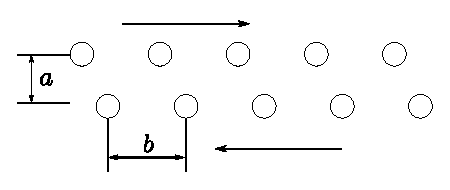
\includegraphics[width=0.7\textwidth]{fig/deformation_of_ideal_crystal.eps}
                \caption{理想晶体变形示意图。}
                \label{理想晶体变形示意图}
            \end{figure}
            
            假定变形所受到的阻力为
            \begin{equation}
                \tau=\tau_m\sin{\left( \frac{2\pi x}{b} \right)}
            \end{equation}
            当发生的变形很小时,可以近似为
            \begin{equation}
                \tau=\tau_m{\left( \frac{2\pi x}{b} \right)},
            \end{equation}
            而且开始变形时,晶体处于弹性阶段,应当满足虎克定律,也就是
            \begin{equation}
                \tau=\mu\gamma=\mu\frac{x}{a},
            \end{equation}
            其中$\mu$为切变模量,$\gamma$为切应变,因此可以得到最大切应力为
            \begin{equation}
                \tau_m=\frac{\mu b}{2\pi a},
            \end{equation}
            由于本课程讨论的晶体绝大多数情况为简单立方晶系,可以认为$a=b$,所以最大切应变为
            \begin{equation}
                \tau_m=\frac{\mu}{2\pi}.
            \end{equation}

            然而理论切变强度$\frac{\mu}{2\pi}$与实际强度相比,实在太大。在使用更为合适的原子间作用力模型后,改变了正弦近似,
            最大切应变数值上降低为原来的$1/60$,但是这仍然比实际值高出了3到4个数量级。

            然而无论如何都提高应力模型的精确程度,最终结果的偏差仍然很大,因此是假设出现了问题。最终人们提出了位错模型,并且在
            实验中观察到了这一现象。
        
    \section{位错的结构}
        晶体中存在三种不同的位错类型,下面将分别描述。
            \subsection{刃型位错}
                考虑一个简单立方晶体,它在$(010)$面上沿$[100]$方向发生滑移,但是这个滑移是不均匀的。
                也就是从晶体的右侧向左传播。在某一时刻,滑移停止在晶体内部。于是在这个$(010)$面左右就可以划分出已滑移区域和未滑移区域,
                该面也就是两个区域的边界。晶体滑移的元过程是在一定的晶体学面上,沿一定的晶体学方向,晶体的上下两部分相对滑移一个或着多个
                点阵常数的距离。

                由此显然可见,已滑移的地区与未滑移的地区是一样的,上述滑移平面上下原子列是恢复对齐的,也就是说,这些地方恢复了理想晶体的长程
                有序性。所以除去\autoref{刃型位错形成示意图}中$\perp$的位置外,晶体的其他部分都是完整的。在这一区域内,晶体的完整周期性显然被
                破坏,所以这就是一个晶体缺陷,称为位错\index{位错}。
                \begin{figure}[ht]
                    \centering
                    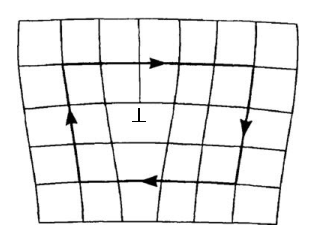
\includegraphics[width=0.45\textwidth]{fig/b_edge_dislocation.eps}
                    \caption{刃型位错形成示意图。}
                    \label{刃型位错形成示意图}
                \end{figure}

                关于位错最为简单的定义就是:位错是近完整晶体中的一个缺陷,是晶体中已滑移区和未滑移区的边界。
                
                这个边界更为严格的说,是分界区域的中心轴线,是平行于$[011]$方向的一条直线,其与滑移矢量$[100]$垂直,那么
                这个位错就称为刃型位错。

                上述中心轴线称为位错线\index{位错线},原理位错线的区域保持理想晶体的完整性;只有极为接近位错线的区域,也就是上述分界区域或
                过渡区域,晶体的点阵结构,或者原子的规则排列被破坏这一区域称为位错核心\index{位错!位错核心}。位错核心的半径与位错线的长度
                相比非常小,所以说,位错是晶体中的线性缺陷。

                对于刃型位错\index{位错!刃型位错},其与滑移矢量垂直,而\autoref{刃型位错形成示意图}中,$\perp$符号代表多余的一个半原子面,
                这个半原子面的边缘就是刃型位错的位错线,形状类似刀刃,因此称为刃位错\index{位错!刃位错}。
                因此刃型位错的形成也可以认为是一个半原子面中断与晶体内部,该边缘也就是一个刃型位错。

                在规定分割面的上下后,半原子面在割面上方的位错称为正刃型位错,反之则为负刃型位错,但是两者并没有本质上的区别。

                刃型位错有以下结构特点
                \begin{itemize}
                    \item[1] 位错周围有弹性畸变或非弹性畸变,上半部分晶体受压力,下部分受张力,中心为最大畸变,畸变局限在2或3个原子间距的管道内,总体为线缺陷;
                    \item[2] 位错线与滑移方向垂直;
                    \item[3] 上下晶体有一个相对位移$\vec{b}$,称为伯格斯矢量或简称柏式矢量\index{柏式矢量}。
                \end{itemize}
            \subsection{螺型位错}
                仍然假定滑移面为$\left( 010 \right)$面,位错线仍然是沿$[001]$方向的直线,但是滑移方向变为$[001]$方向,
                即为与位错线平行的方向,仍然将晶体分为已滑移区、未滑移区以及中间的过渡地带。同样,整个晶体是近完整的,只有在位错核心区,晶体的点阵
                结构才遭到破坏。
                
                也就是说,这也是一个二维缺陷,但是原子排列方式与刃型位错却不相同,不难得出,对与位错线垂直的原子面
                在位错不存在时,是一组彼此平行分立的平面,当此位错存在时,他们则变成一个连续的螺旋面。
                若绕此位错线以左手螺旋正向环行一周,即从一个面上升到相邻的另一个原子面,由于这个形质,这种位错称为螺型位错\index{位错!螺位错}。
                
                \begin{figure}[ht]
                    \centering
                    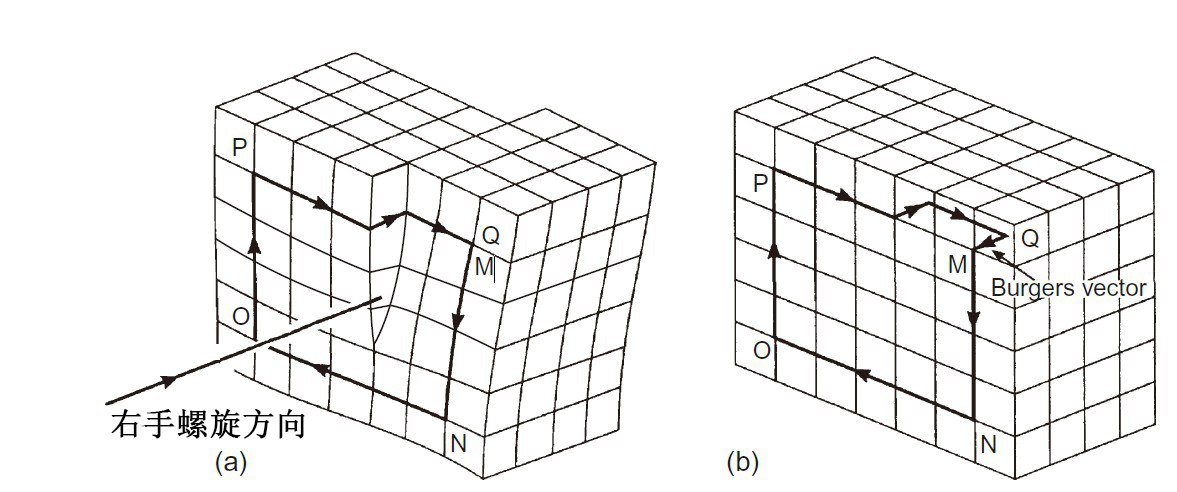
\includegraphics[width=0.7\textwidth]{fig/scheme_of_screw_dislocation.jpg}
                    \caption{右螺型位错示意图,(a)螺型位错的右手螺旋回路,(b)为相同回路在理想晶体中的绕行状况。}
                    \label{螺型位错示意图}
                \end{figure}

                在规定位错线正方向后,若绕位错线以右手螺旋方向绕行一周后,可以上升一个原子面的位错为右螺型位错,如\autoref{螺型位错示意图}
                若绕位错线以左手螺旋方向绕行一周后,可以上升一个原子面的位错为左螺型位错。
                左螺型位错和右螺型位错的滑移矢量方向也是相反的。

                在含有螺型位错的晶体中,原子面排布如\autoref{右螺型位错原子面排布}所示。晶体不再是刃型位错的附加半原子面,而是变成了螺旋式的曲面。
                \begin{figure}[ht]
                    \centering
                    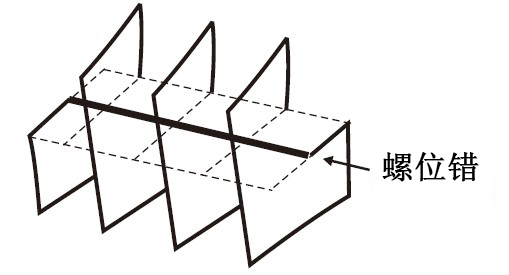
\includegraphics[width=0.5\textwidth]{fig/arrangement_of_atom_in_screw_dislocation.jpg}
                    \caption{右螺型位错原子面排布。}
                    \label{右螺型位错原子面排布}
                \end{figure}
            \subsection{混合型位错}
                然而一根直线位错可能既不与滑移矢量$\vec{b}$垂直,也不平行,而是成一个角度$\theta$,则这个位错既不是纯刃型位错也不是纯螺型位错,
                它可以看作是两个直线位错的叠加,分别为纯刃型和纯螺型的位错,两者的滑移矢量大小为
                \begin{align}
                    \vec{b}_1&=\vec{b}\sin\theta,\\
                    \vec{b}_2&=\vec{b}\cos\theta.
                \end{align}
                这个直线位错称为混合位错\index{位错!混合位错}。组成混合位错的两个分量为刃型分量和螺型分量。

                对上述情况加以推广,假设滑移矢量为$\vec{b}$,已滑移区域为\autoref{混合型位错的滑移示意}中的阴影部分,而位错线为图中红色线,从垂直与滑移面的方向看去,上下两个原子
                面之间的原子排布应该为\autoref{混合型位错的原子排列示意图}所示。
                \begin{figure}[ht]
                    \centering
                    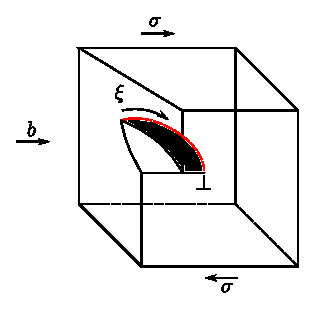
\includegraphics[width=0.5\textwidth]{fig/slip_of_mixed_dislocations.eps}
                    \caption{混合型位错的滑移示意。}
                    \label{混合型位错的滑移示意}
                \end{figure}
                
                \begin{figure}[ht]
                    \centering
                    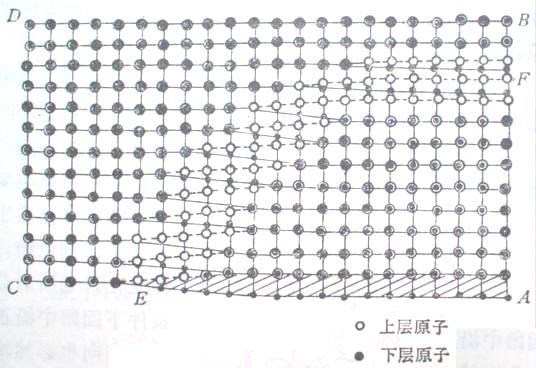
\includegraphics[width=0.5\textwidth]{fig/arrangement_of_atoms_of_mixed_dislocations.jpg}
                    \caption{混合型位错的原子排列示意图。}
                    \label{混合型位错的原子排列示意图}
                \end{figure}
                从\autoref{混合型位错的原子排列示意图}可以看出,这个位错有一段是纯螺型位错,另一端是纯刃型位错,由于位错线是连续的\footnote{这一点需要会证明。}
                从晶体的一个表面延伸到另一个表面,中间弯曲的一端既不是螺型位错也不是刃型位错,而是同时具有螺型和刃型位错的特征。
                这一小段也可以看作是许多方向近连续变化的小直线段所组成,每一小段都是混合型位错,各有一个螺型分量和刃型分量。
            \subsection{小结}
                依照以上定义,位错是晶体中滑移面上两个区域(即已滑移区域和未滑移区域)之间的分界,那么它就应该具有两个重要的性质:
                \begin{itemize}
                    \item[1] 因为晶体的滑移矢量是一个恒定矢量,等于一个或多个最小点阵平移矢量,所以对于一条位错线的各个部分,滑移矢量均相等;
                    \item[2] 无论位错线形状如何,总之位错线绝不可能终止于晶体的内部,位错线只能从晶体的一个表面延伸到另一个表面,或是在晶体中形成一个封闭的环。
                \end{itemize}
        \section{位错的普遍定义与伯格斯矢量}\label{section:位错的普遍定义与伯格斯矢量}
            \subsection{位错的普遍定义}
                在直观的基础上对位错的几何性质有一定的了解以后,我们这里可以对位错作出更为普遍的定义。

                假设晶体沿任意面$S$剖开,将$S$面的两边$S_1$以及$S_2$作一刚性的相对位移$\vec{b}$,$\vec{b}$可以是
                晶体中任意的电子平移矢量\footnote{$\vec{b}$不是点阵矢量的情形将在以后做出讨论。},经过这样的操作以后,
                如果$\vec{b}$与$S$面不平行,有些地方将产生原子位置重叠或者是空隙。去掉重叠的原子,空隙按照晶格排列填补,
                这样$S$面不会有任何改变,但是晶体中出现相对位移和未相对位移区域的分界线,也就是$S$面的周界。在分界线上原子错排的情况就是
                位错线\index{位错线},$\vec{b}$为伯格斯矢量或柏式矢量\index{柏式矢量},其为位错特征的标志,数值大小为$b$,
                称为位错的强度\index{位错!强度}。

                晶体中任意的位错都可以按照上面操作来形成, 但是汽油有一些需要注意的地方:
                \begin{itemize}
                    \item[1] 上述的想象操作不仅是用来说明位错的特征,也模拟了晶体产生位错的实际过程,关于位错生成的过程将以后讨论;
                    \item[2] 对于同一根位错线,可以有不同的$S$面,只要柏式矢量相图,形成的就是相同的位错,因此决定位错特征的是伯格斯矢量,而不是$S$面的具体位置,可以选以位错为边界的任意面作为上述操作的$S$面,比如沿$z$轴的刃型位错,选取$xoz$面和$yoz$面的结果是一致的;
                    \item[3] 实际上,从已经做过相对位移的区域到未作相对位移的区域间的过渡不可能是突变的,否则将产生无法填补的裂缝,因此$S$面两侧的刚性位移在边界是不再适用的,准确到说,位错不是一根线,而是有一定宽度$w$的区域,在这个区域内,$b$从中心的最大值下降到边界的零,只是由于宽度比长度小得多,所以可以近似为一根线。
                \end{itemize}
    
                \subsection{柏式矢量的定义}
                    $\vec{b}$矢量称为柏式矢量,它是位错线特征的标志,位错的强度为$b$,而方向的确定常使用伯格斯回路法和Frank惯例法。
                    \subsubsection{伯格斯回路法}
                        实现选取有位错的实际晶体,从好区中任意原子出发,微扰位错作一个闭合回路,回路每一步都连接相邻的同类原子,并且始终走在晶体的好区,这个回路称为伯格斯回路\index{伯格斯回路}。
                        然后在完整晶体中作一个对应的回路,即在相同方向走相同步数,结果发现这个回路无法闭合。终点到起点的矢量$\vec{b}$为柏式矢量\index{柏式矢量},回路
                        的方向与位错线方向成右手螺旋的方向为正方向。

                        假设晶体中三个基矢量$\vec{a}_0$,$\vec{b}_0$,$\vec{c}_0$,整个晶体的矢量都可以使用这三个矢量表示。
                        在理想晶体中,绕行晶体一周后必然有
                        \begin{equation}
                            \sum_{a}n_a\vec{a}_0+\sum_{c}n_b\vec{b}_0+\sum_{c}n_c\vec{c}_0=0\label{完整晶体的绕行结果},
                        \end{equation}
                        其中$n$为整数。

                        假如晶体不是完善的而是含有点缺陷,\autoref{完整晶体的绕行结果}仍然成立,但是基矢量在不同地方的长度有弹性范围内的差异,
                        这是因为点缺陷附近有弹性畸变,离开点缺陷稍远的地方,弹性畸变相应减少。

                        加入这个封闭回路本身经过的地方都是良好的,但是回路包围的区域中含有一个位错$\vec{b}$,回路的方向与位错的方向构成右手螺旋关系,对这个回路,\autoref{完整晶体的绕行结果}变为
                        \begin{equation}
                            \sum_{a}n_a\vec{a}_0+\sum_{c}n_b\vec{b}_0+\sum_{c}n_c\vec{c}_0=-\vec{b},                            
                        \end{equation}

                    \subsubsection{Frank惯例法}
                        Frank惯例法\index{Frank惯例法}需要线确定位错线的正向,割面及割面法线的正向,按照右手螺旋定则,四个手指顺位错线垂直防御割面上,大拇指指向正半晶体也就是法线方向,规定$\vec{b}$为
                        负半晶体相对与正半晶体的移动方向。

                        在确定$\vec{b}$后,如果位错线与$\vec{b}$平行,则为螺旋位错,方向相同为正,反向为负;如果$\vec{b}$与位错线垂直,
                        则为刃型位错,对于刃型位错的方向,需要使用半原子面右手法,如\autoref{刃型位错的半原子面右手法则}所示。
                        \begin{figure}[ht]
                            \centering
                            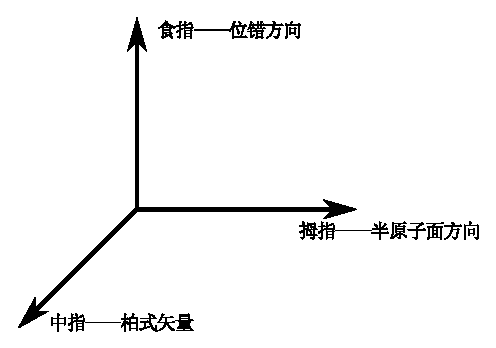
\includegraphics[scale=1]{fig/right_hand_rule_of_edge_dislocation.eps}
                            \caption{刃型位错的半原子面右手法则。}
                            \label{刃型位错的半原子面右手法则}
                        \end{figure}
                \subsection{柏式矢量守恒定律}
                        利用柏式回路的概念即可论证伯格斯矢量的守恒定律:
                        \begin{enumerate}
                            \item[1] 一个位错线不可能中止于晶体内部,它必然构成闭合1的圈或终止于晶体表面,沿一根不分岔的位错线的伯格斯矢量是守恒的,具有相图的大小和方向。
                            \item[2] 如果数根位错线相较于一点,此点称为位错的节点\index{节点},朝向节点的各位错线柏式矢量的总和等于流出各节点位错线伯格斯矢量矢量的总和,如果所有的位错线方向都是从节点出发,则上述关系可以写作各分支柏式矢量的总和为零,即$\sum b=0$;
                            \item[3] 柏式回路有如下特点:
                            \begin{enumerate}
                                \item[1)] 一根位错线只有一个柏式矢量;
                                \item[2)] 位错线不能在晶体内部中断,因而它们只能或者终止在晶体表面,或者形成封闭环,或者与其它位错相联;
                                \item[3)] 当位错与其它位错相联时,指向结点的位错柏氏矢量和与离开节点位错的柏氏矢量和相等,若均指向一个节点,有$\sum b=0$。
                            \end{enumerate} 
                        \end{enumerate}
        
        \section{位错应力场}
            根据\autoref{section:位错的普遍定义与伯格斯矢量},位错是一个线缺陷,其最大畸变分布在以位错线为轴心的管道区域内,管道的直径为2到3个原子间距。
            同时位错的畸变与距离位错线的距离成反比,距离越远的区域,畸变也越小。
            但是由于位错造成的畸变遍布整个晶体,所以伴随这些畸变也造成了晶体各原子之间的位置发生变化,偏离了
            原来的平衡位置,相互之间产生了内应力的作用,应力和应变的乘积即是造成系统能量上升的原因,因此需要定量地分析位错在晶体中所引起的畸变
            和能量。

            为了方便研究,一般把晶体分成两个区域
            \begin{itemize}
                \item[1] 位错中心,由于这个区域畸变严重,必须要考虑晶体结构和原子间相互作用,才能分析应力场和相应的能量;
                \item[2] 远离位错中心的区域,这一部分畸变相对较小,因此可以使用线弹性理论处理。
            \end{itemize}
            
            如\autoref{螺型位错的连续介质模型}所示,沿$z$方向位错线取一个圆柱体,由于中心位置畸变能过大,将其中心挖去,挖掉的区域半径为$r_0$。
            圆柱体沿$z$方向错开一个原子间距$b$,也就是晶体中出现了一个螺位错。假设所研究的点距离中心为$r$,则在绕行一周后,弹性畸变为$b$,平均单位周长变形为
            \begin{equation}
                \varepsilon=\frac{b}{2\pi r}.
            \end{equation}

            \begin{figure}[ht]
                \centering
                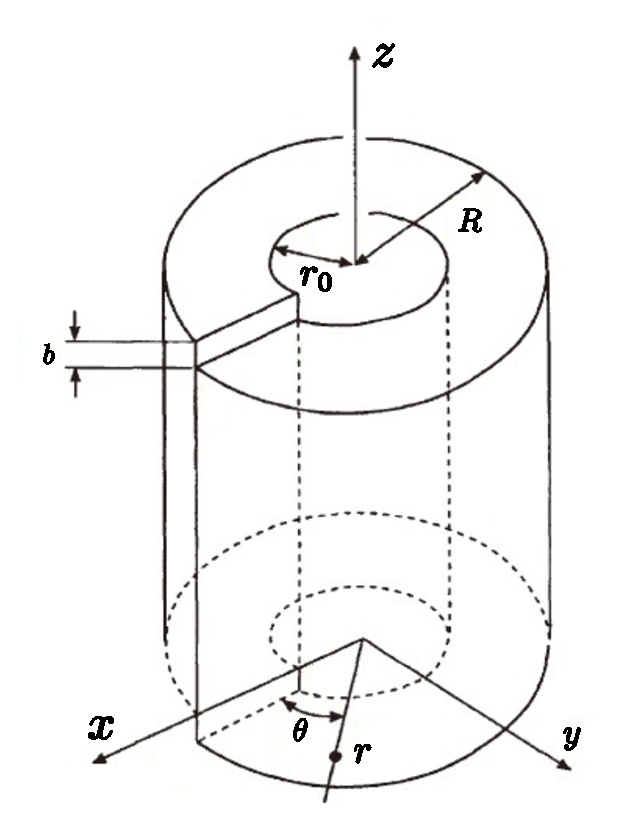
\includegraphics[scale=0.5]{fig/continuous_model_of_screw_dislocation.eps}
                \caption{螺型位错的连续介质模型。}
                \label{螺型位错的连续介质模型}
            \end{figure}

            在柱坐标系中,平均单位周长变形为
            \begin{equation}
                \gamma_{z\theta}=\frac{b}{2\pi r},
            \end{equation}
            由于是弹性变形,代入到胡克定律中,有
            \begin{equation}
                \tau_{z\theta}=\mu\gamma=\frac{\mu b}{2\pi r}, r>r_0.
            \end{equation}
            其中$\mu$为切变模量。

            在直角坐标系中,可以得出
            \begin{align}
                \tau_{xz}&=-\frac{\mu b}{2\pi}\frac{y}{x^2+y^2},\\
                \tau_{yz}&=\frac{\mu b}{2\pi}\frac{x}{x^2+y^2},
            \end{align}
            由此可以看出,
            \begin{itemize}
                \item[1] 在晶体中,只要有位错就有应力场,而不管此晶体是否有外加应力,外加应力与位错产生的应力场无关;
                \item[2] 不同$r$都有应力场,也就是说,位错应力是一个长程应力场,遍布于整个晶体的应力场;
                \item[3] 伴随$r$增大,$\tau$减小,因此距离位错中心越远的地方,应力也就越小;
                \item[4] 根据公式的结果,$r$趋于0,$\tau$为无限大,因此上述公式不再适用于这种情况,这与挖掉位错核心这一方法相符。
            \end{itemize}
            关于位错的应力场的分布则主要是弹性力学的内容,这里不再关注。

            \subsection{刃型位错的应力场}
                假设晶体没有边界,体积无限大,刃位错的位错线沿$z$方向,符号为正,如\autoref{刃型位错的连续介质模型}所示,则
                \begin{figure}[ht]
                    \centering
                    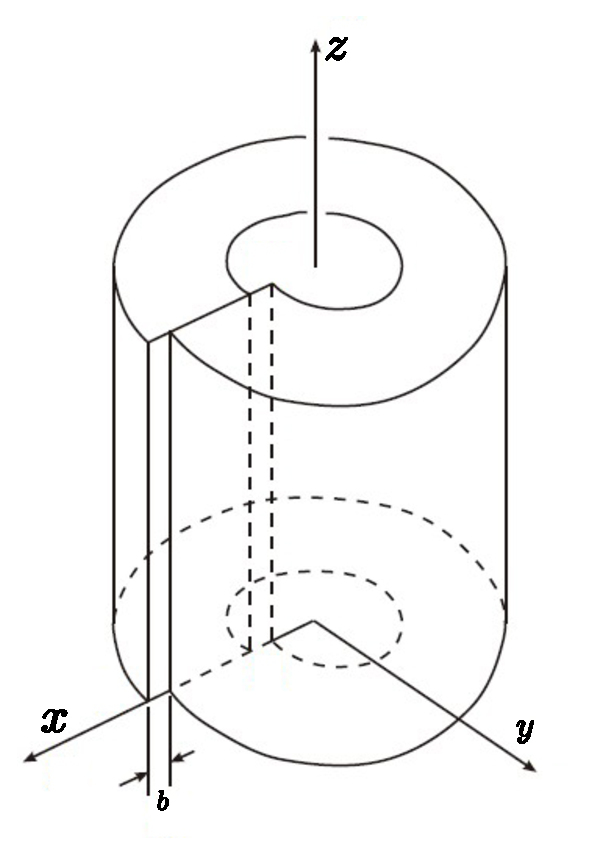
\includegraphics[scale=0.5]{fig/model_of_edge_dislocation.eps}
                    \caption{刃型位错的连续介质模型。}
                    \label{刃型位错的连续介质模型}
                \end{figure}
                应力场的主应力及分量为:
                \begin{align} 
                    \sigma_{x x} &=-\frac{\mu b}{2 \pi(1-v)} \frac{y\left(3 x^{2}+y^{2}\right)}{\left(x^{2}+y^{2}\right)^{2}}\label{刃位错的x主应力}, \\ 
                    \sigma_{y y} &=\frac{\mu b}{2 \pi(1-v)} \frac{y\left(x^{2}+y^{2}\right)}{\left(x^{2}+y^{2}\right)^{2}}\label{刃位错的y主应力}, \\
                    \tau_{x y} &=\frac{\mu b}{2 \pi(1-v)} \frac{x\left(x^{2}-y^{2}\right)}{\left(x^{2}+y^{2}\right)^{2}}\label{刃位错的切应力}, \\
                    \sigma_{z z} &=v\left(\sigma_{x x}+\sigma_{y y}\right)\label{刃位错的z主应力}, \\
                    \tau_{x z} &=\tau_{y z}=0 .
                \end{align}
                其中$v$为泊松比,改用柱坐标系后上述关系变为
                \begin{align}
                    \sigma_{r r}&=\sigma_{\theta \theta}=-\frac{\mu b}{2 \pi(1-v)} \frac{\sin \theta}{r}, \\ 
                    \sigma_{r \theta}&=\frac{\mu b}{2 \pi(1-v)} \frac{\cos \theta}{r}, \\ 
                    \sigma_{z z}&=v\left(\sigma_{r r}+\sigma_{\theta \theta}\right).
                \end{align}
                从刃型位错应力场的表达式可以发现,刃型位错有以下特点
                \begin{enumerate}
                    \item[1] 应力场与$z$方向无关,是平面型的;
                    \item[2] 正应力场关于$yoz$面和$y$轴对称,而且$|\sigma_{xx}|>|\sigma_{yy}|$,
                    \begin{enumerate}
                        \item[a] 当$y>0$也就是上半晶体,$\sigma_{xx}<0$,受压应力,
                        \item[b] 当$y<0$也就是下半晶体,$\sigma_{xx}>0$,受张应力;
                    \end{enumerate} 
                    \item[3] 应力大小与$b$大小有关,而且当$r$增大,应力下降,这与简化分析得到的结果一致;
                    \item[4] $y=0$时,$xoz$面也就是位错的滑移面上有
                            \begin{align}
                                \sigma_{xx}&=\sigma_{yy}=0,\\
                                \tau_{xy}&=\tau_{yx}.
                            \end{align} 
                            也就是切应力在滑移面上有最大值。
                \end{enumerate}
            \subsection{螺型位错的应力场}
                在直角坐标系下,\autoref{螺型位错的连续介质模型}的应力场表达形式为
                \begin{align} 
                    \tau_{x z} &=-\frac{\mu b}{2 \pi} \frac{y}{x^{2}+y^{2}}, \\
                    \tau_{y z} &=\frac{\mu b}{2 \pi} \frac{x}{x^{2}+y^{2}}. 
                \end{align}
                在柱坐标系下,有
                \begin{equation}
                    \tau_{\theta z}=\tau_{z\theta}=\frac{\mu b}{2\pi r},
                \end{equation}
                而其他的应力分量均为0。而螺型位错的应力场的特点为
                \begin{itemize}
                    \item[1]  螺型位错的应力场只有切应力分量,没有正应力分量,所有的正应力分量均等于0。
                    \item[2] 应力大小和$b$有关,并且随着$r$越大、应力越小;
                    \item[3] 应力是轴对称的,与$θ$无关。
                \end{itemize}
            \subsection{混合位错的应力场}
                混合型位错可以采用将柏氏矢量分解的办法进行求解,我们可以发现,位错线平
                行的螺型位错由于没有正应力分量,因此其正应力分量只要采用刃型位错的正应力分
                量即可。
                
                同时刃型位错的切应力分量只有$\tau_{xy}$分量,而螺型位错的切应力分量为$\tau_{xz}$和$\tau_{yz}$,
                因此没有相互重叠的应力分量,可以进行叠加。因此可以总结为如下的特点:
                \begin{itemize}
                    \item[1] 螺型和刃型没有重叠分量;
                    \item[2] 应力场互不影响;
                    \item[3] 因此混合型可以分解为螺型与刃型分量分别计算并叠加。
                \end{itemize}
        \section{位错的应变能}
            前一章已经求出位错的应力场和畸变分布,可以得到,晶体中弹性能量密度为
            \begin{equation}
                \frac{1}{2}\sigma_{ij}\varepsilon-{ij},
            \end{equation}
            由于位错的应力场分为两部分来求解,因此对于位错能量也分为两部分,一部分为位错的核心能量,一部分为周围应力场的能量,也就是应变能,
            利用弹性能量密度,可以得到单位立方体总的应变能
            \begin{equation}
                w=\frac{1}{2}\left(\sigma_{x} \varepsilon_{x}+\sigma_{y} \varepsilon_{y}+\sigma_{z} \varepsilon_{z}+\tau_{x y} \gamma_{x y}+\tau_{y z} \gamma_{y z}+\tau_{z x} \gamma_{z x}\right),
            \end{equation}
            整个弹性题的应变能为
            \begin{equation}
                W=\frac{1}{2}\iiint\sigma\varepsilon\dif v,
            \end{equation}
            但是这一过程非常复杂,求解难度很大。然而采用做功法,利用位错的形成过程,计算这个过程中所做的功,也就是系统能量的增加。

            \subsection{刃型位错的应变能}
                刃型位错形成时可以看作上下半晶体相互推移$\alpha b$,其中$\alpha$在0和1之间,在$\theta=0$处的切应力为
                \begin{equation}
                    \sigma_{\theta r}=\sigma_{r \theta}=\frac{\mu\alpha b}{2\pi(1-v)}\cdot\frac{1}{r},
                \end{equation}
                形成单位长度的位错,做功为
                \begin{equation}
                    \begin{aligned}
                        \dif w&=\frac{\mu\alpha b}{2\pi(1-v)}\cdot\frac{1}{r}\dif r\cdot\dif(\alpha b),\\
                            &=\frac{\alpha\mu b^2}{2\pi(1-v)r}\dif r\dif \alpha,
                    \end{aligned}
                \end{equation}
                对体积元积分,可以得到整个晶体的位错做功
                \begin{equation}
                    \begin{aligned}
                        w_{\text{刃}}&=\int_{r_0}^{r_1}\int_{0}^{1}\frac{\alpha\mu b^2}{2\pi(1-v)r}\dif r\dif \alpha\\
                        &=\frac{1}{2}\alpha^2\lvert_{0}^{1}\cdot\int_{r_0}^{r_1}\frac{\mu b^2}{2\pi(1-v)r}\dif r\\
                        &=\frac{1}{2}\cdot\frac{\mu b^2}{2\pi(1-v)}\ln\left( \frac{r_1}{r_0} \right).
                    \end{aligned}
                \end{equation}
                由于圆柱体内外表面均为自由面条件,因此应该进行修正,修正公式为
                \begin{equation}
                    w_{\text{刃}}\simeq\frac{\mu b^2}{2\pi(1-v)}\left[ \ln\left( \frac{r_1}{r_0} \right) -1\right],
                \end{equation}
                当远离位错核心时,即$r_1\gg r_0$时,这种修正就不重要了。
            \subsection{螺型位错的应变能}
                对于螺型位错的处理与刃型位错的处理接近,晶体之间相互移动$\alpha b$,晶体之间切应力为
                \begin{equation}
                    \sigma_{\theta z}=\frac{\mu\alpha b}{2\pi r},
                \end{equation}
                切应力做功为
                \begin{equation}
                    \begin{aligned}
                        w_{\text{螺}}&=\int_{r_0}^{r_1}\int_{0}^{1}\sigma_{\theta z}b\dif r\dif \alpha\\
                        &=\int_{r_0}^{r_1}\int_{0}^{1}\frac{\mu b^2}{2\pi r}\dif r\alpha\dif \alpha\\
                        &=\frac{\mu b^2}{2\pi r}\ln\left( \frac{r_1}{r_0} \right).
                    \end{aligned}
                \end{equation}
                修正后为
                \begin{equation}
                    w_{\text{螺}} =\frac{\mu b^2}{2\pi r}\left[ \ln\left( \frac{r_1}{r_0} \right)-1 \right].                    
                \end{equation}
            \subsection{混合型位错的应变能}
                由于混合型位错的应力场可以将混合型位错分解为螺型分量和刃型分量再求出各
                自的应力场分量后进行叠加,从而应变能也可以先分解,再进行叠加即可。

                假设柏式矢量$\vec{b}$与位错线夹角等于$\psi$,则刃型位错和螺型位错的分量为
                \begin{align}
                    \text{刃型位错:}&b_\perp=\vec{b}\sin\psi,\\
                    \text{螺型位错:}&b_\parallel=\vec{b}\cos\psi.\\                
                \end{align}
                由于同向刃型位错与螺型位错无相互作用,两者可以叠加
                \begin{equation}
                    w_{\text{混}}=\frac{\mu b^{2} \sin ^{2} \psi}{4 \pi(1-v)} \ln \left(\frac{r_{1}}{r_{0}}\right)+\frac{\mu b^{2} \cos ^{2} \psi}{4 \pi} \ln \left(\frac{r_{1}}{r_{0}}\right),
                \end{equation}
                或者写为:
                \begin{align}
                    w_{\text{混}}=\frac{\mu b^{2}}{4 \pi K} \ln \left(\frac{r_{1}}{r_{0}}\right),\\
                    \frac{1}{K}=\cos^2\psi+\frac{\sin^2\psi}{1-v}.
                \end{align}
                从应变能的表达式可以看出:
                \begin{itemize}
                    \item[1] 应变能和$b^2$成正比,刃型比螺型差一个因子,由于一般金属材料泊松比在0.3左右,也就是说,相同位错强度的刃型位错比螺型位错的应变能大50\%左右;
                    \item[2] 接近位错核心时,公式不再适用,通常情况下,位错核心能是应变能的十分之一;
                    \item[3] 对于一般金属,位错应力场范围受到亚晶界的限制,所以$r_1\simeq\SI{1e-4}{\cm}$,而$r_0\simeq\SI{1e-8}{\cm}$,因此在原理位错核心区有
                    \begin{equation}
                        w_{\text{混}}\simeq\mu b^2=\alpha\mu b^2,
                    \end{equation} 
                    其中$\alpha$在\numrange{0.5}{1}之间,因为位错的应变能相当大,在位错的自由能的表达式
                    中,应变能是主要的项,所以位错不是热平衡自由能最低的产物,这一点和空位不
                    同。
                \end{itemize}
        \section{位错的线张力}
            已知位错的能量与它的长度成正比,若要增加位错的长度,必须做功,因此,围殴错总是有收缩其长度的趋势,
            这表明在能量的意义上将,位错线表现有线张力。可以定义位错线张力等于位错线伸长一个单位长度所做的功,
            用$T$表示。一个直位错的张力等于
            \begin{equation}
                \begin{aligned}
                    T&=\frac{\partial W}{\partial l}\\
                    &=\frac{\mu b^{2} \sin ^{2} \psi}{4 \pi(1-v)} \ln \left(\frac{r_{1}}{r_{0}}\right)\left(1-v \cos ^{2} \psi\right)\\
                    &\simeq \frac{1}{2}\mu b^2.
                \end{aligned}
            \end{equation}
            但是,位错的张力多少和位错的形状有关,上式所指的是直的位错。对于一般波
            浪形的位错,其张力基本上也可以用式,证明从略。故在以后的应用中均用此公式表
            示位错的线张力。
        \section{位错核心}
            在讨论应力场和应变能的时候,都提到由于位错核心\index{位错核心}区域的畸变太大,不能用线弹性理论来求解,必须引入点阵的周期性,并结合连续
            介质的结果处理一系列问题:位错核中心的宽度,位错在点阵中运动的阻力和位错中心能量的问题。

            但是点阵模型不是彻底的,仍然要采纳某些观点和结果,所以只使用一个半点阵模型。

            这一节的点阵模型最早由Peiels提出,后来Nabarro对这一模型进行了修正,因此称为
            Peiels-Nabarro模型,简称派-纳模型\index{位错核心!派-纳模型}。
            \subsection{点阵模型}
                以简单立方晶体的刃型位错为例,位错可以视为由两个完成的半晶体拼接而成。
                \begin{figure}[ht]
                    \centering
                    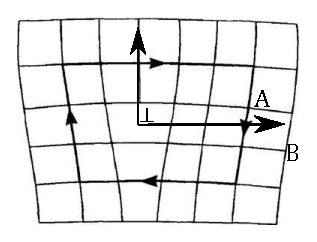
\includegraphics[width=0.5\textwidth]{fig/coordinate_in_edge_dislocation.eps}
                    \caption{刃型位错模型。}
                    \label{刃型位错模型}
                \end{figure}

                设原子间距为$\Phi$,在拼合之前,横轴方向的原子间距为
                \begin{equation}
                    \begin{aligned}
                        \Phi&=\frac{1}{2}b,x>0,\\
                        \Phi&=-\frac{1}{2}b,x<0.
                    \end{aligned}
                \end{equation}
                在拼合后,上下两层分别受到压力和张力,使得原子尽量对齐,在这一过程中,假设上半晶体中位错核心层的
                原子发生了位移$u(x)$,则有
                \begin{equation}
                    \begin{aligned}
                        x>0,u(x)<0,\\
                        x>0,u(x)>0.
                    \end{aligned}
                \end{equation}
                而原子间距则变为
                \begin{align}
                    \Phi(x)=2u(x)+\frac{b}{2},x>0\label{位错正向的原子的位移},\\
                    \Phi(x)=2u(x)-\frac{b}{2},x<0.
                \end{align}
                距离位错核心无穷远时,位错的影响忽略不计,也就是$\Phi(\pm\infty)=0$,所以有
                \begin{equation}
                    u(\infty)=-u(-\infty)=-\frac{b}{4}.
                \end{equation}
                \begin{figure}[ht]
    \centering
    \begin{tikzpicture}
        \begin{axis}[
            xlabel={$x$},
            ylabel={$u(x)$},
            xtick=\empty,
            ytick=\empty,
            axis y line =center,
            axis x line =center,
        ]
            \addplot[blue,thin,domain=0:5,samples=100] {exp(-x)-1};
            \addplot[blue,thin,domain=-5:0,samples=100] {-exp(x)+1};
            \addplot [black,thin,dashed,domain=-5:5] {1.08}
                node [pos=0.75,anchor=north] {$\frac{b}{4}$};
            \addplot [black,thin,dashed,domain=-5:5] {-1.08}
                node [pos=0.25,anchor=south] {$-\frac{b}{4}$};
        \end{axis}
    \end{tikzpicture}
    \caption{原子平衡位置的偏离与位错核心距离的关系。}
    \label{原子平衡位置的偏离与位错核心距离的关系}
\end{figure}

                为求出相应的位移,以及各个原子之间的畸变,Peierls假定上下两层之间的作用力为周期性,
                位错管道外为连续介质,这样,两层原子之间的吸引产生了切应力$\sigma_{yx}$,
                \begin{equation}
                    \sigma_{yx}=\frac{\mu}{2\pi}\left( \frac{b}{a} \right)\sin\left( \frac{2\pi\Phi}{b} \right),x>0,
                \end{equation}
                代入\autoref{位错正向的原子的位移},可得
                \begin{equation}
                    \sigma_{yx}=-\frac{\mu}{2\pi}\left( \frac{b}{a} \right)\sin\left( \frac{4\pi u(x)}{b} \right),x>0,                    
                \end{equation}
                当$\Phi$很小时,没有发生塑性形变,因此可以使用虎克定律
                \begin{equation}
                    \sigma_{yx}=\frac{\mu}{2\pi}\left( \frac{b}{a} \right)\sin\left( \frac{2\pi\Phi}{b} \right)=\mu\left( \frac{\Phi}{a} \right)\label{刃位错核心引起的切应力公式1}.
                \end{equation}

                同时为了求出上半部材料的切应力,EShelby提出柏式矢量为$\vec{b}$的位错可以
                看作是无穷小位错分布在滑移面上,柏式矢量之和等于$\vec{b}$,且分布不均匀。
                设分布在$x^{\prime}\to x^{\prime}+\dif x^{\prime}$之间的柏式矢量为$f(x^{\prime})$
                因此总的柏式矢量为
                \begin{equation}
                    \int_{-\infty}^{^\infty}f(x^{\prime})\dif x^{\prime}=\vec{b},
                \end{equation}
                分布在$x^{\prime}\to x^{\prime}+\dif x^{\prime}$之间的切应力为$\frac{\mu f(x^\prime)}{2\pi(1-v)}\cdot\frac{(x-x^{\prime})^3}{(x-x^\prime)^4}\dif x^{\prime}=\frac{\mu f(x^\prime)}{2\pi(1-v)}\frac{\dif x^{\prime}}{x-x^{\prime}}$
                在两层原子之间的切应力为
                \begin{equation}
                    \sigma_{y x}=\frac{\mu}{2 \pi(1-v)} \int_{-\infty}^{\infty} \frac{f\left(x^{\prime}\right) d x^{\prime}}{x-x^{\prime}}, x^{\prime}>0\label{利用不均匀位错导出的核心切应力1},
                \end{equation}
                当$x=x^\prime$时,有
                \begin{equation}
                    \dif u(x^\prime)=f(x^\prime)\dif x^\prime,
                \end{equation}
                \autoref{利用不均匀位错导出的核心切应力1}可以写作
                \begin{equation}
                    \sigma_{y x}=-\frac{\mu}{\pi(1-v)} \int_{-\infty}^{\infty} \frac{\frac{d u\left(x^{\prime}\right)}{d x^{\prime}} d x^{\prime}}{x-x^{\prime}}, x>0\label{刃位错核心引起的切应力公式2},
                \end{equation}
                
                联立\autoref{刃位错核心引起的切应力公式1}和\autoref{刃位错核心引起的切应力公式2},解得
                \begin{equation}
                    u(x)=-\frac{b}{2\pi}\arctan\left( \frac{x}{\xi} \right),\xi=\frac{a}{2(1-v)},
                \end{equation}
                当$x=0$,$u(x)=0$,而$\Phi=\frac{b}{2}$,在无穷远处,$u(x)=\frac{b}{4}$,此时$\Phi=0$,
                这与之前的结果一致。位错管道附近的错排值分布如\autoref{错排值沿滑移面的分布}所示。

                \begin{figure}[ht]
    \centering
    \begin{tikzpicture}
        \begin{axis}[
            xlabel={$x$},
            ylabel={$\left\vert\Phi\right\vert$},
            xtick=\empty,
            ytick=\empty,
            axis y line =center,
            axis x line =bottom,
            ymax=1.5,
        ]
            \addplot[blue,thin,domain=0:5,samples=100] {1-2*rad(atan(1.4*x))/3.1415}
                node[pos=0,black,anchor=east] {$\frac{b}{2}$};
            \addplot[blue,thin,domain=-5:0,samples=100] {1-2*rad(atan(-1.4*x))/3.1415};
            \addplot[dashed,black,domain=-0.75:0.75] {0.5}
                node[pos=0.35, anchor=north] {$\omega$};
        \end{axis}
    \end{tikzpicture}
    \caption{错排值沿滑移面的分布。}
    \label{错排值沿滑移面的分布}
\end{figure}
                
                从图中把畸变的半高宽定义为位错的宽度,因此位错的宽度为
                \begin{equation}
                    \omega=2\xi=\frac{a}{1-v},
                \end{equation}
                对于泊松比为0.3的材料,位错的宽度约为$1.5a$。
            \subsection{位错引起的晶体错排能}
                前面已经提到,用连续介质中位错的模型可以求出弹性畸变区的能量,但不能求
                出位错中心的能量。现在我们可以根据上述点阵模型对这部分能量做一个估计。位错
                总的应变能包括两部分,即$\omega_0$就是以前求过的弹性区的能量,$\omega_{AB}$
                是由于位错中心附近滑移面上下两层原子没能对齐的能量——错排能。

                由于错排实际只在位错附近,所以这部分能量属于位错中心区的能量。
                先求解弹性区的应变能$W_0$,根据点阵模型得到的应力表达式,代入后可以求得
                \begin{equation}
                    \begin{aligned}
                        W_{0}&=\frac{1}{2} \int_{\xi}^{r_{1}} \sigma_{y_{x}} b \dif x\\
                        &=-\frac{\mu b^{2}}{4 \pi a} \int_{\xi}^{r_{1}} \sin \frac{4 \pi u(x)}{b} \dif x\\
                        &=\frac{\mu b^{2}}{4 \pi a} \int_{\xi}^{r_{1}} \sin \left[2 \arctan\left(\frac{x}{\xi}\right)\right] \dif x
                    \end{aligned}
                \end{equation}
                由于位错是长程应力场,$r_1\gg\xi$,因此有
                \begin{equation}
                    W_0\simeq\frac{\mu b^2}{4\pi(1-v)}\ln\frac{r_1}{\xi}.
                \end{equation}
                然后求解错排能,在计算应变能时,假定位错宽度以外滑移面两侧的晶体发生
                刚性滑移,然而这在位错核心区不再适用,在上节计算错排能的时候,为了强调点阵模型.所以用代数的加
                法,这是为了要显示出位错偏离出对称位置以后能量的变化。做为近似,假如如不需
                要求点阵阻力,我们仍然可用积分代替相加两层的对应原子的错排能已知等于
                \begin{equation}
                    \frac{\mu b^{3}}{4 \pi^{2} a}\left(1+\cos \frac{4 \pi u(x)}{b}\right)=\frac{\mu b^{3}}{2 \pi^{2} a} \cos ^{2}\left(\frac{2 \pi u(x)}{b}\right)=\frac{\mu b^{3}}{2 \pi^{2} a} \cos ^{2}\left(\arctan \frac{x}{\xi}\right),
                \end{equation}
                错排能的表达式为
                \begin{equation}
                    W_{AB}\simeq\frac{\mu b^2}{2\pi(1-v)},
                \end{equation}
                这一数值与应变能相比,差了一个系数$\ln\left( \frac{r}{\xi} \right)$,如果$r=\SI{1e-4}{\cm}$,
                $\xi$为\SI{1e-8}{\cm},则可以计算处错排能大约为应变能的0.1。
            \subsection{点阵阻力}\label{subsection:点阵阻力}
                平衡的条件下,位错处于平衡位置,如果位错中心发生了$\alpha b$的滑移,系统的能量也会发生变化,
                这一变化的梯度造就了位错移动的阻力。这样,计算的关键在于求出位于位错偏离出对称位置时,由于滑
                移面上下两层原子没有对齐而引起的能量。假设\autoref{刃型位错模型}中AB两层原子对齐时作用能为零。
                考虑A层任意一行与纸面垂直的原子,这一行原子与位错平行,并且为单位长度,它所受的力$F$若按照
                连续介质的观点是分布在面积$b$上面的,
                这一行原子所受的力为
                \begin{equation}
                    F=\sigma_{xy}b\label{位错核心受到的力与柏式矢量关系},
                \end{equation}
                因此可以说这一行原子和B层对应原子因为没有对齐而具有能量,也就是错排能,其等于
                \begin{equation}
                    \frac{1}{2}\int_{0}^{\Phi}\sigma_{yx}b\dif \Phi,
                \end{equation}
                其中的系数$1/2$是因为原子之间的势能分配在A 和B 两部分的值将取自\footnote{这里有缺漏,希望有人补完。}
                。因此在A层与$z$轴平行的单位长度的一行原子具有的错排能为
                \begin{equation}
                    \begin{aligned}
                        V_{u(x)}&=-\frac{1}{2}\left(\frac{\mu b^{2}}{2 \pi a}\right) \int \sin \frac{4 \pi u(x)}{b} d(2 u) \\ 
                            &=-\frac{\mu b^{3}}{8 \pi^{2} a} \int \sin \frac{4 \pi u}{b} d\left(\frac{4 \pi u}{b}\right) \\ 
                            &=\frac{\mu b^{3}}{8 \pi^{2} a}\left(\cos \frac{4 \pi u}{b}\right)+C.
                    \end{aligned}
                \end{equation}
                $C$为积分常数,已知当$u=\pm\frac{b}{4}$时,错排能为零,可以求出$C$:
                \begin{equation}
                    C=-\frac{\mu b^{3}}{8 \pi^{2} a} \cos \left(\frac{4 \pi}{b} \cdot \frac{b}{4}\right)=\frac{\mu b^{3}}{8 \pi^{2} a},
                \end{equation}
                回代得到
                \begin{equation}
                    V_{u(x)}=\frac{\mu b^{3}}{8 \pi^{2} a}\left[1+\cos \frac{4 \pi u(x)}{b}\right].
                \end{equation}
                若位错正好位于对称位置,则A和B两层全部原则为位置可以写作
                \begin{equation}
                    x=\frac{1}{2}nb,n=0,\pm1,\pm2\cdots
                \end{equation}
                当位错中心发生$\alpha b$的位移后,原子位置近似可以表示为
                \begin{equation}
                    x=\left( \alpha+\frac{1}{2}n \right)b,
                \end{equation}
                这样错排能变为
                \begin{equation}
                    \begin{aligned}
                        V&=\frac{\mu b^{3}}{8 \pi^{2} a} \sum_{-\infty}^{+\infty}\left[1+\cos \frac{4 \pi}{b}\left\{-\frac{b}{2 \pi} \arctan \frac{\left(a+\frac{1}{2} n\right)}{\xi} b\right\}\right] \\
                        &=\frac{\mu b^{3}}{8 \pi^{2} a} \sum_{-\infty}^{+\infty}\left[1+\cos 2\left\{\arctan \frac{\left(a+\frac{1}{2} n\right)}{\zeta} b\right\}\right].
                    \end{aligned}
                \end{equation}
                单个原子的势能可以写作
                \begin{equation}
                    V_{\alpha}=\frac{\mu b^{2} \xi}{\pi a} \sum_{s=1}^{\infty} e^{-4 x \xi_{s} / b} \cos 4 \pi a s,
                \end{equation}
                将$\xi=\frac{a}{2(1-v)}$代入得到
                \begin{equation}
                    V_{a}=\frac{\mu b^{2}}{2 \pi(1-v)} e^{-4 \pi \xi / b} \cos 4 \pi \alpha,
                \end{equation}
                位错运动受到的力为
                \begin{equation}
                    F=\frac{-\partial V_\alpha}{\partial(\alpha b)}=\frac{-1}{b}\frac{\partial V_a}{\partial\alpha}=\frac{2\mu b}{1-v}e^{-\frac{4\pi\xi}{b}}\sin{4\pi\alpha},
                \end{equation}
                其最大值为$F_{\mathrm{max}}=\frac{2 \mu b}{1-\nu} e^{-4 \pi \xi / b}$。
                根据\autoref{位错核心受到的力与柏式矢量关系},刃位错运动受到的切应力为
                \begin{equation}
                    \sigma_{e}=\frac{2 \mu}{1-v} e^{\frac{-i \pi \xi} { b}}=\frac{2 \mu}{1-v} e^{ -\frac{2 \pi a}{b(1-v)}},
                \end{equation}
                称为点阵阻力\index{点阵阻力},也称作派-纳力。
            \subsection{小结}
                \begin{itemize}
                    \item 位错的核心能约为$\frac{1}{10}\mu b^2$,也就是应变能的$1/10$;
                    \item 位错的宽度认为是$\omega=1.5a$,$a$为晶格常数;
                    \item 点阵阻力$\tau$取决于点阵阻力$a$和柏式矢量$b$,当点阵常数增大时,阻力减小。
                \end{itemize}
        \section{位错的受力与运动}
            \subsection{位错的运动方式}
                晶体在受到适当的应力时,位错可以发生运动,其实在构造位错的示意中就可以
                发现,如果应力继续施加,实际产生的效果就是位错的滑移。位错的运动方式分为
                滑移和攀移。

                滑移指位错滑移在滑移面上的运动,滑移面是位错线和柏式矢量确定的平面,法线方向为$\vec{l}\times \vec{b}$。
                而攀移是指位错垂直于滑移面上的运动。对于这两种运动,下面将分为刃型位错和螺型位错讨论。

                对于刃型位错,滑移过程如\autoref{刃型位错滑移时周围原子的动作}所示,设晶体中已有一个刃型位错,在外加
                切应力作用下,这个位错发生运动,可使晶体上下发生相对移动的区域逐渐扩大。当位错移出晶体的时候就是获赠个晶体
                上下两部分已经完成了相对移动一个原子间距。表示随着刃型位错在晶体中扫过的各个阶段所造成的变形。是位错在晶体
                尚未移出晶外,位错扫过整个滑移面时,就会造成永久切变。
                \begin{figure}[ht]
                    \centering
                    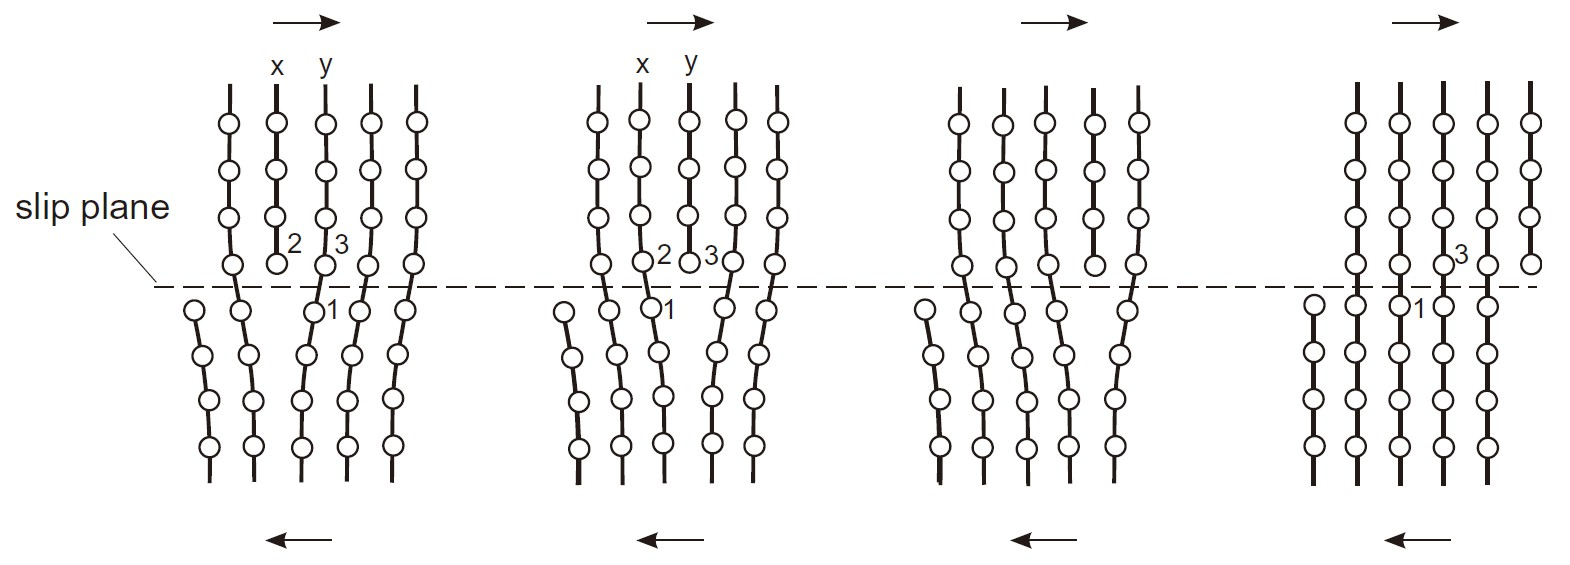
\includegraphics[width=0.7\textwidth]{fig/movement_of_edge_dislocation.jpg}
                    \caption{刃型位错滑移时周围原子的动作。}
                    \label{刃型位错滑移时周围原子的动作}
                \end{figure}
                
                从\autoref{刃型位错滑移时周围原子的动作}中可以看出,位错周围的原子只要发生微小的位移就可以造成
                位错的滑移,且位错的滑移不需要物质的长程迁移,所以位错运动传递的是一个组态,也就是原子错排的组态,
                而且滑移过程中位错的运动方向与位错线方向垂直,与位错的正负号无关,刃型位错在切应力方向运动,晶体
                上出现的台阶与位错线是平行的。

                研究发现,晶体中密排面上的位错易于滑动,这与密排面的晶面间距大,点阵阻力小有关。对于螺型位错,其
                滑移过程如\autoref{螺型位错滑移示意图}所示。螺位错周围的原子如\autoref{螺位错滑移时位错周围原子的动作}
                所示,同样只要位错周围的原子发生微调,位错就会发生滑移,而且位错的运动方向与位错线垂直,但是位错
                线移动方向与切应力垂直,这一点与刃位错不同。晶体上出现的台阶与位错线是垂直的。
                \begin{figure}[ht]
                    \centering
                    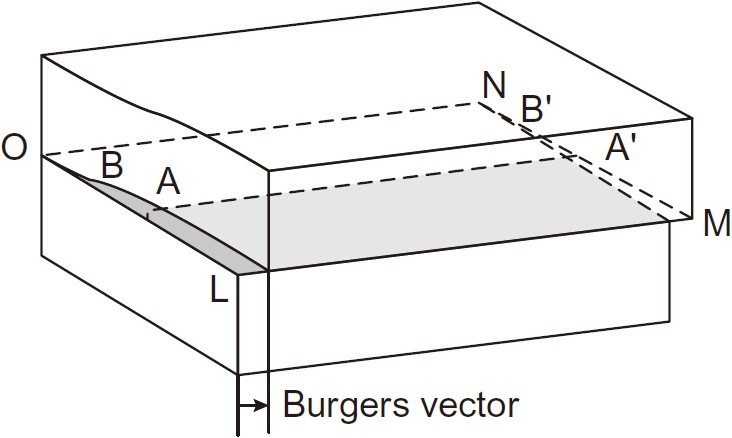
\includegraphics[width=0.5\textwidth]{fig/movement_of_screw_dislocation.jpg}
                    \caption{螺型位错从$AA'$运动到$BB'$示意图。}
                    \label{螺型位错滑移示意图}
                \end{figure}
                \begin{figure}[ht]
                    \centering
                    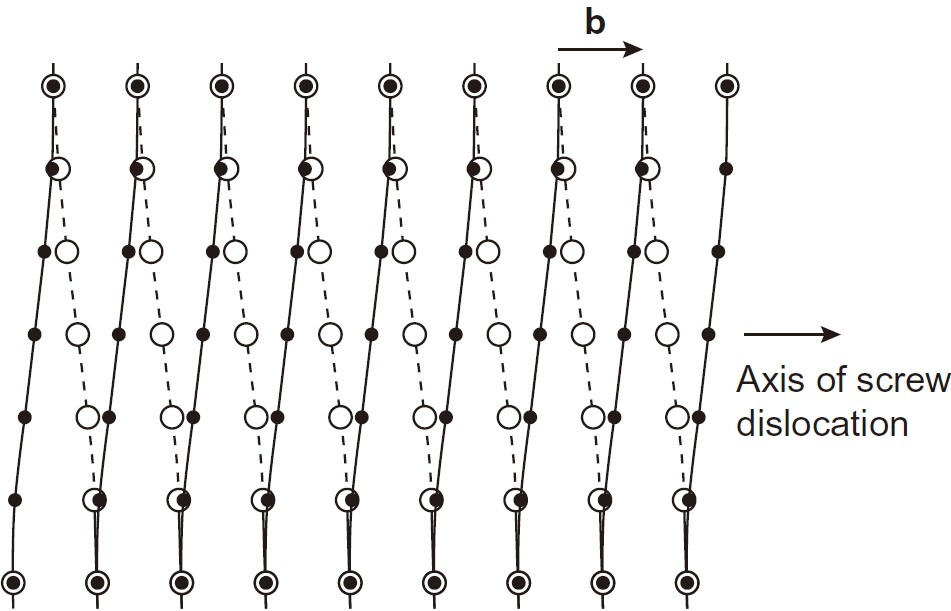
\includegraphics[width=0.5\textwidth]{fig/Arrangement_of_atoms_of_slip_of_screw_dislocation.jpg}
                    \caption{螺位错滑移时位错周围原子的动作。}
                    \label{螺位错滑移时位错周围原子的动作}
                \end{figure}

                对于混合位错,可以分解为螺位错和刃位错,因此运动方向也是两者的矢量合成方向。

                总而言之,位错的滑移过程是一个组态的传递,实际晶体中的位错滑出晶体后会在晶体表面造成台阶。
                对于位错的滑移可以得出以下结论:
                \begin{itemize}
                    \item 原子的迁移很小、所需要的力也很小,逐步推移、力在柏式矢量方向上要有分量;
                    \item 晶体错动$\vec{b}$后晶体内不存在畸变,与位错线的形状无关;
                    \item 移动方向不是由柏式矢量方向确定,而是永远与位错线垂直的方向,对于弯曲的位错线则沿其对应点的法线方向;
                    \item 刃型位错与螺型位错的滑移面、滑移方向、和台阶方向如\autoref{位错的滑移过程总结}所示。
                \end{itemize}

                \begin{table}[ht]
                    \centering
                    \caption{位错的滑移过程总结。}
                    \label{位错的滑移过程总结}
                    \begin{tabular}{@{}cccc@{}}
                        \toprule
                        位错类型 & 滑移面法线方向                & 滑移方向     & 台阶方向     \\ \midrule
                        刃位错  & $\vec{b}\times\vec{l}$ & 平行于切应力方向 & 平行位错线方向  \\
                        螺位错  & 密排面法线方向                & 垂直于切应力方向 & 垂直位错线方向 \\ \bottomrule
                    \end{tabular}
                \end{table}

                另外,刃型位错还存在一种特有的运动方式,也就是攀移。刃型位错本身如果垂直于它的滑移面运动,
                刃型位错的半薄片材料不是增长就是缩短,要实现这种运动,就需要原子的迁移来扩散质量。
                例如空位不断扩散到刃型位错,它的半薄片材料上的原子跳入空位,是的半薄片材料本身减缩,结果使
                刃型位错向上攀移一个原子间距。

                攀移的机制虽然也可以通过间隙原子的扩散,但是空位机制更为可能。攀移过程有原子的减少和增加,这
                与扩散有直接的关系,同时也与温度有关系,因为这是一个热激活过程,且其中存在体积变化,如果位错
                线不是整体攀移,还会造成割阶,如\autoref{刃型位错上的割阶}所示。
                \begin{figure}[ht]
                    \centering
                    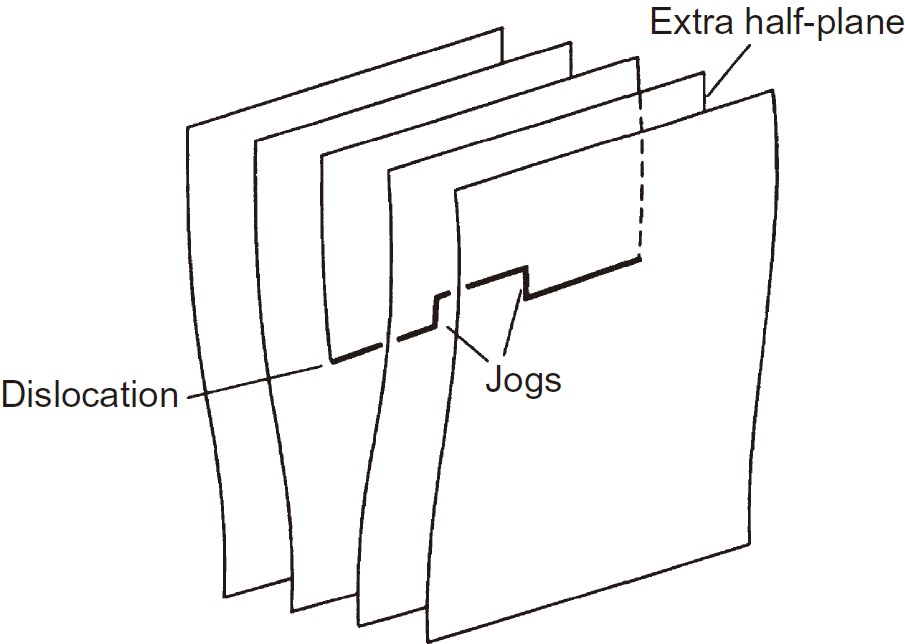
\includegraphics[width=0.5\textwidth]{fig/A_pair_of_jogs_on_an_edge.jpg}
                    \caption{刃型位错上的割阶。}
                    \label{刃型位错上的割阶}
                \end{figure}

            \subsection{位错运动与晶体变形}
            当位错滑出晶体后,会在晶体表面造成台阶,如果若干个位错滑出晶体,将会引
            起晶体的宏观变形,下面来分析一下晶体的宏观变形与位错滑移之间的关系。首先看
            一下单个位错的情况。如\autoref{刃型位错滑移造成的范型变形}所示,多个位错可以先
            叠加为一个位错$\vec{D}$。假设位错划过整个晶体扫过的面积为
            \begin{equation}
                A=l\cdot d,
            \end{equation}
            引起的变形为:
            \begin{equation}
                \gamma=\frac{D}{h}.
            \end{equation}
            如果位错只滑动了$\alpha d$,$0<\alpha<1$,位错扫过的面积为
            \begin{equation}
                A^\prime=\alpha l_2l_3,
            \end{equation}
            引起的变形为:
            \begin{equation}
                \gamma^\prime=\frac{\alpha D}{h}=\alpha\gamma.                
            \end{equation}
            \begin{figure}[ht]
                \centering
                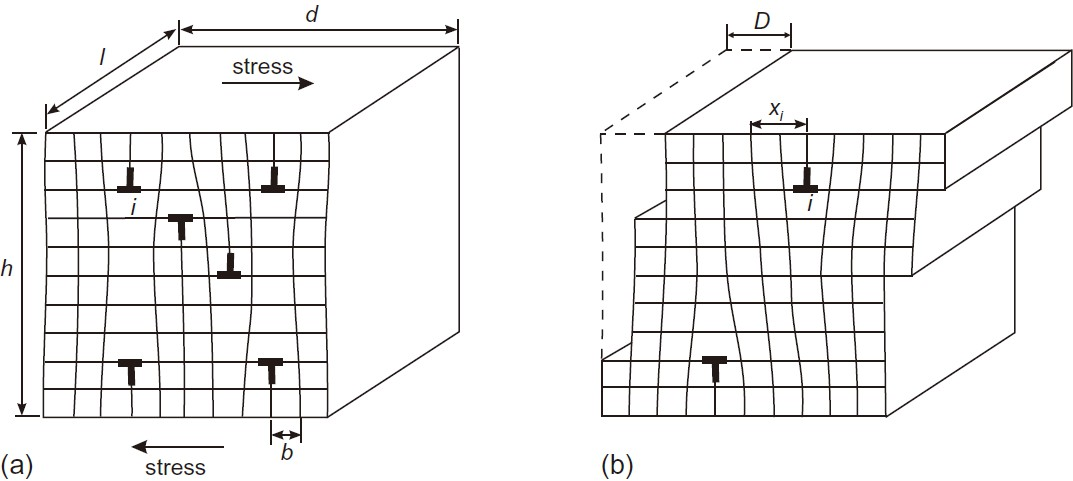
\includegraphics[width=0.7\textwidth]{fig/deformation_by_edge_dislocation.jpg}
                \caption{刃型位错滑移造成的范型变形。}
                \label{刃型位错滑移造成的范型变形}
            \end{figure}

            对于多个位错,采用面密度\index{位错!面密度}和体密度\index{位错!体密度}的方法来分析。面密度定义为
            单位面积上位错的露头数,而体密度定义为单位体积内位错的长度。因此如果若干个位错总长度为$L=\sum l_i$,
            平均移动距离为$S$,则扫过的总面积为$\sum l_i S=L\cdot S$,每根位错的平均滑移量为$\frac{L\cdot S}{A}\cdot D$,
            引起的总应变为
            \begin{equation}
                \gamma=\frac{LSD}{Ah}=\frac{LSD}{V}=\rho_v SD\label{刃型位错变形与体密度关系},
            \end{equation}
            其中$\rho_v$为位错的体密度,$V$为晶体体积,对于长方体的晶体可以也可有以下写法:
            \begin{equation}
                V=h(\cdot l\cdot d)=l\cdot(h\cdot d),
            \end{equation}
            代入\autoref{刃型位错变形与体密度关系},可得
            \begin{equation}
                \gamma=\frac{LSD}{V}=\frac{nl SD}{V}=\rho_s SD,
            \end{equation}
            其中$\rho_s$为位错的面密度。

            由于实际中位错的柏式矢量一般用$\vec{b}$表示,这里为了不产生冲突,才使用了$\vec{D}$,
            在之后的内容中,这一公式都会写作
            \begin{equation}
                \gamma=\rho Sb.
            \end{equation}

            由于刃位错在厚度方向分布不均匀,晶体会发生弯曲,如\autoref{晶体的范性弯曲}所示,上下两端弧的
            长度差为
            \begin{equation}
                \mathrm{AB}-\mathrm{CD}=(r+d)\theta-r\theta=\theta d,
            \end{equation}
            则晶体中的上半原子面数也就是位错数为
            \begin{equation}
                n=\frac{\theta d}{b},
            \end{equation}
            当晶体的厚度为$l_3$时,位错的体密度和面密度为
            \begin{align}
                \rho_v=\frac{\theta dl_3}{bV}=\frac{\theta dl_3}{b\theta rdl}=\frac{1}{br},\\
                \rho_s=\frac{\theta d}{b\theta rd}=\frac{1}{br}=\rho_v.
            \end{align}
            \begin{figure}[ht]
                \centering
                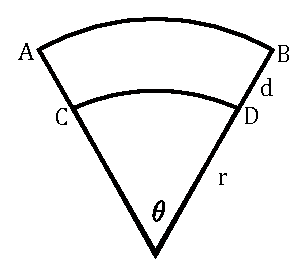
\includegraphics[width=0.5\textwidth]{fig/bending_of_crystal_for_dislocation.eps}
                \caption{晶体的范性弯曲。}
                \label{晶体的范性弯曲}
            \end{figure}

            \subsection{作用在位错上的力}
                在\autoref{subsection:点阵阻力}中,将点阵阻力定义为原子势的梯度,在这一节中,
                仍然使用这个定义,
                \begin{equation}
                    F=-\nabla U\label{位错力的定义},
                \end{equation}
                并用其分析位错运动中受到的滑移力、攀移力等。
                
                \subsubsection{滑移力}
                    假设位错的滑移面面积为$S$,位错线长度为$\xi$,滑动了$\dif l$,
                    位错的柏式矢量为$\vec{b}$,扫过的面积为$\xi\cdot\dif l$,产生的平均滑移量为
                    \begin{equation}
                        A=\frac{\xi\dif l}{S}\cdot b=\alpha b,
                    \end{equation}
                    滑移面受到的外力为
                    \begin{equation}
                        F=S\cdot\tau,
                    \end{equation}
                    外力所做的功为
                    \begin{equation}
                        \dif W=F\cdot A=\frac{S\tau b\xi\dif l}{S}=\tau bd\xi\dif l=\dif U,
                    \end{equation}
                    根据定义\autoref{位错力的定义}可得
                    \begin{equation}
                        F^{\prime}=\frac{\dif U}{\dif l}=\tau b\xi,
                    \end{equation}
                    令$\xi=1$,则有
                    \begin{equation}
                        F^{\prime}=\tau b.
                    \end{equation}

                    位错受到的滑移力有以下特点
                    \begin{itemize}
                        \item 力的方向垂直于位错线;
                        \item $\tau$必须在柏式矢量方向上有分量;
                        \item 滑移力为组态力,并不是位错附近原子实际受到的力。
                    \end{itemize}
                \subsubsection{攀移力}
                    假设一小部分的位错线$l$沿半原子面方向发生位移$s$,此时发生的体积变化为
                    \begin{equation}
                        \dif V=b\cdot l\times s=s\cdot b\times l,
                    \end{equation}
                    面积微元为$\dif S=\dif V/s$,受力为
                    \begin{equation}
                        F=\sigma_{yy}\dif S,
                    \end{equation}
                    发生攀移所做的功为
                    \begin{equation}
                        \dif W=F\cdot s=\sigma_{yy} s\dif S=\sigma_{yy}slb,
                    \end{equation}
                    假设位错的攀移力为$F_c$,此过程中做功为
                    \begin{equation}
                        \dif W=F_c\cdot l\cdot s,
                    \end{equation}
                    所以位错的攀移力为
                    \begin{equation}
                        F_c=-\sigma_{yy}\cdot b.
                    \end{equation}
                    
                    这一过程需要扩散,因此也需要热激活,因此攀移一般发生在较高的温度下。
                \subsection{位错攀移阻力和化学力}
                    假设一个原子所占的体积为$\Omega$,则填补$\dif V$的空隙需要$\dif V/\Omega$个
                    点缺陷,假设$\Omega=b^3$,所以原子数为
                    \begin{equation}
                        \dif n=\frac{ls}{b^2}.
                    \end{equation}

                    假设攀移阻力为$F_z$,则攀移形成体积$\dif V$所需的功为
                    \begin{equation}
                        W=\sigma_{yy}\cdot\dif V,
                    \end{equation}
                    需要的原子数为$\dif n=\dif V/\Omega$。

                    假设点缺陷形成能为$E_f$,则填补$\dif V$的形成能为
                    \begin{equation}
                        \dif n\cdot E_F=\frac{E_f ls}{b^2}=F_z\cdot s=-\sigma_{yy}lsb,
                    \end{equation}
                    因此有
                    \begin{equation}
                        F_z=\frac{E_f}{b^2}=-\sigma_{yy}b,
                    \end{equation}
                    因此空位形成能与应力的关系为
                    \begin{equation}
                        \sigma_{yy}=\frac{E_f}{b^3},
                    \end{equation}
                    一般来讲,空位形成能为
                    \begin{equation}
                        E_f=\frac{\mu b^3}{5}.
                    \end{equation}

                    如果晶体中存在过饱和空位,这时单位时间内体哦啊到位错上的空位数
                    就要超过离开的位错数,从而产生位错攀移的驱动力,这种里称为化学力。
                    假设在某一温度下,晶体的空位平衡浓度为$c_v$,而实际浓度为$c$,则空位的化学势,即
                    与一个空位消失与位错相关的自由能变化为
                    \begin{equation}
                        \mu_v=\frac{\partial F}{\partial n}=kT\ln\frac{c}{c_0},
                    \end{equation}
                    单位为错攀移单位距离时,所需的空位数为$1/b^2$,相应的自由能变化就被
                    定义为单位长度位错线所受的化学攀移力,即
                    \begin{equation}
                        F_c=\frac{1}{b^2}kT\ln\frac{c}{c_0}.
                    \end{equation}
                \subsection{位错的一般力公式}
                    $\dif l$的位错受到空间力场$\sigma$的作用,在滑移面A上运动$\dif s$
                    距离,此时的滑移面积为$\dif A=\dif l\cdot\dif s$。设$\vec{n}$为A面法线,
                    对应矢量为$(n_x,n_y,n_z)$,空间中一个面积元为
                    \begin{equation}
                        \dif A =n \cdot\dif A.
                    \end{equation}
                    
                    空间中的应力场包括三个正应力、六个切应力,用应力张量表示
                    \begin{equation}
                        \sigma=\begin{bmatrix}
                            \sigma_{xx}&\tau_{xy}&\tau_{xz}\\
                            \tau_{yx}&\sigma_{yy}&\tau_{yz}\\
                            \tau_{zx}&\tau_{zy}&\sigma_{zz}
                        \end{bmatrix}.
                    \end{equation}
                    则空间中任意斜面的总外力为
                    \begin{equation}
                        F=\sigma\cdot n\dif A,
                    \end{equation}
                    外力使该面移动b所做的功为
                    \begin{equation}
                        W=b\cdot\left( \sigma\cdot n\dif A \right)=b\left[ \sigma\cdot(\dif l\times\dif s) \right]\cdot\dif s,
                    \end{equation}
                    根据矢量叉乘的性质可以变成
                    \begin{equation}
                        W=\left( b\sigma\times\dif l \right)\dif s,
                    \end{equation}
                    设作用在位错上的力为$\dif F$,滑移矢量为$\dif s$,柏式矢量为$\vec{b}$,
                    则$\dif F$做功为
                    \begin{equation}
                        W=\dif F\cdot\dif s=\left( b\sigma\times\dif l \right)\dif s,
                    \end{equation}
                    因此
                    \begin{equation}
                        \dif F=b\sigma\times\dif l,
                    \end{equation}
                    如果令$t$为$\dif l$的单位向量,则可以写为
                    \begin{equation}
                        \dif F=b\sigma\times t.
                    \end{equation}
                    所以位错运动受力的特点为:
                    \begin{itemize}
                        \item[1] 受力方向总与位错线垂直;
                        \item[2] 位错受力与外力方向不一致。
                    \end{itemize}
                \subsection{位错像力}
                    在研究半无限大介质中的一个位错时,这个位错和介质的表面平行,距离表面的距离为$l$,
                    根据位错应力场计算的结果在表面存在应力,但是实际上表面的总应力应当为零,这就需要在
                    以表面为对称的位置上存在一个想象的柏式矢量相反的位错,这样才能满足边界条件。

                    实际上产生这项吸引力的原因是位错倾向于接近自由表面以松弛其弹性应变能。
                    按照组态力的概念我们用一个力来描述系统自由能降低的趋势,这个力就是像力。
                    更为具体的分析结果可以通过\href{https://brilliant.org/wiki/greens-functions-in-physics/}{Green函数}来分析。
        \section{位错与晶体缺陷间的相互作用}
            由于晶体中的位错具有长程应力场,当晶体中同时存在有其他晶体缺陷时,同样
            地这些缺陷改变了原子的规则排列,从而在晶体中引入了畸变,它们之间就会发生相
            互作用。本节主要讨论位错与其它位错以及点缺陷之间的相互作用。
            
            晶体之间存在大量的位错,因此,各个位错之间会由于应力场的作用产生相互长程应力
            作用,当两个位错相遇时,两者之间还会产生短程的相互作用。首先来分析长程应力场
            之间的相互作用。
            \subsection{弹性应力场之间的相互作用}
                    晶体中常常包含有很多位错,它们的弹性应力场之间发生干涉和相互作用,
                    并且将影响到位错的分布和运动。直接处理任意分布大量位错之间的相互作用是
                    非常困难的,有效的方法是从最简单、最基本的情况入手。

                    首先讨论一堆螺位错之间的相互作用,在坐标原点和$(r,\theta)$处有一对平行于
                    $z$轴的同号螺型位错,柏式矢量分别为$\vec{b}_1$和$\vec{b}_2$。位错$\vec{b}_1$
                    在$(r,\theta)$处的应力场为
                    \begin{equation}
                        \sigma_{\theta,z}=\frac{\mu b_1}{2\pi r},
                    \end{equation}
                    对于位错$\vec{b}_2$来说,此应力分量作用在它的滑移面上且平行于它的柏式矢量,即
                    ,满足滑移的条件,按照滑移力的计算,位错$\vec{b}_2$受到的力为
                    \begin{equation}
                        F=\frac{\mu b_1 b_2}{2\pi r}\label{两个螺型位错之间的作用力},    
                    \end{equation}
                    这个力要求它沿两位错连线方向向往外运动,里的大小随两位错间距的增加而降低。
                    同理,$\vec{b}_1$也受到$\vec{b}_2$大小相等方向相反的力。如果俩个螺位错的符号相反,
                    则就会变为吸引力,这与两条通电导线的作用相似。
                    
                    对于平行滑移面两个刃型位错,两者的位错线与$z$轴平行,柏式矢量分别为$\vec{b}_1$和$\vec{b}_2$。
                    根据\autoref{刃位错的x主应力}和\autoref{刃位错的切应力},$\vec{b}_2$所在处$\sigma_{xx}$使
                    其受到攀移力,$\tau_{yx}$使位错$\vec{b}_2$受到滑移力,分别为
                    \begin{align}
                        F_x&=\sigma_{yx}b_2=\frac{\mu b_1b_2}{2\pi(1-v)}=\frac{z(x^2-y^2)}{(x^2+y^2)^2}\label{两个刃型位错之间的相互作用力},\\
                        F_y&=-\sigma_{xx}b_2=\frac{\mu b_1b_2}{2\pi(1-v)}=\frac{y(3x^2+y^2)}{(x^2+y^2)^2}.
                    \end{align}

                    对得到的结果分析可知,$F_y$与$y$同号,也就是当位错$\vec{b}_2$在位错$\vec{b}_1$滑移面
                    上边时,受到的攀移力$F_y$指向上,在滑移面下边时,受到的攀移力指向下,所以沿$y$轴方向两
                    位错是互相排斥的。然而当$x^2<y^2$时$F_x$指向外,所以两位错沿$x$方向相互排斥,当$x^2<y^2$
                    时,$F_x$指向内,所以两位错沿$x$轴方向互相吸引,如\autoref{两刃型位错在x轴方向上的相互作用}
                    所示。在$x=0$以及$x=\pm y$的位置,$F_x$虽然等于零,但是这两种位置不同。$x=0$为稳定平衡位置,
                    \begin{figure}[ht]
                        \centering
                        
\includegraphics[width=0.5\textwidth]{fig/force_of_edge_dislocations_along_x_axis.eps}
                        \caption{两同号刃型位错在$x$轴方向上的相互作用。}
                        \label{两刃型位错在x轴方向上的相互作用}
                    \end{figure}
                    因为当位错$\vec{b}_2$稍微偏离这个位置时,会受到回复的力,而$x=\pm y$是不平衡位置,
                    $\vec{b}_2$发生偏离时,受到的力使其偏离的更远。所以相同符号的刃型位错沿着
                    与它们柏式矢量相垂直的方向排列起来是稳定的\footnote{这样的位错排列会形成一种晶粒边界。}。
                    加入两个位错的符号相反,它们之间的作用力的方向也要改变,而$x=0$变为不稳定的平衡位置,
                    $x=\pm y$变为稳定的平衡位置。符号相反的两个位错依靠弹性相互作用在\ang{45}方向上彼此
                    束缚在一起,构成通常所围的位错偶极子。

                    当两个位错相互平行,分别为纯螺型和纯刃型,由于螺位错的应力场没有使刃位错受力的应力分量,
                    刃位错的应力场也没有使螺位错受力的应力分量,所以两个位错没有相互作用。

                    对于具有任意柏式矢量的两个平行的直线位错,可以把每个位错都分解为刃型分量和螺型分量,
                    然后依次计算两个螺型分量和两个刃型分量之间的相互作用,并且叠加起来,就得到了任意两个
                    位错之间的相互作用,对所得记过可以近似地归纳为:若柏式矢量夹角小于$\frac{\pi}{2}$,
                    则两个位错互相排斥,若柏式矢量夹角大于$\frac{\pi}{2}$,则两个位错互相吸引。
            \subsection{位错塞积}
                现在我们开始研究位错集群在外加应力、障碍以及集群内部的相互作用力下的平衡问题。晶体材料中通常有许多位错,
                在外加应力作用下在滑移面上滑动。假如滑移面上遇到强的障碍物,
                领先的位错不能越过障碍,这样就会形成由许多位错组成的塞积群。
                实际材料中的晶界或第二相硬颗粒都是可以产生位错塞积群的障碍物。

                在分切应力作用下,由同一位错源放出的位错在障碍前受到阻碍,这些位错就在障碍前排列起来,
                这种位错组态称为塞积群,如\autoref{实际晶体中的塞积群}所示。

                位错塞积群在受力上可以分为三类:
                \begin{itemize}
                    \item[1] 领先位错受到的障碍物的作用;
                    \item[2] 各个位错之间的相互作用;
                    \item[3] 外加应力作用。
                \end{itemize}

                对于外力具体的求解过程比较复杂,这里只给出主要结果。领先位错前的切应力
                为
                \begin{equation}
                    \tau^{\prime}=n\tau,
                \end{equation}
                此式表明,当有$n$个位错被外加切应力$\tau$推向障碍物时,位错塞积群的前端将
                产生$n$倍与外力的应力集中。

                塞积群的长度为
                \begin{equation}
                    L=xn=\frac{\vert A\vert \pi^2}{8n\tau}(n-1)^2,
                \end{equation}
                与切应力$\tau$成反比。
                \begin{figure}[ht]
                    \centering
                    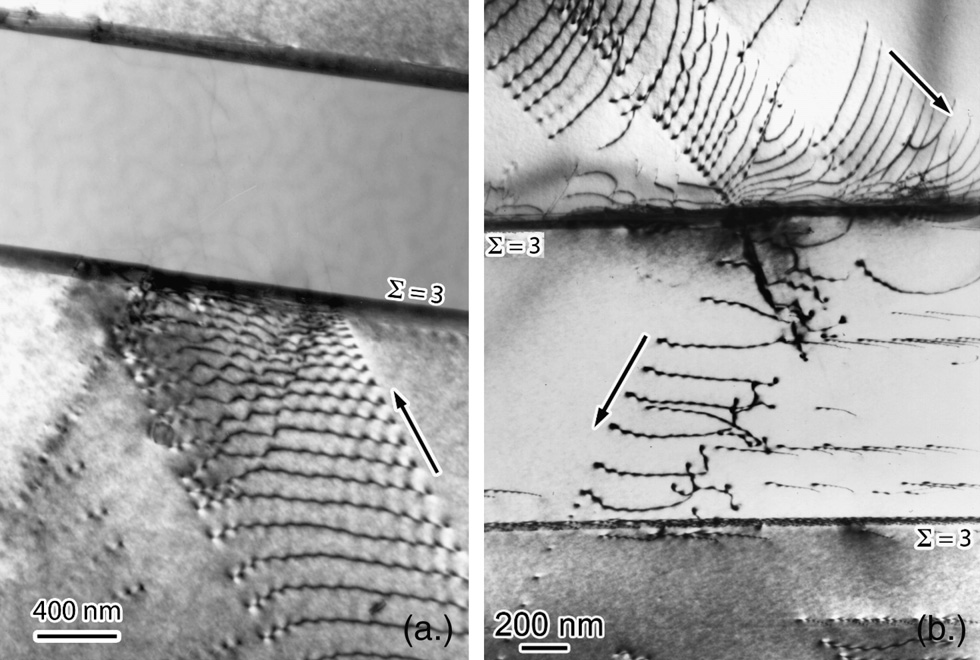
\includegraphics[width=0.7\textwidth]{fig/pile_up_groups_&_slip_transmit_twin_boundary.jpg}
                    \caption{层错能较低的材料的孪晶界的TEM原位照片\cite{SANGID2011283},(a)为滑移被孪晶界阻碍,形成位错塞积群,(b)为加载力过大时,滑移进入孪晶界。}
                    \label{实际晶体中的塞积群}
                \end{figure}
            
            \subsection{位错交割}
                在晶体的范性形变过程中会产生不同滑移面上位错相交截的现象.这里牵涉到位
                错间的弹性相互作用以及近程相互作用。下面分别考虑这两种相互作用:
                \begin{itemize}
                    \item[1] 弹性相互作用:设不同滑移面上的位错线相交,且夹角大于$\frac{\pi}{2}$,由于弹性相互作用,两个位错可以合成新的位错线段,以降低弹性能;
                    \item[2] 位错的中心区可能产生近程的相互作用。
                \end{itemize}

                对于在滑移面上运动的位错来说,穿过此滑移面的其它位错称为林位错\index{林位错}。
                林位错会阻碍位错的运动,但是若应力足够大,滑动的位错将切过林位错继续前进。位错相互切割的过程称为位错交割\index{位错交割}。

                \begin{figure}[ht]
                    \centering
                    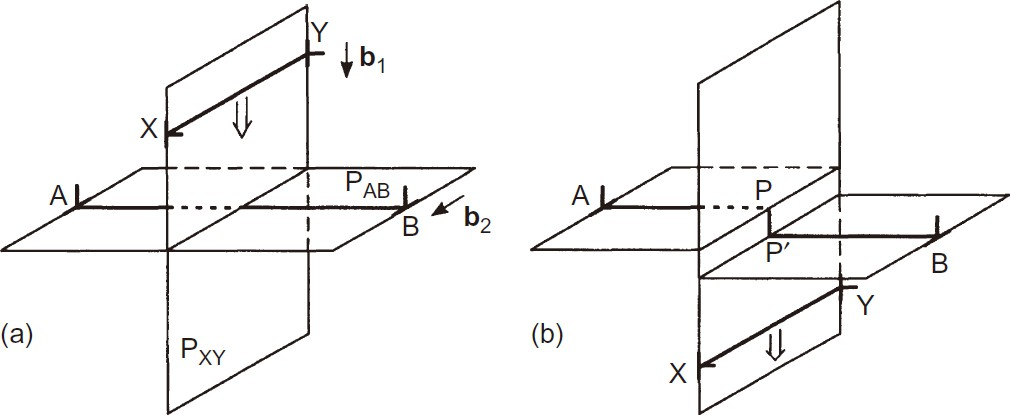
\includegraphics[width=0.7\textwidth]{fig/Intersection_of_edge_dislocations_with_Burgers_vectors_at_right_angles_to_each_other.jpg}
                    \caption{两个柏式矢量垂直的刃位错的相互作用\cite{HULL2011137},(a)位错xy沿滑移面$P_{\mathrm{xy}}$移动,并切过$P_{\mathrm{AB}}$面的AB位错,(b)为
                        xy已经切过AB,并且产生了$\mathrm{PP}^{\prime}$割阶。}
                    \label{两个垂直的刃位错的相互作用}
                \end{figure}
                
                \autoref{两个垂直的刃位错的相互作用}表示两个刃位错的相互交割,$\mathrm{P}_{\mathrm{AB}}$面
                的位错保持不动,而$\mathrm{P}_{\mathrm{xy}}$面的位错向下移动,柏式矢量为$\vec{b}_1$,当$\vec{b}_1$
                扫过时$\mathrm{P}_{\mathrm{AB}}$面两侧发生了相对位移$\mathrm{PP}^{\prime}$,方向和大小与
                取决于$\vec{b}_1$。由于位错的连续性,即位错不能在晶体内部中断,$\mathrm{PP}^{\prime}$必然是
                一小段位错,又由于柏式矢量的守恒性,它的柏式矢量也必然是$\vec{b}_2$。这一小段位错$\mathrm{PP}^{\prime}$
                称为位错割阶。产生割阶需要能量供给,所以交割过程对位错运动是一种阻碍。粗略估计,
                割阶能量的数量级为$\frac{\mu b^3}{10}$,对于一般金属约等于十分之几个电子伏特。

                其次考虑一个刃型位错与一个螺型为位错的交割,如\autoref{刃型位错与螺型位错交割}所示,图中螺型位错的柏式矢量为
                $\vec{b}_2$,按照螺型位错的特点,被它贯穿的一组晶面组成一个螺旋面。另一个位错的柏式矢量为$\vec{b}_1$,
                是一个刃型位错,其滑移面恰好是螺型位错$\vec{b}_2$的螺旋面。当位错$\vec{b}_1$切过螺型位错后,
                变成了分别位于两层晶面上的两段位错,两者的连线$\mathrm{PP}^{\prime}$也是一个位错割阶,大小
                个方向等于螺型位错的柏式矢量$\vec{b}_2$,而其自身的柏式矢量与刃型位错相同,仍然是一段刃型位错,
                割阶随位错$\vec{b}_1$一同向前的运动也是滑移。
                \begin{figure}[ht]
                    \centering
                    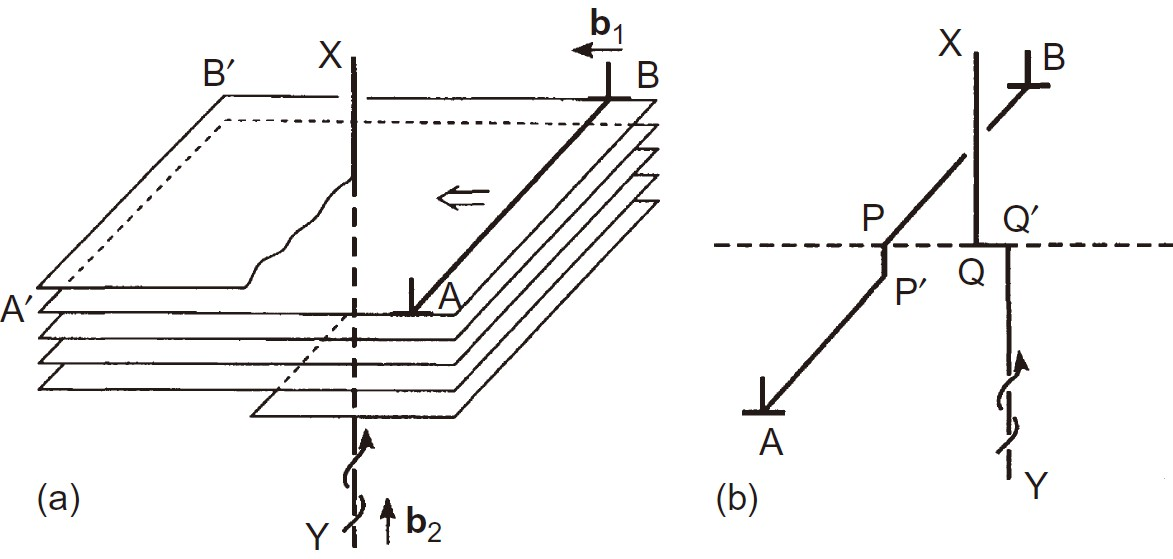
\includegraphics[width=0.7\textwidth]{fig/Intersection_of_an_edge_dislocation_with_a_right-handed_screw_dislocation.jpg}
                    \caption{刃型位错$\mathrm{AB}$与垂直的右螺型位错$\mathrm{XY}$的相互作用,(a)$\mathrm{AB}$在滑移面移动切割$\mathrm{XY}$,
                        由于螺位错使晶体螺旋上升一层,因此当切过螺位错,到达$\mathrm{A}^{\prime}\mathrm{B}^{\prime}$时,$\mathrm{AB}$不再处于
                        同一个平面,也就是在(b)中的割阶$\mathrm{PP}^{\prime}$。}
                    \label{刃型位错与螺型位错交割}
                \end{figure}

                一般情况下,两个位错交割时,每个位错上都要产生一小段位错,它们的柏式矢量与其本身相同,但是
                大小和方向取决于另一位错的柏式矢量。当交割产生的小段位错不在所属的位错的滑移面时,则称为位错割阶,且所有的割阶都是刃型位错,
                如果小段位错位于所属位错的滑移面上,则相当于位错扭折\index{位错扭折}。

            \subsection{位错与溶质原子之间的相互作用}
                \subsubsection{弹性交互作用}
                    由于位错具有长程应力场,因此可以与溶质原子产生的畸变发生相互作用,这种作用称为弹性交互作用。

                    对于刃型位错来说,假设以位错核心为原点建立极坐标系,假设晶体中的一个基体原子的半径为$r_0$,
                    在$(r,\theta)$存在一个半径为$r_0(1+\varepsilon)$的小球,相当于将一个体积与基体原子不同的
                    溶质原子放入晶体的空位,其中$\varepsilon$称为错配度,表示溶质原子与基本原子的差别的大小。
                    在此过程中,外力反馈位错应力场所作的共就是位错与溶质原子的交互作用能。由于小球在周围介质中
                    引起的位移垂直于球面,位错的应力场中只有正应力分量$\sigma_{xx}$,$\sigma_{yy}$和$\sigma_{zz}$
                    做功,平均值为
                    \begin{equation}
                        \sigma=\frac{1}{2}\left( \sigma_{xx}+\sigma_{yy}+\sigma_{zz} \right),
                    \end{equation}
                    在位移$\varepsilon a$的过程中,位错应力场所做的功为$4\pi\sigma\varepsilon r_0^3=\sigma\Delta V$,
                    $\Delta V=4\pi\varepsilon r_0^3$为溶质原子与基体原子的体积差。从而位错与溶质原子的相互作用能为
                    \begin{equation}
                        U=-\frac{1}{2}\left( \sigma_{xx}+\sigma_{yy}+\sigma_{zz} \right)\Delta V,
                    \end{equation}
                    把刃型位错应力场\autoref{刃位错的x主应力}、\autoref{刃位错的y主应力}和\autoref{刃位错的z主应力}代入上式,得到
                    \begin{equation}
                        U=A\cdot\frac{\sin\theta}{r},A=\frac{\mu b}{3\pi}\frac{1+v}{1-v}\Delta V,
                    \end{equation}
                    其中$r$和$\theta$代表溶质原子的坐标位置。

                    上式表明,当$\Delta V>0$,在$0<\theta<\pi$处,$U$为正,在$\pi<\theta<2\pi$处,$U$
                    为负。当$\Delta V<0$时则相反。平衡状态要求相互作用能最小,所以,比集体原子大的置换式溶质
                    原子和间隙原子将被位错的压缩区排斥,被位错的膨胀区吸引,而比基体原子小的置换式溶质原子和
                    空位的移动趋势恰好相反。

                    由于溶质原子与位错有相互作用,若时间和温度允许,它们将向位错附近聚集,形成科垂耳气团\index{科垂耳气团},
                    使位错的运动受到限制。因为在这种情况下,推动位错运动,或者首先挣脱气团的束缚,或者拖着气团一起前行,
                    无论如何都要做更多的功,这对应着拉伸曲线中的上屈服点。

                    对于螺位错来说,则没有弹性相互作用,这是因为螺位错的应力场只有切应力分量,二溶质原子产生的畸变又被
                    假定为球形对称,但是一旦畸变不再是球形,螺位错也会与溶质原子发生相互作用\footnote{比如体心立方铁晶格中的碳原子或氮原子。}。
                    这种相互作用有时称为史诺克气团\index{史诺克气团}。

                \subsubsection{模量相互作用}
                    设溶质原于大小和基体原于基本一样,但它的弹性不同,由此而产生的交互作用就是模量交互作用。
                    我们在这里仅做定性的分析。首先假定溶质原子比基体硬一些,即切变模量大一些。当一个螺型位错移近这个“硬点”的时候,
                    通过它的切应力对这个硬点施以变形的功不同于没有这个硬点而为基体时的变形功。
                    这个功的差额就是模量交互作用能的量度。在极端情况下,设溶质原子很硬,很难变形,
                    这种原子将抗拒螺型位错向它移近;若溶质原子比基体软一些,情况相反,
                    原子倾向于靠近位错,位错由这个软点拉出去,需要额外的功。刃型位错和螺形位错不同,
                    前者除了它的切应力对溶质原子施加切变以外,还可以通过它的正应力对溶质原子施加正向的变形。
                    刃型位错和溶质原子之闻也有模量交互作用。
                \subsubsection{化学相互作用}
                    以上讨论的都是全位错和溶质原子通过位错的应力场和溶质原子产生的体膨胀或畸变发生作用。现在阐述另一种不同的作用,全位错分解为不全位错,
                    ,其间有层错,在层错区溶质原子的浓度(平衡时)应该不同于基体中的溶质浓度。
                    这种作用首先被Suzuki所认识,称为化学作用。
                    当位错运动时,这种不均匀分布的溶质原子也将随位错移动,因此这种组态通常称为Suzuki气团(铃木气团)\index{铃木气团}。

        \section{位错的增殖}
            \subsection{位错起源}
                根据理论计算,位错的能量很大,除非晶体受到的应力基金理论切变强度,说明位错不是靠热激活
                能产生的,因此位错不会在晶体中均匀形核。位错出现的位置基本有以下几种:
                \begin{itemize}
                    \item 应力集中的位置可能形成位错;
                    \item 在不均匀变形中可能产生位错;
                    \item 过饱和的空位凝胶成空位片,空位片的坍塌导致位错环形成;
                    \item 杂质分凝、偏析,凝固后晶体成分与凝固之前不同,造成点阵常数不同,累计结果形成位错;
                    \item 晶体中沉淀无或夹杂无在周围基体中产生较大应力,导致位错产生;
                    \item 结晶过程中正在生长的两部分晶体相遇,如果两者的位相有轻微差别,在结合的位置就会形成位错。
                \end{itemize}
            \subsection{位错增殖}
                研究发现,退火金属的位错密度在$\SI{1e6}{\cm^{-2}}$左右,而冷变形金属的位错密度会急剧增加到
                \SI{1e12}{\cm^{-2}}左右,这说明在变形过程中存在位错密度的增殖过程,对于这一过程的解释,
                以Frank-Read 源\index{Frank-Read源}理论最为简洁。

                设想晶体中有一段位错线两端被钉住,在应力作用下,位错线由于滑移而弯曲,二位错所受
                作用力恒与位错相垂直,则位错的发展情况如\autoref{Frank-Read源}所示。
                \begin{figure}[ht]
                    \centering
                    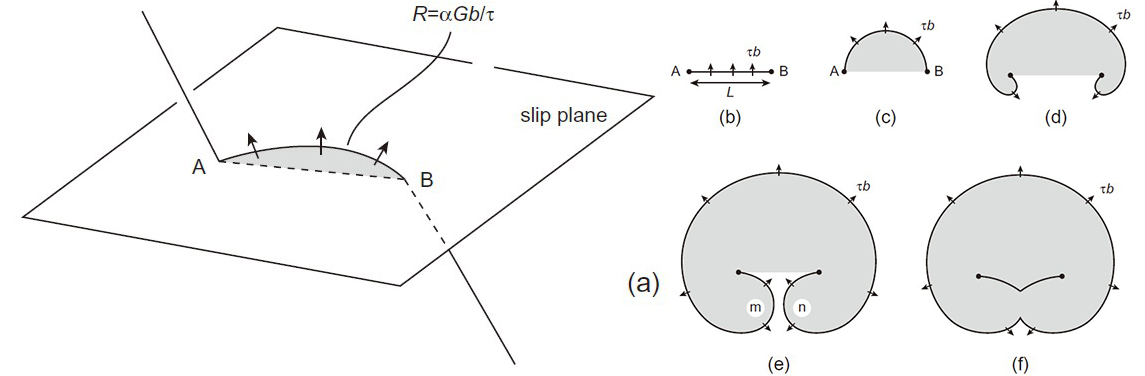
\includegraphics[width=0.8\textwidth]{fig/Frank_read_sources.jpg}
                    \caption{Frank-Read位错源图示。}
                    \label{Frank-Read源}
                \end{figure}
                当弯曲的线段相互靠近时。可以相互抵销,形成一闭合的位错圈和一段短线.这样的过程可以反复进行下去,
                源源不断地产生新的位错圈.当位错圈和晶体表面相截,就形成了台阶,这就是显微镜中所观察到的滑移线.
                当更多的位错圈和表面相交,中央部分的台阶逐渐变高,并向两侧伸展。

                下面进一步讨论为了开动位错源需要多大的应力,为此首先考虑一段弧形位错在滑移力和线张力的
                共同作用下的平衡。设想滑移面上的一端微元位错线$ab$在滑移力$F_\tau$和线张力的共同作用下到达
                平衡。平衡时,位错线$ab$的张角为$\delta\theta$,曲率半径为$R$,如\autoref{一段弧型位错的平衡}
                所示。根据静力学
                \begin{figure}[ht]
                    \centering
                    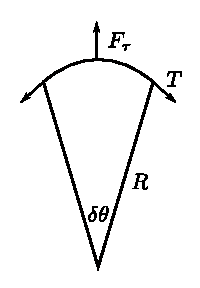
\includegraphics[scale=1]{fig/balance_of_FR_source.eps}
                    \caption{一段弧形位错的平衡。}
                    \label{一段弧型位错的平衡}
                \end{figure}
                \begin{equation}
                    2T\sin\frac{\delta\theta}{2}=F_\tau R\delta\theta,
                \end{equation}
                考虑到$\delta\theta$为无穷小,可以简化为
                \begin{equation}
                    2T\frac{\delta\theta}{2}=F_\tau R\delta\theta,
                \end{equation}
                或
                \begin{equation}
                    F_\tau=\frac{T}{R},
                \end{equation}
                将$F_\tau=\tau b$和$T=\frac{1}{2}\mu b^2$代入上式,得到
                \begin{equation}
                    \tau=\frac{\mu b}{2R}\label{线张力和切应力平衡条件},
                \end{equation}
                此式表面,当位错弧线达到平衡时,外加应力与弧线的曲率半径成反比,即位错曲率半径越小,
                要求与之相平衡的力越大。

                在\autoref{Frank-Read源}中,位错线AB弯曲之后,需要一定大小的切应力与之平衡,
                曲率约到,相平衡的切应力也越大。当位错线称为半圆形时,曲率达到了最大值,需要的切应力
                也为最大。可见,一个Frank-Read位错源受到适当切应力作用时,就开始运动和弯曲。
                起初为了弯曲能继续进行,所需的应力越来越大,直到位错完成半圆形,相应的的应力达到最大值,
                此后位错向外膨胀,曲率开始缩小,所需的应力也减小。因此位错开动的力取决于\autoref{Frank-Read源}
                中的(c)图对应的状态,此时的切应力为临界应力,\autoref{线张力和切应力平衡条件}可得临界切应力为
                \begin{equation}
                    \tau_c=\frac{\mu b}{2R}=\frac{\mu b}{l},
                \end{equation}
                其中$l$为位错线$AB$的长度,假设$l$长为\SI{1e-4}{\cm},$b$长度为\SI{1e-8}{\cm},
                对应的切应力为$10^{-4}\mu$,这和实际晶体的屈服强度接近。

                \begin{figure}[ht]
                    \centering
                    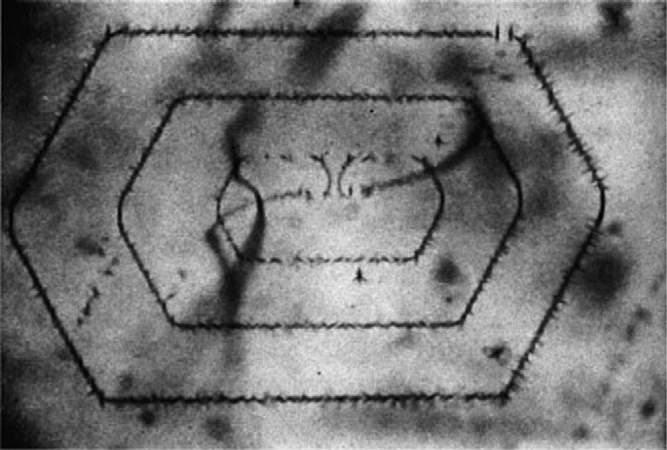
\includegraphics[width=0.7\textwidth]{fig/Frank_Read_source_in_a_silicon_crystal.jpg}
                    \caption{硅晶体中的Frank-Read位错源,通过缀饰法在硅晶体中显示出来的\cite{Dash1958}。}
                    \label{硅晶体中的Frank-Read位错源}
                \end{figure}

                \autoref{硅晶体中的Frank-Read位错源}是一个典型的位错源照片\cite{Dash1958},这个位错元正在释放位错环的时候被缀饰
                质点固定住了,由于硅是共价键晶体,错排能垒很高,所以位错线表现出明显的取向性。
        \section{实际晶体中的位错}
            前面我们讨论的位错的各种情况都是基于一个前提,以简单立方为例,而并未联
            系到晶体的具体结构,同时位错的柏氏矢量均为一个原子间距。但是在实际晶体中由
            于其具有不同的点阵类型,例如面心立方,体心立方等,其位错类型也会发生变化。
            首先我们定义全位错为柏氏矢量等于点阵矢量的位错,所以前面我们讨论的问题均是
            基于全位错\index{全位错}来考虑的。
            
                许多金属属于面心立方结构,这样的金属晶体的范性形变和晶体中的位错结构有
                密切关系,面心立方晶体中位错结构比上面经常作为例子的简单立方晶体中的位错
                复杂得多。设面心立方结构单位晶胞边长为$a$,点阵矢量$a$为$\langle110\rangle/2$类型,
                通常简写为$\frac{1}{2}\langle110\rangle$,也是最短的点阵矢量。所以面心
                立方晶体位错的柏式矢量最可能为$\frac{1}{2}\langle110\rangle$。之前证明
                位错的能量与$b^2$成正比,所以以$\frac{1}{2}\langle110\rangle$为柏式矢
                量的位错的应变能低于以$\langle100\rangle$为柏式矢量的位错能量,这就是面心立方
                结构没有$\langle100\rangle$位错的原因,而$\frac{1}{2}\langle110\rangle$为
                面心立方结构的单位位错。

                既然位错的应变能与位错的$b^2$成正比,因此一般来讲,最稳定的位错的柏式矢量应该为晶体的
                最短平移矢量。比如简单立方中的$\langle100\rangle$,面心立方中的$\frac{1}{2}\langle 110 \rangle$,
                体心立方中的 $\frac{1}{2}\langle 111 \rangle$,密排六方中的 $\frac{1}{3}\langle 11\bar{2}0 \rangle$
                和 $\langle 0001 \rangle$。

            \subsection{面心立方晶体中的位错和层错}

                对于面心立方来说, $\frac{1}{2}\langle 110 \rangle$型全位错和可以进一步分解,分解
                产生的柏式矢量小于点阵初基矢量,因而称为偏位错\index{偏位错}。在讨论偏位错之前,最好
                先了解堆垛层错。堆垛层错是一种面缺陷,由于讨论偏位错的需要,把它放在这里来介绍。

                \begin{figure}[ht]
                    \centering
                    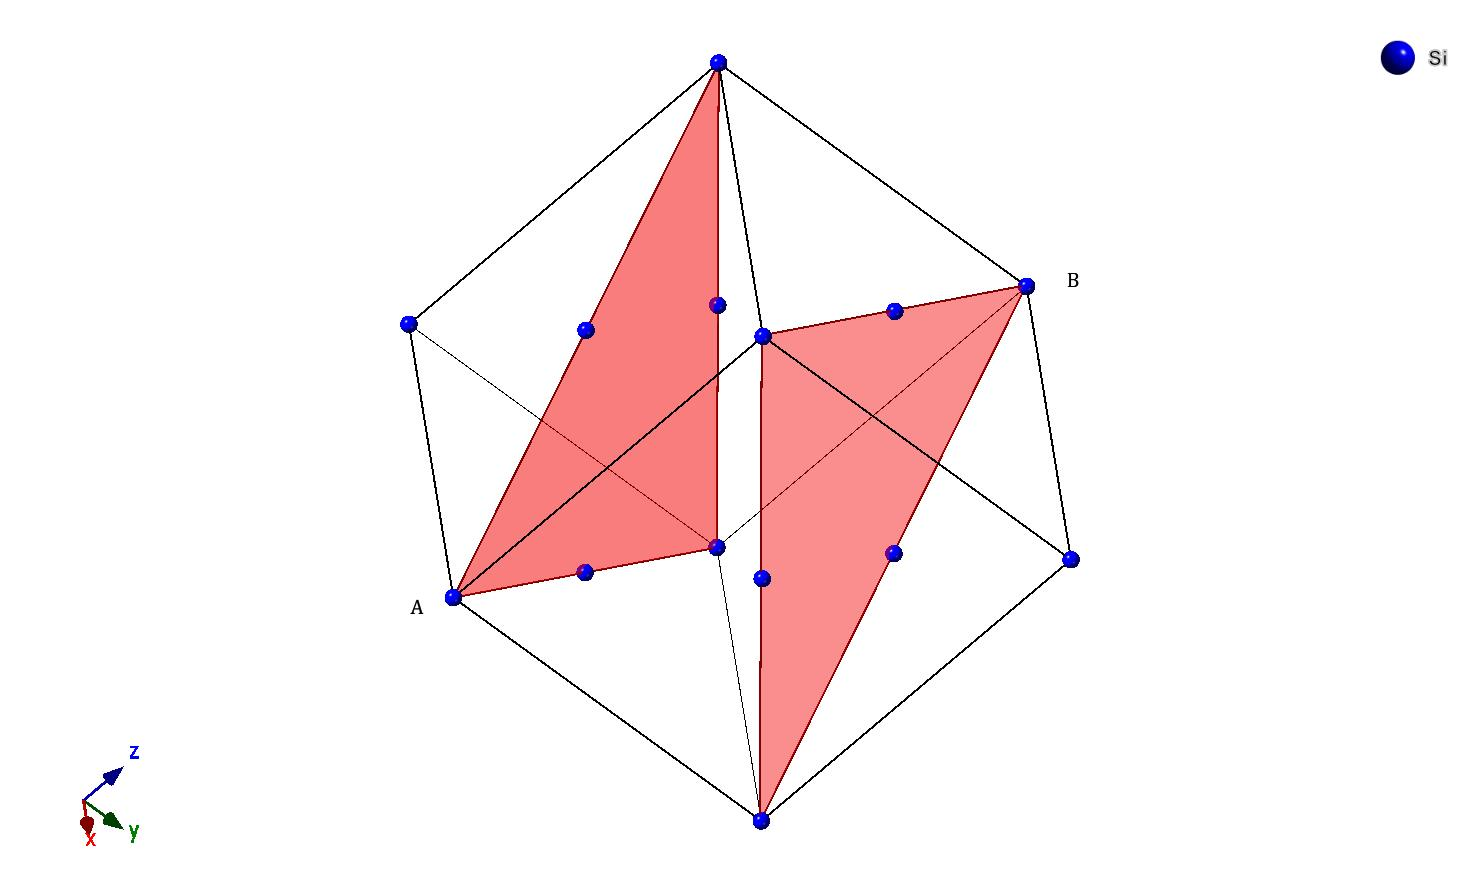
\includegraphics[width=0.5\textwidth]{fig/fcc_111.jpeg}
                    \caption{面心立方晶体单位晶胞以及$(111)面$。}
                    \label{面心立方晶体单位晶胞以及111面}
                \end{figure}
                
                \autoref{面心立方晶体单位晶胞以及111面}画出来面心立方晶体单胞内的两个相邻的$(111)$面,如果晶体上的原子
                简化成相切的小球,并且投影到$(111)$面上,则得到\autoref{面心立方111面堆垛}。三个相邻的$(111)$
                面的原子中心投影位置不同,为了区别,分别记作A、B、C,三个面也叫做A、B、C面。
                \begin{figure}[ht]
                    \centering
                    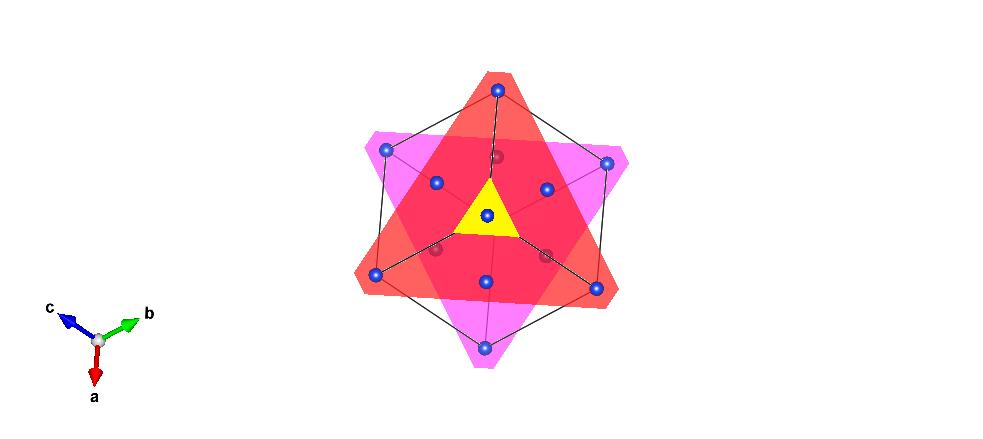
\includegraphics[width=0.7\textwidth]{fig/pile_up_of_planes_of_fcc_crystal.jpg}
                    \caption{面心立方的$(111)$堆垛情况。}
                    \label{面心立方111面堆垛}
                \end{figure}

                由\autoref{面心立方111面堆垛}可知,$(111)$面的堆垛规律为
                \begin{equation}
                    \cdots\cdots ABCABCABC\cdots\cdots 
                \end{equation}
                由于晶体的对称性,$(111)$面这种排列规律自然可以推广到所有的$\left\{ 111\right\}$
                晶面中去。

                晶面的正常堆垛次序被破坏时,就要出现堆垛层错或简称层错\index{层错}
                的晶格缺陷。面心立方晶体$\left\{ 111\right\}$面两种基本类型的层错
                可以表示为
                \begin{equation}
                    \cdots\cdots ABCACABC\cdots\cdots \label{面心立方层错形式1}
                \end{equation}
                和
                \begin{equation}
                    \cdots\cdots ABCACBCABC\cdots\cdots \label{面心立方层错形式2}
                \end{equation}
                \autoref{面心立方层错形式1}相当于从正常堆垛次序中抽掉一层晶面,因而称为
                抽出型层错\index{抽出型层错},层错中心位置位于缺少的晶面上;\autoref{面心立方层错形式2}
                相当于在正常堆垛次序中加入一层额外晶面,因而称为插入型层错\index{插入型层错},
                层错中心位置位于插入的晶面上。

                堆垛层破坏了晶体的完整性,是一种晶格缺陷,引起晶体能量的升高。与单位面积
                堆垛层错相联系的能量称为层错能\index{层错能}。从\autoref{面心立方层错形式1}
                和\autoref{面心立方层错形式2}可以看出,层错仅仅破坏了原子的次近邻关系,并
                没有破坏原子的最近邻关系,也即在层错处,只有从连续三层原子面的关系才能
                发现与正常堆垛次序的差别,如果仅仅取出相邻的两个原子面来看,无法观察到层错。
                因此层错虽然具有能量,但是与最近邻原子关系受到破坏的一般晶粒编辑的界面能相比,
                层错能要小得多。虽然目前理论计算层错能尚未解决,但是有一些估计层错能的实验方法。
                
                在薄晶体的电子显微镜衍衬法中,层错会引起特殊的干涉条纹,根据这种效应,
                可以之间看到层错能较小的晶体和合金中的层错。

                如果层错不贯穿整个晶体,而是中止余晶体内部,它就有一个边界线,如\autoref{Frank_partial_dislocation}
                所示。为了确定层错边界线的性质,围绕它作一个柏式回路。要注意回路的期待你应该选在层错面上,
                否则,回路在中途会穿过层错,造成困难。经过用柏式回路方法分析,可以证明上述层错都是具有 
                $\frac{1}{2}\langle 111 \rangle$小于面心立方晶体的初基矢量,所以这种类型的位错称为
                Frank偏位错\index{偏位错!Frank偏位错}。一般称与抽出型层错相联系的偏位错为负Frank偏位错,
                而与插入型层错相联系的偏位错被称为正Frank偏位错。Frank偏位错的柏式矢量与位错线垂直,因而总是
                刃型,但是它们不能滑移,因为如果滑移,就要离开所在的$(111)$面,并且在经过的路径上造成严重的
                原子错排,但是它们可以通过吸收或放出点缺陷在包含它们的$(111)$面作攀移运动。
                \begin{figure}[ht]
                    \centering
                    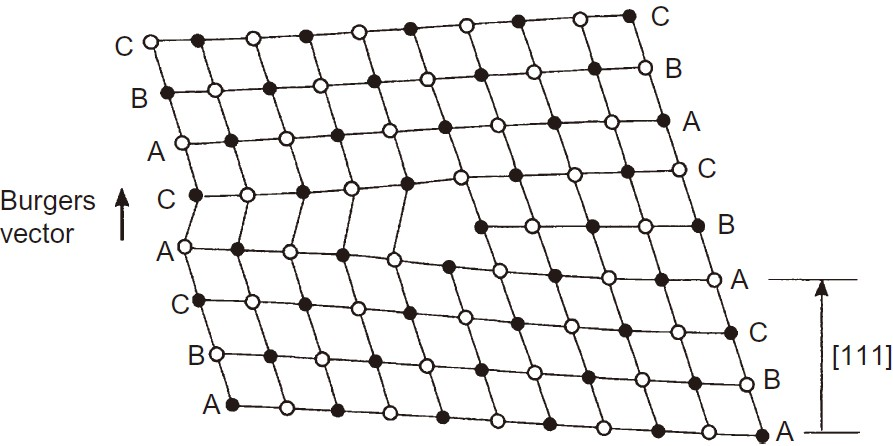
\includegraphics[width=0.5\textwidth]{fig/Formation_of_a_Frank_partial_dislocation.jpg}
                    \caption{密排面的部分原子缺失导致了$\frac{1}{3}\langle111\rangle$偏位错柏式矢量的形成。}
                    \label{Frank_partial_dislocation}
                \end{figure}
                
                面心立方晶体中另一种重要的偏位错为Shockley偏位错\index{Shockley偏位错},柏式矢量为 $\frac{1}{6}\langle 112 \rangle$。
                \autoref{Shockley偏位错模型}中晶体左上角相对其它部分移动了$\frac{1}{6}[\bar{2}11]$,结果
                在晶体左侧$(111)$晶面的堆垛次序发生改变,出现了一片与抽出型层错相同的层错。
                对这篇层错的边界线应用柏式回路方法进行分析,发现它具有的柏式矢量为$\frac{1}{6}[\bar{2}11]$,
                所以这片层错的边界线就是Shockley偏位错。
                \begin{figure}[ht]
                    \centering
                    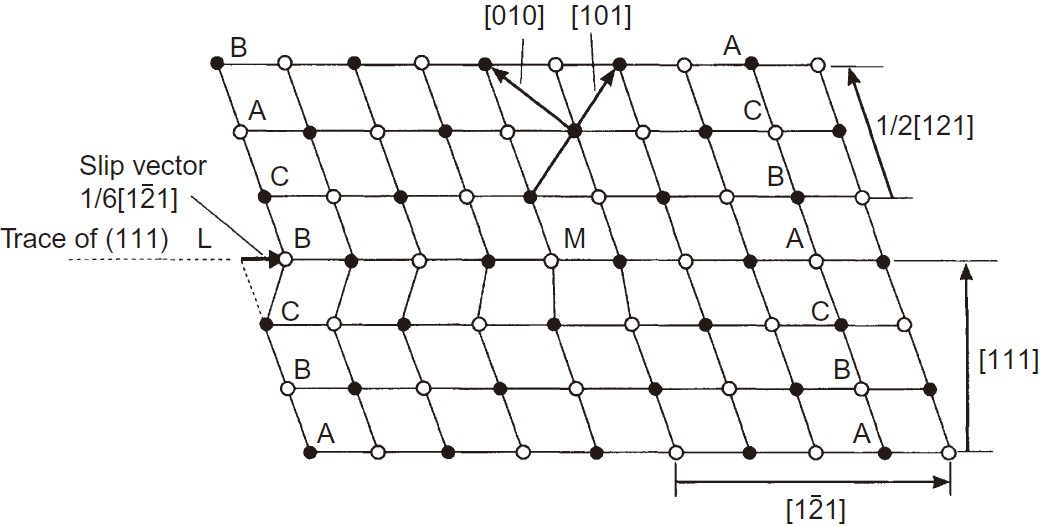
\includegraphics[width=0.5\textwidth]{fig/Formation_of_a_Shockley_partial_dislocation.jpg}
                    \caption{Shockley偏位错模型。}
                    \label{Shockley偏位错模型}
                \end{figure}
                
                \autoref{Shockley偏位错模型}中的位错为纯刃型位错,根据柏式矢量和位错线夹角的关系,也可以
                是螺型或是混合型位错,而且Shockley偏位错可以滑移,滑移面就是${111}$面,然而即使是刃型的
                Shockley偏位错也不能攀移,因为这也会造成严重的错排面。

                关于面心立方的位错总结如\autoref{面心立方的位错类型}
                \begin{table}[ht]
                    \begin{center}
                        \caption{面心立方的位错类型。}
                        \label{面心立方的位错类型}
                        \begin{tabular}{cccc}
                            \toprule
                            名称&全位错&Shockley偏位错&Frank偏位错 \\
                            \midrule
                            柏式矢量& $\frac{1}{2}\langle 110 \rangle$& $\frac{1}{6}\langle 211 \rangle$& $\frac{1}{3}\langle 111 \rangle$ \\
                            位错线&空间曲线&$\left\{ 111\right\}面上的曲线$&任意曲线\\
                            类型&3种&3种&仅有刃型\\
                            运动方式&滑移和攀移&滑移&攀移\\
                            形成方式&切变&$\left\{ 111\right\}$面上的滑移&插入或抽去一层\\
                            \bottomrule
                        \end{tabular}
                    \end{center}
                \end{table}

            \subsection{面心立方的扩展位错}
                面心立方全位错的柏式矢量为$\frac{1}{2}\langle 110\rangle$,可以通过
                位错翻译在$\left\{ 111\right\}$面上分解为两个Shockley偏位错,例如,在
                $(111)$面的$\frac{1}{2}[\bar{1}10]$可按
                \begin{equation}
                    \frac{1}{2}[\bar{1}10]\to\frac{1}{6}[\bar{2}11]+\frac{1}{6}[\bar{1}2\bar{1}]
                \end{equation}
                在分解之后,位错自身的能量减少$\frac{1}{6}$,这在能量上是可行的。而$(111)$面的4个柏式矢量都可以发生分解
                \begin{equation}
                    \begin{aligned}
                    \frac{1}{2}[110]\to\frac{1}{6}[211]+\frac{1}{6}[12\bar{1}]\\
                    \frac{1}{2}[\bar{1}01]\to\frac{1}{6}[\bar{2}11]+\frac{1}{6}[\bar{1}\bar{1}2]\\
                    \frac{1}{2}[0\bar{1}1]\to\frac{1}{6}[1\bar{2}1]+\frac{1}{6}[\bar{1}\bar{1}2]
                    \end{aligned}
                \end{equation}
                如\autoref{111面的全位错分解为Shockley偏位错}所示。
                \begin{figure}[ht]
                    \centering
                    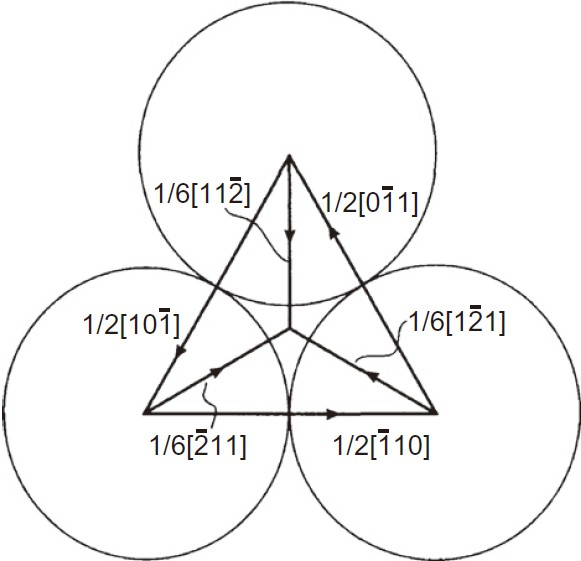
\includegraphics[width=0.5\textwidth]{fig/perfect_burgers_vector_to_shockley_partial_vector.jpg}
                    \caption{${111}$面的全位错分解为Shockley偏位错。}
                    \label{111面的全位错分解为Shockley偏位错}
                \end{figure}

                两个偏位错柏式矢量的夹角小于$\frac{\pi}{2}$可知,它们是互相排斥的;另一方面
                层错的表面张力却要求他们尽量靠近。随着两个片尾错的原理,相互排斥了逐渐降低,直到层错表面张力相等,位错
                之间的距离不再变化,这个平衡距离就是扩展位错的的扩展宽度。如果
                原位错与其柏式矢量的夹角为$\psi$,则两偏位错与柏式矢量的夹角分别为$\psi+\frac{\pi}{6}$
                和$\psi-\frac{\pi}{6}$,两个位错都化成刃型位错和螺型位错的分量,然后利用 \autoref{两个螺型位错之间的作用力}
                和\autoref{两个刃型位错之间的相互作用力},可以得到,片尾错之间的排斥力为
                \begin{equation}
                    F_{12}=\frac{\mu b^2(2-v)}{8\pi d(1-v)}\left[ 1-\frac{2v}{2-v}\cos{2\psi} \right],
                \end{equation}            
                其中$d$为两位错间距,$b$为偏位错强度。平衡时,$F_{12}$等于层错的表面
                张力,而表面张力与层错能$\gamma$像等,所以$F_{12}=\gamma$,代入上式,
                解出扩展宽度为
                \begin{equation}
                    d=\frac{\mu b^2(2-v)}{8\pi \gamma(1-v)}\left[ 1-\frac{2v}{2-v}\cos{2\psi} \right],
                \end{equation}
                由此可见,位错的扩展宽度与层错能成反比。

                扩展位错的运动很简单,实际上就是两个偏位错的运动。但是如果扩展位错是由
                螺型位错分解而来,它还可以进行交滑移。这时扩展位错交滑移分两步:束集(扩展位
                错合并成全位错),交滑移(螺位错变换滑移面的运动),如\autoref{扩展位错的交滑移过程}所示。
                \begin{figure}[ht]
                    \centering
                    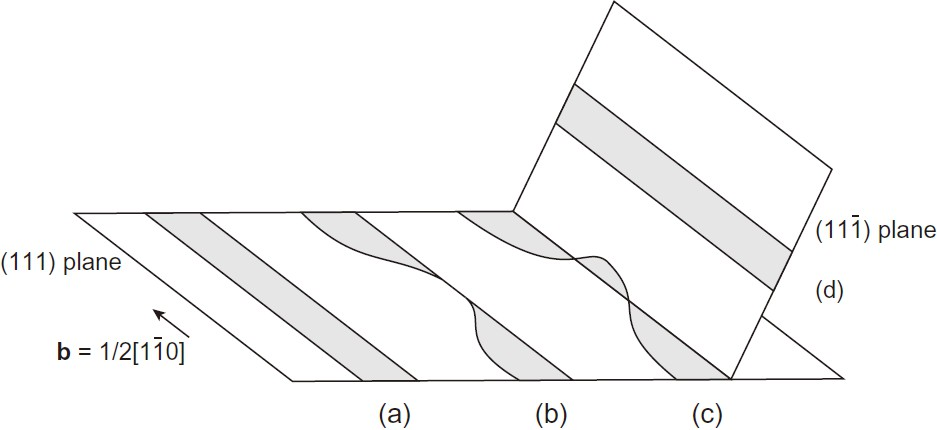
\includegraphics[width=0.7\textwidth]{fig/Four_stages_in_the_cross_slip_of_a_dissociated_dislocation.jpg}
                    \caption{螺位错从$(111)$面转移到$(11\bar{1})$面的四个过程。}
                    \label{扩展位错的交滑移过程}
                \end{figure}
                扩展位错交割时也先束集。所以层错能小,扩展位错宽度大,不易束集,不易运
                动,不易交割。
            \subsection{面角位错}
                
                假设在两个不同的$\left\{ 111\right\}$滑移面上有两个完整位错,如\autoref{压杆位错的形成}所示。
                如果两个位错在滑移过程中相交,形成一个新的位错$\frac{1}{2}[0\bar{1}1]$,由原来的两个柏式矢量相加得到。
                而且是一个刃型位错。这个面上的点阵阻力很大,无法滑移,这和位错也成为面角位错\index{面角位错}。
                \begin{figure}[ht]
                    \centering
                    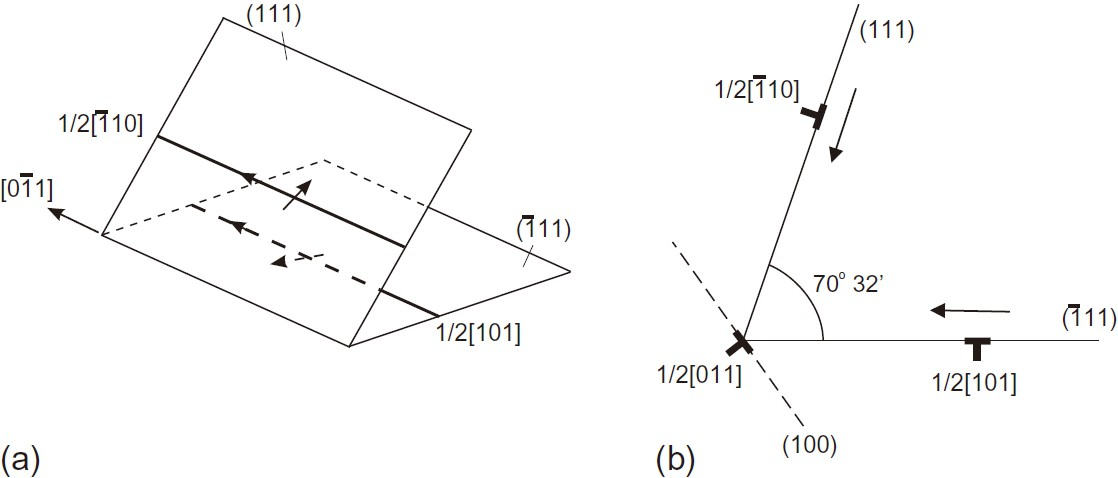
\includegraphics[width=0.7\textwidth]{fig/Formation_of_a_Lomer_sessile_dislocation.jpg}
                    \caption{压杆位错的形成。}
                    \label{压杆位错的形成}
                \end{figure}

                若为两个扩展位错相遇,则领头的两个位错合成新位错,滑移面由于阻力大而不能滑移。
                两个跟着的扩展位错也将受牵制而不动,组态不动,成为其它滑移的障碍物,面角位错也是加工硬化现象的一个重要原因。
	\chapter{晶粒边界}
    多晶体材料中,多个晶粒在凝固时的方向不同,因此在边界处的排列方式需要研究,将两个晶粒之间的边界称为晶界\index{晶界}。
    它是把结构相同但相位不同的两个晶粒分隔开的面状晶格缺陷,是本课程中除了层错以外的另一种面缺陷。

    如果吧晶界看作两个晶粒由于取向差的不同造成了晶界,可以发现,界面在空间的方程有2个自由度,而取向差可以认为是有一个晶粒相对与另一个晶粒进行了旋转,这样,可以说
    旋转轴这条直线的方程中有2个自由度,最后旋转角度为第5个自由度:
    \begin{itemize}
        \item[1] 位相差$\theta$;
        \item[2] 发生位相差$\theta$的转动轴的方向余弦,其中仅有两个是独立的量;
        \item[3]  晶界面法线的方向余弦(其中任意二个),这个方向是用来表示晶界在空间取向的。 
    \end{itemize}
    概括起来,就是产生位相差的转动角$\theta$,表示转动轴上单位矢量$\vec{U}$方位的两个参数以及表示晶界发现单位矢量$n$的两个参数。
    假如直到了这些参变量和晶型,就可以确定晶界的位错模型。
    \section{晶界结构}
        一组平行排列的直的刃型位错的稳定平衡位置是沿$y$轴成了一条直线排列,形成位错墙,而形成这一位错墙的原因是墙的两侧有着较大的取向差。
        \subsection{小角度晶界}
            简单晶界有两种类型:倾斜晶界和扭转晶界。设$U$是发生位相差的相对旋转轴上的单位矢量,$n$是晶界面法线上的单位矢量,则纯粹倾转晶界的条件是    
            \begin{equation}
                U\cdot n=0,
            \end{equation}
            如果晶界面与产生取向差的旋转轴垂直,即$U\parallel n$,就构成了简单的扭转晶界。
            \subsubsection{倾转晶界}
                假设两个简单立方晶体具有相同的$[001]$轴,它们之间的位向差是绕着共同轴相对转动$\theta$角而产生的,两个晶粒的截面是一个对称面,
                都和$(100)$面平行。两个晶体以这种方式连接必然导致连接区域的畸变,而且弹性变形区将扩展到足以松弛晶界的应力集中。除了弹性形变还需要一些竖直
                的原子面终止在晶界上,形成刃型位错,其柏式矢量基本都是$[100]$平移矢量,而柏式矢量$\vec{b}$、位错间距$D$和位相差$\theta$的关系为:
                \begin{equation}
                    \frac{b}{D}=\theta,
                \end{equation}
                当$\theta$小于\ang{15}时,为小角晶界,大于\ang{15}时,为大角晶界。
            \subsubsection{扭转晶界}
        \subsection{大角度晶界}
            对于大角晶界仍然没有得到完美的研究结果,此处主要介绍当前的研究进展。

            过冷液体模型认为大叫晶界是几层原子排雷而成,与过冷液体类似,呈非晶态。但是过冷液体在热力学上不稳定,而晶界存在符合平衡条件。
            另外这一模型认为晶界层上将有两个固液界面,这是不能实现的。

            之后又提出了小岛模型等,都不能解释晶界结构。目前较为有效的模型有重合位置电子模型(CSL),假设一下特殊位向的晶界中,有一些原子同属于两边晶粒的格点,
            并自身形成超格点点阵。模型认为大角晶界由约两原子直径厚的对拍和错排区后才,重合位置点阵和大角晶界的关系:
            \begin{itemize}
                \item[1] 重合关系只出现在某些特定的晶界上,晶界总处于重合点阵的最密排面上,而且能量最低厚度很小,长程应变场可以忽略不计;
                \item[2] 晶界与重合电子的最密排面间有一个小角度时,为了使晶界在重合点阵的最密排面上有最大的面积起见,便会产生阶。阶也不具有长程应变场,但如果在晶界上加一适当的应力,它可能成为位错的增殖源;
                \item[3] 与理想重合位置位向稍有偏离的晶界,可以用一个重合位置晶界同一与它在同一平面上的晶界位错网络叠加在一起来描述。一般这种晶界位错的柏氏矢量较晶格位错的为小,故有次位错之称。
            \end{itemize}

            后来又提出了O点阵的概念,O点阵的结点是指在点上看各自晶格近邻关系是相同的,只差一个转角的点,不一定是原子占据的点。
    \section{晶界能量}
        晶界能量来源于两个晶粒边界上很多原子从晶格的正常位置移动出来,并且在附近晶体中引起畸变。我们定义单位面积所对应的能量增加量为晶界能量\index{晶界能量}。
        \subsection{小角度晶界的能量}
            在晶界的各种性质中,晶界能是很重要的物理量,目前关于小角晶界能的计算有
            很多方法。下面介绍一种简明近似的方法,以对称倾斜晶界为例。单位长度位错的能量为:
            \begin{equation}
                W=\frac{\mu b^{2}}{4 \pi(1-v)} \ln \left(\frac{r_{1}}{r_{0}}\right)+W_{A B},
            \end{equation}
            其中,$W_{AB}$为刃型位错中心能,$r_1$为位错弹性应力场所及的距离,大小为亚晶尺寸,$r_0$为位错核心区。

            在单位长度内的位错数量为$1/D$,$D$为位错间距,
            根据
            \begin{equation}
                \frac{1}{D}=\frac{\theta}{b},
            \end{equation}
            另$b=r_0$,$r_1=D$,位错的能量可以写作
            \begin{equation}
                \begin{split}
                    W&=\frac{\theta}{b}\left[\frac{\mu b^{2}}{4 \pi(1-v)} \ln \left(\frac{1}{\theta}\right)+W_{A B}\right]\\
                    &=\frac{\mu b \theta}{4 \pi(1-v)} \ln \left(\frac{1}{\theta}\right)+\frac{\theta}{b} W_{A B}\\
                    &=E_{0} \theta[A-\ln \theta],
                \end{split}
            \end{equation}
            
        \subsection{大角度晶界的能量}
            由于大角晶界结构未知,可以使用测量的方法,假设三个晶界相较于一个公共的交线,平衡的条件为
            \begin{equation}
                \mathrm{E}_{1} / \sin \psi_{1}= \mathrm{E}_{2} / \sin \psi_{2}=\mathrm{E}_{3} / \sin \psi_{3};
            \end{equation}
            一般测量时习惯将两大角晶界能当作不变的参值,而改变第三晶界的旋转角。
            也可用表面沟槽法,表面张力为
    \section{晶界的运动}
        \subsection{小角晶界的移动}
            晶界的应力感生迁移,晶界受到的力为
            \begin{equation}
                P=\tau\cdot b=\theta\cdot\tau,
            \end{equation}
            晶界的迁移率为$B$,驱动力$F$,则迁移速度为
            \begin{equation}
                v=F\cdot B,
            \end{equation}
            驱动力
            \begin{equation}
                F=\frac{\dif \mu}{\dif x},
            \end{equation}
            也就是反化学位梯度的方向\footnote{扩散中原子的运动的方向为化学位的梯度方向}。
            

\part{性能强化}
	\chapter{晶体的范性变形}
    当金属和合金受力时首先产生弹性变形,以后再开始进入塑性变形(或称范性变形)。塑性变形继续进行直到材料发生
    断裂之前的过程称为流变过程。在流变过程中材料受力与变形的相互对应关系对了解材料的内部特性非常重要,因此
    测量并分析材料的应力应变曲线也是关键的一步。一般材料的应力应变曲线的测定要遵循国标,
    其中关键的控制因素就是应变速率要一定。

    如果定义试样的原始横截面积$A_0$,瞬时横截面积为$A_i$,原始长度为$l_i$,
    断口横截面积为$A_f$,试样所受载荷为$P$,可以得到工程应力应变和真实应力应变。

    假设试样在拉伸过程中体积不发生改变,此时计算出的应力和应变为工程应力\index{工程应力}$\sigma_e$和工程应变\index{工程应变}$\varepsilon_e$有如下定义:
    \begin{align}
        \sigma_{e}&=\frac{P}{A_0},\\
        \varepsilon_{e}&=\frac{\Delta l}{l_0},
    \end{align}
    但是在拉伸过程中,试样会出现颈缩现象,这与假设不符,因此又引入了工程应力\index{真实应力}$\sigma_t$和工程应变\index{真实应变}$\varepsilon_t$:
    \begin{align}
        \sigma_{t}&=\frac{P}{A_i},\\
        \varepsilon_{t}&=\ln\left( \frac{l_0}{l_i} \right).
    \end{align}

    根据两种不同的定义,将实验中得到的拉应力和试样的形变量作出对应的曲线也有两种,
    分别为工程应力应变曲线\index{工程应力应变曲线}和真实应力应变曲线\index{真实应力应变曲线}。

    对于工程应力应变曲线,在开始阶段呈线性变化,金属内部仍为弹性变形。
    。应力达到屈服应力时出现锯齿状平台,而后发现应力虽应变增加而增加阶段,是为加工硬化阶段。
    然而当应力越过最高点后会有一个下降段直到断裂。部分材料在拉伸过程中的屈服平台和
    屈服点都不明显,人为定义永久塑性形变为0.2\%时的应力为屈服点,用$R_{p0.2}$表示。
    工程应力应变曲线虽然不能反映实际的应力应变,但是操作比较简单,因此被广泛使用。

    对于真实应力应变曲线\index{真实应力应变曲线},也分为两段,首先也是线性变化,而后逐渐偏离
    直线过渡到向上弯曲,即弹性变形。在真实应力应变曲线上,没有明显屈服点,但是有两个应力需要注意,
    一是弹性极限$\sigma_{\mathrm{p}}$,即应力小于$\sigma_{\mathrm{p}}$时,只有弹性形变,另一个
    也是人为规定的应力,这里不作介绍。从应力应变曲线上求出曲线包围的面积,也就是变形所作的功,
    这一个值定义为材料的韧性,也是断裂过程所吸收的能量。

    研究发现,试样开始屈服到发生颈缩,阵营里应变满足经验关系
    \begin{equation}
        \sigma=K\varepsilon^n,
    \end{equation}
    $n$为加工硬化指数\index{加工硬化指数},$K$为强度系数,对上式取对数得到
    \begin{equation}
        \ln\sigma=\ln K+n\ln\varepsilon, 
    \end{equation}
    $n$在数值上等于试样的均匀变形量。不同的材料如果根据直线斜率$n$分为
    \begin{itemize}
        \item 理想弹性体,$n=1$,真应力应变曲线的斜率为1;
        \item 理想塑性体,$n=0$,真应力应变曲线为水平直线;
        \item 一般材料,$0<n<1$,曲线斜率在0到1之间。
    \end{itemize}
    \section{单晶体的滑移变形}
        前面已经提到,位错的滑移可以引发材料发生塑性变形,因此材料的塑性变形方
        式包括位错的滑移,孪生;高温状态下还会有晶界滑动方式。
        \subsection{滑移晶体学特征}
            位错滑出晶体后,会在晶体表面造成台阶,早期的研究发现,相同点阵结构的材
            料其相互错动的晶面(也就是位错的滑移面),错动方向称为滑移方向,总是有确定的
            指数,定义一个滑移面和一个滑移方向构成1 个滑移系。

            人们发现滑移面,即能够发生滑移的晶面,往往是原子密排面,这与位错滑移的
            点阵阻力较小有关,在滑移面上按一定晶向进行的滑移方向,是原子的密排方向。
            \autoref{常见的几种点阵类型的滑移系统}总结处常见的几种点阵类型的滑移系统。
            \begin{table}[ht]
            \centering
            \caption{常见的几种点阵类型的滑移系统。}
            \label{常见的几种点阵类型的滑移系统}
            \begin{tabular}{ccccc}
            \toprule
            &滑移面&滑移方向&滑移系个数&条件\\
            \midrule
            FCC&$\left\{ 111\right\}$& $\langle 111 \rangle$ &12& \\
            \multirow{3}*{BCC}&$\left\{ 110\right\}$&\multirow{3}*{$\langle 111 \rangle$}&12&\\
            &$\left\{ 112\right\}$&&12&\\
            &$\left\{ 123\right\}$&&24&\\
            \multirow{2}*{HCP}&$\left\{ 0001\right\}$&$\langle 11\bar{2}0 \rangle$&3&$c/a>1.633$\\
            &$\left\{ 10\bar{1}0\right\}$&$\langle 11\bar{2}0 \rangle$&3&$c/a<1.633$\\
            \bottomrule
            \end{tabular}
            \end{table}
        \subsection{影响滑移系统的因素}
            研究发现,滑移系统不仅与晶体的点阵类型有关,而且还受到其它因素的影响:
            \begin{enumerate}
                \item 温度:当温度升高时,滑移系也增加;
                \item 应变速率:应变速率增大相当于温度降低,滑移系有可能减少;
                \item 合金化元素对不同晶体结构影响不同:
                \begin{enumerate}
                    \item 面心立方加入合金化元素一般对滑移系不产生影响;
                    \item 体心立方加入合金化元素后,对48个滑移系产生选择性;
                    \item 合金化元素对六方结构的影响取决于$c/a$的比值变化。 
                \end{enumerate}
            \end{enumerate}
        \subsection{滑移方式与滑移带}
            实验表明,材料发生范性形变之后,用光学显傲镜观察变形晶体的表面时常常看到一些线状痕迹,如
            如\autoref{单相黄铜中的滑移带}所示。
            这些痕迹是滑移面和晶体外表面的交钱,称为滑移线。如果进一步放大观察,
            可以发现滑移线有精细结构,用电子显微镜观察变形晶体的表面时发现,原来用光学显微镜观察到的
            “滑移线”实际上是由彼此靠近的一组滑移线构成的,称为滑移带。

            在形变过程中,滑移带中,滑移线间没有发生滑动的中间区域叫做滑移层,它们的宽度一般在几十个纳米之间。
            \begin{figure}[ht]
                \centering
                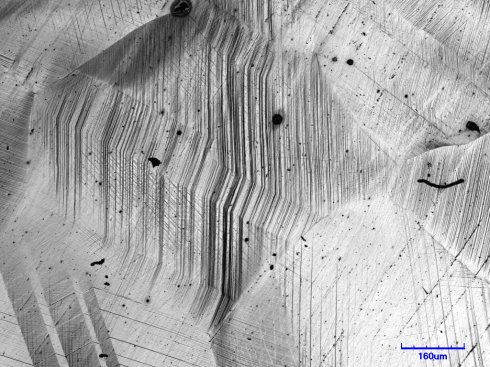
\includegraphics[width=0.5\textwidth]{fig/slip_band_twin_crystal.png}
                \caption{单相黄铜中的滑移带,滑移带在孪晶的位置会发生弯折。图片来源于\href{http://blog.sina.cn/dpool/blog/s/blog_674374ae0101dz8p.html}{quantimet720金相技术}的博客}
                \label{单相黄铜中的滑移带}
            \end{figure}
            
            根据材料中动作的滑移系的状况可以定义:
            \begin{itemize}
                \item 单滑移:只有一个滑移系动作;
                \item 双滑移:两个滑移系同时开动;
                \item 多滑移:多个滑移系同时开动;
                \item 铅笔型滑移:滑移线由具有共同滑移方向的若干滑移面的滑移所组成,(bcc晶体中,多个滑移面向单方向滑移)也称为交叉滑移\footnote{注意不是交滑移,交滑移是指螺位错变换滑移面。}。
            \end{itemize}
    \section{单晶体屈服与晶体的转动及碎化}
        \subsection{临界分切应力定律}
            人们发现,要使单晶体发生滑移,在滑移系上作用的切应力必须达到一个临界值,
            与在该晶面上作用的正应力无关。这个切应力成为临界分切应力。

            当拉伸轴与单晶体的位相关系已知,可以计算作用在滑移系上的分切应力。 
            
            临界分切应力大小与杂质的关系很大也与温度有关。温度升高,临界分切应力下降,
            其下降速率随温度升高而降低,不同滑移系的临界分切应力随温度的升高而趋同。
        \subsection{临界切应力的位错理论}
            晶体收到外应力作用,取向因子最大的滑移系位错开始滑移,其他位错或晶体缺陷要对它的运动产生
            阻碍或交互作用,主要考虑以下几种
            \begin{enumerate}
                \item[1] 位错增殖;
                \item[2] 点阵阻力;
                \item[3] 与其他位错的交互作用:
                \begin{enumerate}
                    \item[1] 弹性应力场的交互作用。为了简便起见,设有二个位错排列在垂直的方向,相距为l。位错要从B、C中间穿过去,就要克服B、C的长程弹性作用力。假设平行于可动位错的那些位错均匀分布,这些位错之间的间距用$l_1$表示,可以推导得出:位错克服的应力为$\tau=\alpha\mu b\sqrt{\rho}$。
                    \item[2] 位错塞积;塞积导致应力集中\footnote{如果塞积群与所求位错之间距离较远,可以视塞积群为一个扩大$N$倍的柏式矢量,其中$N$为塞积群位错数量。}。位错受到的阻力为$\tau_0^2=\alpha\frac{\mu b}{l_2}$
                    \item[3] 位错绕过位错林;与增殖过程相似,在林位错周围形成位错环,然后继续滑移,阻碍切应力为$\tau_0^3=\alpha\frac{\mu b}{l_2}$;
                    \item[4] 以上的三个$\alpha$并非同一常数,仅仅为方便使用同一符号,而且以上的阻力与位错的温度没有关系,
                    \item[5] 切过林位错产生交割,这一部分是短程相互作用,与热激活有关,这是温度升高,屈服强度降低的原因。外力为$\tau$,长程应力为$\tau_0$,外力完成完全切割做功为$W=(\tau-\tau_0)bld$,产生割阶的能量为$\Delta H_0$,热激活提供的能量为$\Delta H=\Delta H_0-(\tau-\tau_0)bld$,当温度高于一定值,形成割阶的能量完全由热激活提供,不需要外力。
                \end{enumerate} 
            \end{enumerate}
            提高屈服强度也就是提高位错运动的长程和短程阻力,主要有以下途径:
            \begin{itemize}
                \item[1] 位错密度上升,比如通过拉拔进行加工硬化,桥梁钢在处理后屈服强度可提升50\%;
                \item[2] 障碍物尺寸增加;
                \item[3] 障碍物间距缩小,也就是增加障碍物密度,比如弥散强化;
                \item[4] 障碍物的稳定性增加。
            \end{itemize}
            影响临界分切应力$\tau_0$的因素
            \begin{itemize}
                \item[1] 高温段不发生变化,温度降低,应力上升,对韧性产生影响;
                \item[2] 合金元素的存在,一般会使临界切应力$\tau_0$增加;
                \item[3] 应变使位错密度增加,进而也会使切应力增加;
            \end{itemize}
        \subsection{拉伸过程中晶体的转动和碎化}
            滑移面与拉伸轴不平行,切变方向沿滑移方向,无法沿拉伸轴方向,因此,试样两端会产生位移。在拉伸实验中,两端被限制,晶面会受到转动力矩的作用,从而发生转动。

            在不能整体发生倾转的时候,表面出现$S$状的滑移线,同号的位错堆积起来,然后产生晶体弯曲,变形过程中晶体的碎化,在取向差小于\ang{15}时\footnote{小角晶界处。},将会出现亚晶。
            产生畸变后,在衍射斑上会出现星芒。
        \subsection{孪生}
            孪生是晶体塑性变形的另一种方式,比如,体心立方的金属的六个偏位错滑移产生孪晶,当晶体的一部分相对另一部分呈镜面对称时,两者互为孪晶。
            
            其与滑移的差异
            \begin{itemize}
                \item[1] 原子到孪生面的移动距离不是常数;
                \item[2] 抛光之后仍然可见;而滑移是表面现象,内部不产生畸变,而孪生不会因为抛光改变晶体排列,仍然可见;
                \item[3] 形状通常为薄透镜状;
                \item[4] 发生速度可以很快;
                \item[5] 一般是滑移受阻时产生的。
            \end{itemize}
        \subsection{总结}
            单晶体塑性变形的三个过程:1.切变,2.转动,3.碎化。
    \section{多晶体范性变形的特点及晶界的作用}
        \subsection{多晶体塑性变形的特点}
            一般情况下,多晶材料屈服应力大于单晶材料,因为晶界会产生强化效应。
            在若干晶系中,选择$\omega$最大的取向最先发生开动,晶粒中发生多滑移,使其发生变形的方向一致。二这需要至少五个滑移系同时运动。
            这也是多晶变形的特点之一:多滑移。

            在晶界附近,为位错滑移受到阻碍,发生位错塞积。

            在变形过程中,会出现择优取向,也就是织构。
        \subsection{多晶体的屈服应力}
            假设在A 晶粒中的某个滑移系处于有利的取向,其取向因子最大,也最先开始滑
            移,滑移后位错遇到晶界,位错塞积,之后在B晶粒的晶界处产生应力集中,当应力集中过大时,
            B中的滑移系达到了临界应力,也会发生滑移,变形也就从$A$传递到了$B$。这是变形的传递过程。

            假设A晶粒中的变形可以表示为
            \begin{equation}
                \gamma=\frac{nb}{L},
            \end{equation}
            其中$L$为A晶粒的滑移方向的长度,
            此时B晶粒没有发生位错滑移,仍然处于弹性变形阶段,所以B中的切应力为
            \begin{equation}
                \gamma^{\prime}=\frac{\tau}{\mu},
            \end{equation}
            两个晶粒的应变应当相同,也就是$\gamma=\gamma^{\prime}$,也就是
            \begin{equation}
                \frac{nb}{L}=\frac{\tau}{\mu},
            \end{equation}
            所以晶界处的位错数为
            \begin{equation}
                n=\frac{\tau L}{\mu b},
            \end{equation}
            位错开始开动时,需要临界分切应力等于该处的集中的应力,因此有
            \begin{equation}
                \tau_c=\frac{n\tau}{\alpha}=\frac{\tau^2L}{\alpha\mu b},
            \end{equation}
            此时外加应力为
            \begin{equation}
                \tau=\sqrt{\frac{\alpha\mu b\tau_c}{L}}=k\cdot L^{-\frac{1}{2}},
            \end{equation}
            屈服应力为
            \begin{equation}
                \tau=\tau_0+k\cdot L^{-\frac{1}{2}},
            \end{equation}
            其中$L$为晶粒尺寸,$\tau_0$为晶格摩擦阻力,$k$为常数,$L$为平均晶粒尺寸。

	\chapter{加工硬化与退火}
    根据霍尔佩奇公式可知,对于多晶材料,当晶粒极端细化时,屈服强度会达到无限大,然而这是不可能的。
    后来根据一些经验,人们认为该公式中应当分段。

    从拉伸曲线上看,当应力大于屈服应力时,应变增加,应力也会增加,这一现象称为加工硬化\index{加工硬化}。
    加工硬化是结构材料的必备性质,使材料的强度得到提高,其益处在于:
    \begin{itemize}
        \item[1] 防止材料被进一步破坏;
        \item[2] 同时保证了材料的均匀变形能力。
    \end{itemize}
    同样也有着一定的坏处
    \begin{itemize}
        \item[1] 加工过程需要退火,变形逐渐困难;
        \item[2] 加工硬化后,材料的韧性降低;
        \item[3] 由于加工硬化能力不足,材料可能会出现缩颈;
    \end{itemize}
    在描述这一性质时有一些参数需要先介绍:
    \begin{itemize}
        \item[1] $n$:加工硬化指数,其数值与最大力对应的型变量相等;
        \item[2] $r$:方形材料的横向变形与纵向变形之比,与内部的织构有关,即滑移面与板面的平行关系;
        \item[3] $\frac{\dif \sigma}{\dif \varepsilon}$:加工硬化率,其与应力应变曲线的交点即为颈缩开始点。
    \end{itemize}
    \section{单晶体加工硬化特征}
        \subsection{面心立方应力应变曲线}
            面心立方晶体的形变效果较好,因此方便研究,也就是不选择体心立方和密排六方的原因。
            实验采用\textbf{单晶面心立方晶体}的加工硬化曲线可以分为三个阶段
            \begin{itemize}
                \item[1] I区:$\dif\tau/\dif\varepsilon$加工硬化率较小,容易滑移,数值大约为$2\times10^{-4}\mu$;
                \item[2] II区:$\dif\tau/\dif\varepsilon$数值基本为常数,大小为$3\times10^{-2}\mu$,称为线性硬化区;
                \item[3] III区:$\dif\tau/\dif\varepsilon$逐渐变小趋于0,称为抛物线硬化区。
            \end{itemize}
            在多晶中难以观察到第一阶段。

            研究发现,有以下因素
            \begin{itemize}
                \item 温度上升使临界分切应力$\tau_c$下降,第一阶段和第二阶段分界点以及第二第三阶段分界点$\gamma_2$和$\gamma_3$显著下降,从而第二第三阶段的切应力都会显著下降;
                \item 层错的影响:拓展位错的宽$d$\footnote{拓展位错宽度增加,层错能下降,交滑移难度增加。}与拓展位错的交滑移,层错能下降,第2第3阶段影响大;
                \item 取向对影响第二阶段分界点和第一部分的斜率;
                \item 合金元素可能是第一阶段增长。
            \end{itemize}

            从滑移线分析,
            \begin{itemize}
                \item [1]第一阶段滑移线较细,在光学显微镜一般观察不到,而且都是相同的指数;
                \item [2]第二阶段的滑移线有交叉,开始双滑移,线长度随型变量的增加而逐步变短;
                \item [3] 第三阶段的滑移带不再连续,位错呈现胞状结构\footnote{与回复阶段有关}。
            \end{itemize}
        \subsection{体心和六方应力应变曲线}
            高纯度的体心立方和六方晶体也是三个阶段,第三阶段与拓展位错交滑移有关,由于体心立方的层错能大,
            因此不容易观察到第三阶段。而观察六方的三阶段更是要求取向合适,因而观察困难。
    \section{加工硬化的位错理论}
        加工硬化的理论主要有两种类型:
        \begin{itemize}
            \item[1] 平行位错硬化理论:与临界分切应力位错理论相似,认为主滑移线的平行位错阻力的长程应力增加;
            \item[2] 交截位错硬化理论:认为林位错对主滑移系产生阻碍,是短程的硬化理论;
        \end{itemize}
        \subsection{第一阶段的位错理论}
        第一阶段位错沿滑移面运动,基本不与其他位错发生交互作用。这一阶段主要是
        位错发生单滑移,
        \begin{equation}
            \tau=\alpha\mu b\rho^{-\frac{1}{2}},
        \end{equation}
        位错源开动,在L-C位错锁\index{L-C位错锁}\footnote{L-C位错锁与双滑移有关,第一阶段为单滑移,L-C位错锁数量不会增加。}附近发生塞积,位错的密度有少量增加,切应力增加。
        假设不动位错的数量为$N''$,单位面积不动位错前塞积的位错数目是有上限的,用$n$表示
        塞积的总位错数为$N''*n$,所以切应力为
        \begin{equation}
            \tau=\alpha\mu nb\sqrt{N''},
        \end{equation}
        此时的变形为
        \begin{equation}
            \gamma=\rho Sb=N''L(nb),
        \end{equation}
        其中$L$为位错长度。
        
        此时的加工硬化率为
        \begin{equation}
            \theta=\frac{\dif\sigma}{\dif \varepsilon}=\alpha\mu\frac{1}{L}\cdot N''
        \end{equation}

        \subsection{加工硬化的第二阶段的理论}
            位错开始发生双滑移和多滑移,位错塞积在L-C位错锁前形成新的位错环。由于仍然是塞积在位错锁,
            所以塞积的上限一定$n$不变,而位错锁前形成新的位错锁,所以$N$增加,也可以说是被激活。
            此时产生的形变的增加为
            \begin{equation}
                \dif \gamma=L(nb)\dif N,
            \end{equation}
            位错的长度为
            \begin{equation}
                L=\frac{\Lambda}{\gamma-\gamma_2},
            \end{equation}
            $\gamma_2$为第二阶段切应变分界点,将$L$带回后积分
            \begin{equation}
                \int(\gamma-\gamma_2)\dif\gamma=\int\Lambda(nb)\dif N,
            \end{equation}
            所以形变变化量为
            \begin{equation}
                \gamma-\gamma_2=\sqrt{2knb\Lambda N},
            \end{equation}
            此时的切应力为
            \begin{equation}
                \tau=\alpha\mu(nb)\sqrt{N},
            \end{equation}
            此时的加工硬化率为:
            \begin{equation}
                \theta_2=\frac{\tau}{\gamma-\gamma_2}=\alpha\mu\sqrt{\frac{nb}{2\Lambda}},
            \end{equation}
            
            这只是理论中的一种,第二阶段的理论仍然有较大争议。
        \subsection{第三阶段的位错理论}
            塞积在不动位错前的螺位错发生交滑移,由于正号和负号的位错相互抵消,使得加工硬化减弱,这一过程与温度的关系很大。
        \subsection{包辛格效应}
            金属在正向加载后然后反向加载,会导致屈服应力降低,在单晶体中不容易观察到,由于这一现象与
            晶界的位错塞积和残余应力有关,因此在多晶体中较为明显。

            比如金属处在高周疲劳情况,屈服应力会不断降低,最后断裂。
    
    \section{多晶体的加工硬化}
        对于多晶体来说,其加工硬化特征也可以分为三个阶段,但是与单晶体的三阶段区别在于一开始就会发生多滑移。

        多晶比单晶多了晶界,而且从滑移一开始就是多滑移。屈服过程是逐步的,没有明确的屈服点。(第一阶段和第二阶段的转折点标志着所有晶粒同时变形)而且晶界是位错运动的重要障碍,所以屈服强度高于单晶的。
        
        二、三阶段位错机制与单晶体相似,所以加大应力后多晶与单晶的加工硬化率逐步接近。
        
    \section{形变金属的加热}
        残余应力有三类,原子层面、单晶层面以及多晶层面。残余应力的大部分能量都来自位错。
        对其加热可以释放应变能,其中会发生三种现象:残余应力消除,发生多边形化,晶粒重新改组,。

        在加热过程中,残余应力消除,发生多边形化是回复的现象,晶粒重新改组为再结晶对应的现象。

        通常情况下,所有境界迁移速度相图,晶粒尺寸均匀。异常情况下,只有少数晶界可以迁移,导致个别晶体形态巨大,
        比如对Al单晶长时间退火,可以形成单晶。

        回复过程中,显微组织组织的变化几乎不可见,再结晶阶段,变形晶粒通过形核长大,逐渐转变为新的无畸变的等轴晶粒,然后等轴晶粒开始长大吸收其它晶粒。

        \subsection{性能变化}
            回复阶段,强度和硬度略有下降,塑性略有提高;再结晶阶段,强度和硬度明显下降,塑性明显提高。
            晶粒长大时,强度硬度继续下降,塑性进一步提高,粗化严重时下降,

            密度会逐渐提高,在再结晶阶段快速提高,电阻在回复阶段可明显下降。


            形变处储存能主要来自弹性应变能、点缺陷和\textbf{位错},在回复阶段开始释放,在再结晶阶段大量释放。
            形变储存能也是回复和再结晶的驱动力。

            回复阶段第一种内应力可以消除,再结晶阶段全部消除。

        \subsection{回复动力学}
            部分材料可以在室温阶段发生回复过程,但是大部分材料都要在较高温度下发生。

            回复过程是动态过程,可以在形变过程中发生,速度较快,时间较短可以发生部分回复,
            加载间隔时间较长可以发生完全回复。

            回复动力学曲线特点
            \begin{itemize}
                \item[1] 没有孕育期;
                \item[2] 开始变化快,逐渐变慢;
                \item[3] 长时间处理后,趋于一个平衡值。
            \end{itemize}

            回复分为根据温度分为低温回复、中温回复和高温回复,以下用$T_m$代表熔点。

            低温恢复发生在0.3$T_m$以下,主要由点缺陷产生
            \begin{itemize}
                \item[1] 空位移到缺陷、位错的地方;
                \item[2]  空位和自间隙原子消失;
                \item[3] 空位发生聚集,
            \end{itemize}
            最后导致缺陷的密度降低,减少弹性畸变能。

            中温回复在$0.3-0.5T_m$发生,异号位错相遇而抵消或者是位错缠结发生重排,因此中温回复的特点为位错密度明显降低。

            高温回复发生在$0.5T_m$以上,位错攀移导致位错垂直排列,产生亚晶界,
            多晶化产生亚晶粒,弹性畸变能降低。
        
            回复的影响因素主要有
            \begin{itemize}
                \item[1] 温度;
                \item[2] 层错能:层错能较低时,攀移位错受阻,难以形成亚晶,或形成不完整亚晶;
                \item[3] 变形量:受到变形越大,
                \item[4] 纯度:纯度越高,再结晶越难发生,回复越易发生。
            \end{itemize}

            主要应用于去应力退火,降低应力,保持加工硬化效果,防止工件变形、开裂,提高耐蚀性。

        \subsection{再结晶}
            形变金属\textbf{加热到一定温度}后,新的无畸变晶粒\textbf{消耗掉冷加工的畸变晶粒}的\textbf{形核与长大过程}。

            新旧晶粒结构相同,因此再结晶不是相变,但是取向完全不同,性能恢复到形变之前。

            发生再结晶的条件是变形量大于临界变形量,这样才能储存足够的应变能。而影响再结晶
            最终的晶粒尺寸与变形量、退火温度以及原始晶粒度有关。

            再结晶温度:经严重冷变形(变形量>70\%)的金属或合
            金,在1h内能够完成再结晶的(再结晶体积分数>95\%)
            最低温度。
            
            在工业中,都是确定变形量和完成再结晶时间固定后才能确定再结晶温度,也就是条件再结晶温度,或称为再结晶停止温度\index{再结晶温度!再结晶停止温度}。

            根据经验公式,纯度越高,越难以发生再结晶,应用时再结晶退火温度比再结晶温度高\SI{100}{\celsius}。

            再结晶的形核过程与相变中的形核过程不同,有两个机制:
            \begin{itemize}
                \item[1] 变形量较大时,在回复过程中由亚晶合并形核,靠亚晶移动形核;
                \item[2] 变形量较小时,大角晶界凸出形核,完全靠晶界迁移,晶核伸向畸变能较高的区域。
            \end{itemize}

            再结晶过程存在孕育期,温度越高,变形量越大孕育期越短;在体
            积分数为0.5时速率最大,然后减慢。

            再结晶温度的影响因素有:
            \begin{itemize}
                \item[1] 变形量越大,驱动力越大,再结晶温度越低;
                \item[2] 纯度越高,再结晶温度越低;
                \item[3] 加热速度太低或太高,条件再结晶温度提高。
            \end{itemize}
            
            对再结晶的影响因素有
            \begin{itemize}
                \item[1] 退火温度。温度越高,再结晶速度越大;
                \item[2] 变形量越大,再结晶温度越低;随变形量增大,再结晶温度趋于稳定;变形量低于一定值,再结晶不能进行;
                \item[3] 原始晶粒尺寸。晶粒越小,驱动力越大;晶界越多,有利于形核。
                \item[4] 微量溶质元素阻碍位错和晶界的运动,不利于再结晶;
                \item[5] 分散第二相,间距和直径都较大时,提高畸变能,并可作为形核核心,促进再结晶;直径和间距很小时,提高畸变能,但阻碍晶界迁移,阻碍再结晶。
            \end{itemize}

            再结晶应用于恢复变形能力、改善显微组织、消除各向异性以及提高组织稳定性。
        \subsection{晶粒长大}
            \subsubsection{正常长大}
            晶粒长大的驱动力为界面能变化,长大方式有两种,分别为
            \begin{itemize}
                \item[1] 正常长大:再结晶后的晶粒均匀连续的长大,驱动力为界面能差,曲率半径越小,驱动力越大,长大方向指向曲率中心;
                \item[2] 异常长大,也称为二次再结晶。
            \end{itemize}

            晶粒正常长大方向是指向曲率的中心,曲率半径越小,驱动力越大,再结晶晶核的长大方向相反。

            晶粒稳定条件是晶界夹角为\ang{120},边界趋于平直,二维坐标的晶粒边数趋于6。

            影响因素有
            \begin{itemize}
                \item[1] 温度:温度越高,晶界易迁移,晶粒易粗化;
                \item[2] 分散相粒子:阻碍晶界迁移,降低晶粒长大速率;
                \item[3] 杂志和合金元素:气团钉扎晶界,不利于晶界移动;
                \item[4] 晶粒的取向差:小角度晶界能小于大角度晶界,前者的移动速率低于后者。
            \end{itemize}

            \subsubsection{晶粒异常长大}
                异常长大是指:少数再结晶晶粒的急剧长大现象。正常的晶粒长大过程被第二相或织构限制。
                驱动力主要是界面能的变化。

                有三种机制:1. 钉扎晶界的第二相溶于基体;2.再结晶织构中位向一致晶粒的合并;
                3. 大晶粒吞并小晶粒。

                对组织和性能的影响是
                \begin{itemize}
                    \item[1] 织构明显,出现各向异性,磁导率强化;
                    \item[2] 晶粒大小不均匀,整个材料的性能不均匀;
                    \item[3] 晶粒粗大,降低了材料的强度和塑性,提高了表面的粗糙度。 
                \end{itemize}

                在金属的轧制过程中,远高于再结晶温度的轧制以及远低于再结晶温度不会产生混晶\footnote{个别晶粒的大小远大于周围晶粒的尺寸。},
                否则会对材料的韧性产生较大危害,尤其在断裂问题中,一个较大晶粒非常容易传导裂纹。

            \subsubsection{再结晶退火的组织}
                首先要参考再结晶图了解退火温度、变形量与晶粒大小的关系图,可能会产生再结晶织构,也就是退火过程中
                形成的新织构;也有可能形成退火孪晶,在面心立方中常见,由于晶界迁移出现层错引起的。

            \subsubsection{动态回复与动态再结晶}
                动态回复是指在塑性形变中发生的回复,拉伸曲线会波动向上;动态再结晶是指在变形过程中发生
                动态再结晶,拉伸曲线在某一值附近波动。

                组织有两个特点:
                \begin{itemize}
                    \item 反复形核,有限长大,最后的晶粒非常细小;
                    \item 包含亚晶粒,位错密度较高,强度和硬度都很高。 
                \end{itemize}

                在生产中采用低的变形终止温度、较大的最终变形量(平均一道次变形量一般要大于70\%),快的冷却速度可获得细小晶粒。
	\chapter{合金强化}
    决定材料强度的关键因素是原子之间的结合力以及位错。原子的结合力与材料的原子有关,这非常难控制,
    但是位错是人类可以控制的重要因素,因此位错是近代金属领域的最大成果。

    \section{强化金属的途径}
        根据位错运动出发,强化的方式主要有两种。
        \subsection{金属的极限强度}
            金属的极限强度约为\SI{6000}{\MPa},然而实际的材料仅仅为极限的$\frac{1}{10}$,
            想要达到这样的强度就必须实现理想晶体,使晶体满足刚性滑移假设。在实际上通常是把位错
            滑移出晶体,但是一旦晶体中出现位错,性能就急剧下降。
        \subsection{人为增加位错的阻力}
            提升晶格阻力和源动作应力是提升强度的重要方法:通过对金属中各种微结构与位错的相互作用提升强度的方法主要有四种
            \begin{enumerate}
                \item[1] 点缺陷:固溶强化;
                \item[2] 线缺陷:加工硬化,写出切应力公式$\gamma=\rho sb$;
                \item[3] 面缺陷:晶粒细化强化,写出霍尔佩奇公式$\sigma_s=\sigma_0+k\cdot d^{-1/2}$;
                \item[4] 体缺陷:分散强化。
            \end{enumerate}
            在工业中,都是使用综合强化。比如同一个奥氏体中的马氏体片条组,可以视为将奥氏体细化实现强化。
    \section{人为强化机制}
        \subsection{固溶强化}
            溶质原子与气团的相互作用有两种,直接作用和间接作用。

            基本规律是
            \begin{itemize}
                \item 固溶体强度大于纯金属,细固溶体的强度与间隙原子的浓度成线性关系,间隙原子半径越小,强化效果越大;
                \item 溶解度小的元素强化作用较大;
                \item 稀固溶体的强化作用可以叠加;
                \item 间隙原子作用大于置换原子;
                \item 相同的电子浓度,强化效果接近;
                \item 模量相应,加入物质的模量越大,强化效果越大。
            \end{itemize}
        \subsection{固溶强化机制}
            \begin{enumerate}
                \item 弹性相互作用:气团,
                \begin{enumerate}
                    \item 是明显屈服点产生的原因,对位错的启动有作用;
                    \item 溶质原子是间隙原子可以使间隙现象更为明显,在体心立方中比面心立方中更明显;
                    \item 对温度敏感,温度升高,扩散加快;
                    \item 只要有少量溶质就可以起作用。
                \end{enumerate}
                \item 溶质原子分布的摩擦阻力;
                \item 电学交互作用:较弱,位错两侧的溶质原子的库仑力产生拉应力或压应力;
                \item 化学交互作用:较弱;
                \item 有序化:主要在有序化的材料中才会出现,分为长程序和短程序,在有序晶体内产生反向畴界。
            \end{enumerate}
            其中第一点、第四点第五点对位错启动有作用,2、3、5总是对位错运动有作用。
            温度升高,第一类作用下降。
        \subsection{屈服现象与应变时效}
            有两种屈服现象,分为有明显屈服平台和无平台(均匀屈服)两种。
            
            第一种的产生原因是科垂耳气团,在超过上屈服点后应力下降,发生动态再结晶,
            这一阶段称为屈服齿,也叫做吕德斯应变,是形变传播过程中的必然现象。

            均匀屈服没有屈服平台,而是呈凹陷区域。在$\alpha$\ce{Fe}经过除\ce{H}处理后,
            可以发现。一般认为是可动位错的密度的提高,导致屈服凹陷的出现
            \begin{align}
                \gamma=\rho sb,\\
                \varepsilon=\phi\rho sb\\
                \dot{\varepsilon}=\phi\rho\dot{s}b.
            \end{align}
            拉伸时,速度一定,所以只能是位错速度下降,出现凹陷。
        \subsection{分散强化}
            如果材料中出现第二相,形成两相合金。在这两种相之间的界面上的原子排列不再具有晶格完整性。在金属等塑性材料中,这些相界面会阻碍位错的滑移,从而使材料得到强化。这就是分散强化的由来。
            分成弥散强化、时效(沉淀)强化两类。

            当位错经过第二相时,会出现绕过机制,形成位错环。或是根据切过机制,位错切过第二相。
        
    \section{补充}
        \begin{enumerate}
            \item 兰脆现象:当钢铁加热到\SIrange{200}{300}{\degree},钢铁的脆性增加,表面变成兰色,原因是钢铁的动态应变时效。
            \item 预应变:提前拉伸钢铁,使其脱开溶质原子的束缚。
        \end{enumerate}
	\chapter{金属的断裂}
    材料在实际的使用过程中,存在一系列的构件失效的现象,其中最为重要的一种就是断裂。
    断裂过程往往突然发生,这会对使用造成巨大的危害,而且无法预期。在这里关注断裂的物理本质。
    对化学问题不做研究。

    断裂在金属材料中被认为是金属材料在变形超过其塑性极限,原子间结合力被破坏,
    结构完全分开。
    断裂的核心问题是研究断裂从何处出现和裂纹如何发展。
    \section{断裂的基本类型}
        根据断裂前金属是否有明显的塑性变形可以分为脆性断裂和韧性断裂,
        一般认为如果变形量$\varepsilon<5\%$就是脆性断裂。

        对于断口的分类有很多种:
        \begin{itemize}
            \item 按照断裂面相对作用力的取向关系可以分为正断和剪断;
            \item 从微观上裂纹的走向可以分为穿晶断裂和沿晶断裂(冰糖断口);
            \item 从晶体学的特征上可以分为切变断裂和解理断裂;
            \item 断口形貌上还分为纤维状断口、结晶状断裂、疲劳断裂和应力腐蚀断口。
        \end{itemize}

        \subsection{解理断裂}
            解理断裂是指当应力达到某一临界值时沿一特定结晶学方向发生的突然断裂\footnote{考试题:三条重点。},
            宏观特征为断口平滑光亮、一般在体心、六方中易于出现。 温度越低、应变速度越大易于出现。
            电子显微镜下的形貌为河流状花样。解理面一般是原子间距最大的晶面,因为此处原子结合键最弱。

        \subsection{韧性断裂}
            经过明显的变形后发生的断裂称为韧性断裂。拉伸时以颈缩为先导,当应变硬化产生的强度增加不足以补偿截面积的减少时,
            产生应力集中变形,出现“细颈”。

            细颈中心承受三向拉应力, 显微空洞首先在此形成, 随后长大聚合成 裂纹, 最终在细颈边缘处,沿与拉伸轴\ang{45}
            方向被剪断,形成“杯锥”断口,在微观形态下,由于夹杂物的存在产生空洞,在拉伸
            过程中产生韧窝。

            韧性断裂的特点:
            \begin{itemize}
                \item 断裂前发生较大塑性变形,吸收大量的能量;
                \item 裂纹产生然后扩展最后聚合;
                \item 裂纹扩展临界应力大于裂纹形核应力,导致裂纹缓慢增加。
            \end{itemize}
    \section{脆性断裂}
        \subsection{理论断裂强度}
            完整晶体在正应力作用下沿某一晶面拉断的强度。两相邻原子面在拉力作用下,克服原子间键合力
            作用,是原子面分开的应力。

            根据原子间作用模型,原子间作用力与位移间的关系满足
            \begin{equation}
                \sigma=\sigma_{m}\sin\left( \frac{2\pi x}{\lambda} \right)
            \end{equation}
            将原子拉开所需的最大应力,即断裂理论强度。
            将两个原子面拉开所做的功为
            \begin{equation}
                \int_{0}^{\frac{\lambda}{2}}\sigma_m\sin\left( \frac{2\pi x}{\lambda} \right)\dif x=\frac{\lambda\sigma_m}{\pi},
            \end{equation}
            断裂后产生两个断裂面,表面能为$2\gamma$,
            外力抵抗原子间结合力所作的功为产生断裂新面的表面能
            \begin{equation}
                \frac{\lambda\sigma_m}{\pi}=2\gamma,
            \end{equation}
            与虎克定律联立解得
            \begin{equation}
                \sigma_m=\left( \frac{\gamma E}{a} \right)^{1/2},
            \end{equation}
            对于一般金属,计算得到的理论断裂强度为\SI{10000}{\MPa},这与实际仅为\SIrange{200}{500}{\MPa}
            的断裂强度不符,因此完整晶体模型在这里仍然是不适用的。
        \subsection{Griffith脆断理论}
            Griffith认为材料在断裂之前已经存在微裂纹,从裂纹尖端引起应力集中,在外加应力小于理论断裂强度
            时裂纹扩展,实际裂纹强度将大大降低。

            理论认为,弹性能减少不仅仅用于材料变形,裂纹长度的增加也消耗了一部分弹性能。根据
            这一理论计算得到的最大断裂强度为
            \begin{equation}
                \sigma_c=\left( \frac{2E\gamma}{\pi c} \right)^{\frac{1}{2}},
            \end{equation}
            其中$c$为晶体中存在的裂纹长度的一半。相当于裂纹两端引起的应力集中把外力
            放大了$\left( \frac{c}{a} \right)^{1/2}$倍,使局部达到了理论断裂强度。
        
            这个理论虽然解释了理论断裂强度与实际的差别,但是其中还是省略一部分,
            比如忽略了脆性断裂之前的塑性形变,因此Orowan对该理论提出了修正公式,
            考虑了塑性变形能
            \begin{equation}
                \sigma_c=\left[ \frac{2E(\gamma+P)}{\pi c} \right]^{\frac{1}{2}},P\gg\gamma,
            \end{equation}
            其中$p$为断口表面的塑性应变能。
        \subsection{裂纹形核}
            运动的位错遇到了某种障碍, 就产生了应力集中,应力大到可以破坏原子间的键合力时,裂纹开始形核,裂纹长大导致断裂。
            
            形核机制有几种:
            \begin{itemize}
                \item[1] 位错塞积,在相界处发生应力集中;
                \item[2] 位错反应,在两相交的滑移面上,由于位错反应发生了同号位错的聚合便产生了微裂纹;
                            比如在体心立方的$(101)$面上发生如下位错反应
                            \begin{equation}
                                \frac{a}{2}[\bar{1}\bar{1}1]+\frac{a}{2}[111]=a[001],
                            \end{equation} 
                            生成的新位错为不滑动刃型位错,其柏氏矢量与$(001)$解理面垂直,形成解理裂纹;
                \item[3] 位错墙侧移理论:热型位错垂直排列,形成位错墙,在滑移面发生弯折,在外力下,位错墙侧移,在滑移面上生产裂纹;
                \item[4] 位错销毁理论:异号刃型位错相对运动,彼此合并形成空隙,以此产生裂纹。
            \end{itemize}
        \subsection{裂纹传播}
            以塞积位错造成裂纹形核为例,产生新的表面和位错的塞积能需要消耗能量,而外力做功和弹性能释放为此提供能量。

            假设形成裂纹时的应力就是屈服应力 滑移带的长度等于晶粒直径$d$,断裂强度
            \begin{equation}
                \sigma_c=\frac{2\mu\gamma}{k} d^{-\frac{1}{2}},
            \end{equation}
            说明晶粒越细,传播阻力越大。由于晶粒取向不同,穿过晶界导致传播转向。这也是提高韧性的方法。
            而且晶粒尺寸越小,试样内存在着道道临界尺寸的裂纹的几率越小,当晶粒尺寸为\SI{1}{\micro\m}时
            断裂强度就可以接近理论断裂强度。
    \section{金属断裂方式的转变}
        \subsection{影响断裂类型的因素}
            在一定条件下,材料可以从韧性断裂转变为脆性断裂。而影响转变的因素有
            有变形温度、变形速率、应力状态和组织结构。

            这里主要关注温度的影响,定义材料的韧脆转变温度为从韧性断裂到脆性断裂的转变温度称为脆性
            转变温度$T_c$。
            
            温度对于断裂应力$\sigma_f$的影响不大,然而温度升高会使材料的屈服强度降低,因此
            温度高于$T_c$,材料的断裂应力$\sigma_f$大于屈服应力$\sigma_s$,因此发生塑性断裂;温度低于$T_c$时
            则发生脆性断裂。
        
            
\part{固溶体、扩散与相变}
	\chapter{固溶体}
    \section{固溶体}
        根据相的结构和形成条件,可以分成三种,固溶体、有序固溶体和金属
        间化合物;很具合金相在相图中的位置,可以将合金相分为纯金属、固溶体
        和金属间化合物。

        本章关注的重点是固溶体,固溶体是指不同元素的原子能够以变动的比例去占据晶体结构
        的位置(点阵)。即固溶体可以在一定的成分范围内存在,性能随成分变化而连续变化。
        固溶体溶解度的极限也称为固溶度。

        不同金属和化合物的固溶度差别很大,可以从几乎不溶解到完全互溶。固溶体
        可以无序,即组元在点阵中随机分布;也可以有序,即异类原子有规则的排列。有序可以是短程的,
        也可以是长程的。

        \subsection{固溶体及其类型}
            有些组元合金化后能形成一系列的固溶体:
            \begin{enumerate}
                \item 一次固溶体\index{一次固溶体}:在含有金属组元的二元相图中,靠近金属组元的一端,一般总会有溶解度不同的固溶体,其晶体结构与溶剂金属相同;
                \item 二次固溶体\index{二次固溶体}:在相图的中间位置,晶体结构不一定与溶剂相同,又叫中间相,即以化合物为基的固溶体。其中为长程序的中间相,称为金属间化合物。
            \end{enumerate}

            根据溶质原子在晶体点阵的位置,可将固溶体分为三类:
            \begin{enumerate}
                \item 置换型:原子大小相近;
                \item 间隙型:原子尺寸差别较大;
                \item 缺位型:格点上某一类原子出现空缺。
            \end{enumerate}
        \subsection{影响固溶度的因素}
            影响固溶度的因素主要有三种,分别是尺寸因素、电子浓度因素和
            化学亲和力因素。
            \subsubsection{尺寸因素}
                若形成合金的组元的原子尺寸差超过14-15\%时,尺寸因素将会产生较大影响,
                使固溶度降低;容尺寸差小于15\%,尺寸因素成为次要的影响因素,固溶度由其他影响因素确定。
                这也就是Hume-Rothery规律\index{Hume-Rothery规律}。

                原子大小一般在\si{\angstrom},不同情况下,测得的原子大小不同,比如
                $\alpha-$\ce{Fe}和$\gamma-$\ce{Fe},原子的配位数分别为8和12,配位数越小,
                原子尺寸越小,所以$\alpha-$\ce{Fe}原子小于$\gamma-$\ce{Fe}。

                当异类原子形成固溶体时,符合Vegard定律,也就是粒子晶体电子常数$a$与固溶体成分$x$
                有线性关系:
                \begin{equation}
                    a=a_1+(a_2-a_1)x=a_1(1-x)+a_2x,
                \end{equation}
                其中$a_1$是溶剂的点阵常数,$a_2$是溶质的点阵常数。然而金属固溶体都或多或少偏离
                离子晶体,故也偏离Vegard定律,有的出现正偏差,有的出现负偏差。
            \subsubsection{电子浓度因素}
                电子浓度\index{电子浓度}是指价电子数和原子数的比值,记做$e/a$
                如果溶质原子的百分数为$x$,原子价为$v$,而溶剂的原子价为$V$,则合金的电子浓度为
                \begin{equation}
                    \frac{e}{a}=\frac{v x+(100-x) V}{100}.
                \end{equation}

                电子浓度对于原子是不确定的,由于原子“价”是不固定的。比如,一般认为
                \ce{Zn}是$+2$价,但已经证明,$+1$价电子完全贡献出来,第二个电子并不完全贡献
                出来,而仍有一定几率绕\ce{Zn}原子核转动,所以\ce{Zn}的价不是$+2$。
            \subsubsection{化学亲和力因素}
                原子的第一电离能\index{第一电离能}$E_I$是气态原子失去一个电子成为气态的
                一价正离子所需的能量,
                \begin{equation}
                    E_I=E(M^+)-E(M),
                \end{equation}
                其中$M$为原子。

                原子的电子亲合能$Y$是原子获得一个电子成为一价负离子
                时所放出的能量,即
                \begin{equation}
                    -Y=E_(M^-)-E(M),
                \end{equation}
                电子亲合能和第一电离能都可以通过实验测定。

                而A、B两原子形成$\mathrm{A}^{-}\mathrm{B}^{+}$必须满足
                \begin{equation}
                    E_{IA}+Y_{A}>E_{IB}+Y_{B},
                \end{equation}
                以$E_I+Y$表示\textbf{化学亲合力}\index{化学亲和力},通常称之为\text{负电性}\index{负电性}。
                它表示组元吸引电子的能力。负电性越大的组元,吸引电子的
                能力也越强。形成离子化合物时,负电性大的元素成为负离子,负电性小的成为正离子。

                实际只需负电性的相对大小,人为规定氟的负电性为4.0。负电性有周期性。但贵金属\ce{Cu}、\ce{Ag}、
                \ce{Au}是例外。负电性概念比较适用于金属间化合物。
        \subsection{固溶体自由能的统计理论}
            根据共晶型相图\autoref{CuAg相图},BC和GH分别代表组元B在A中和A在B中的溶解度曲线,实际上就是在不同温度下的浓度曲线$c(T)$
            \begin{figure}[ht]
                \centering
                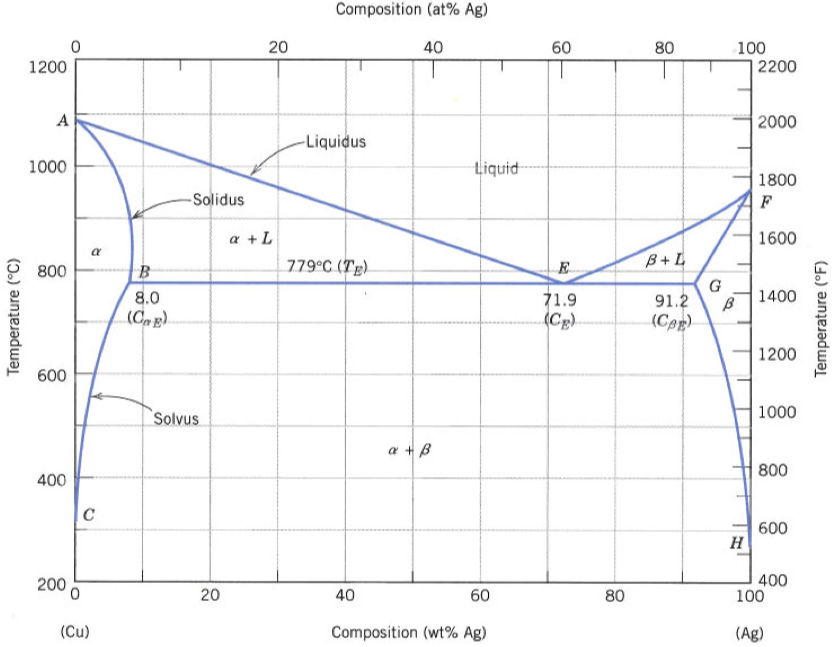
\includegraphics[width=0.7\textwidth]{fig/Cu_Ag_Phase_Diagram.png}
                \caption{\ce{Cu}和\ce{Ag}的相图,图片来源:\href{http://resource.npl.co.uk/mtdata/phdiagrams/agcu.htm}{National Physical Laboratory}。}
                \label{CuAg相图}
            \end{figure}

            要求解浓度$c(T)$,及必须先求解体系自由能$F(c,T)$,再利用相平衡求出$c(T)$,即
            固溶度方程。

            在求解自由能时需要用到准化学近似\index{准化学近似},假定固态原子之间存在化学键,因而晶体的
            内能可以按拆散或形成的键数用统计方法加以计算。假设A、B组元形成置换固溶体,原子浓度
            分别为$(1-c)$和$c$,假设原子总数为$N$,则有
            \begin{align}
                N_A&=N(1-c)=N-n,\\
                N_B&=Nc=n.
            \end{align}
            自由能为
            \begin{equation}
                F=E-TS,
            \end{equation}
            因此,应当先表示体系的内能和熵。假设固溶体在\SI{0}{\K}的内能为$E_0$,比热为
            $C_p$,则在$T$时的内能和熵为
            \begin{align}
                E&=E_0+\int_{0}^{T}C_p\dif T,\\
                S&=\Delta S_{\mathrm{m}}+\int_{0}^{T}\frac{C_p}{T}\dif T.
            \end{align}
            式中$\Delta S_{\mathrm{m}}$为混合熵:
            \begin{equation}
                \Delta S_{\mathrm{m}}=k\left( \ln\omega_{AB}+\ln\omega_{A}+\ln\omega_B \right)\label{固溶体系的混合熵}.
            \end{equation}
            在热力学上,单质的组态熵为零,因此$\omega_A=\omega_B=1$,而固溶体的组态熵为
            \begin{equation}
                \omega_{AB}=\frac{N!}{N_A!N_B!}=\frac{N!}{n!(N-n)!},
            \end{equation}
            代入\autoref{固溶体系的混合熵}可得
            \begin{equation}
                \Delta S_{\mathrm{m}}=k\ln\frac{N!}{n!(N-n)!},
            \end{equation}
            利用Stirling近似,可得
            \begin{equation}
                \Delta S_{\mathrm{m}}=k[N\ln N-n \ln n-(N-n) \ln (N-n)],
            \end{equation}
            因为$c=n/N$,$1-c=(N-n)/N$,所以变成
            \begin{equation}
                \Delta S_{\mathrm{m}}=-N k[c \ln c+(1-c) \ln (1-c)],
            \end{equation}
            由于浓度均小于1,所以$\Delta S_{\mathrm{m}}>0$。

            对于内能的求解则从结合能出发,假设A、B形成固溶体是,晶体中无缺陷,原子紊乱分布,
            则晶体中存在三种键AA、BB和AB的个数分别为
            \begin{align}
                N_{AA}&=\frac{1}{2}N(1-c)\cdot(1-c)\cdot Z,\\
                N_{B B}&=\frac{1}{2} N c \cdot c \cdot Z,\\
                N_{A B}&=N c \cdot(1-c) \cdot Z.
            \end{align}
            原子间作用能用$V$表示,内能$E_0$等于合金中所有最近邻原子间作用能之和
            \begin{equation}
                \begin{aligned}
                    E_{0}&=V_{A A} N_{A A}+V_{B B} N_{B B}+V_{A B} N_{A B}\\
                    &=\frac{1}{2} N Z\left[(1-c)^{2} \cdot V_{A A}+c^{2} \cdot V_{B B}+2 c(1-c) \cdot V_{A B}\right]\\
                    &=\frac{1}{2} N Z\left[c V_{B B}+(1-c) V_{A A}+c(1-c)\left(2 V_{A B}-V_{A A}-V_{B B}\right)\right].
                \end{aligned}
            \end{equation}
            前两项为纯A和纯B的内能,第三项为固溶后内能的改变量$\Delta E$。
            固溶体的形成能为
            \begin{equation}
                \Delta E=NZc(1-c)V=N_{AB}V,
            \end{equation}
            其中$V=V_{AB}-\frac{1}{2}(V_{AA}+V_{BB})$为形成一个AB键时内能的改变量。
            
            不考虑随温度带来热容变化,计算得到的自由能为
            \begin{equation}
                \begin{aligned}
                    F&=E-TS\\
                    &=E_0+\int_{0}^{T} C_{\mathrm{p}} \mathrm{d} T-T\left(\Delta S_{\mathrm{m}}+\int_{0}^{T} \frac{C_{\mathrm{p}}}{T} \mathrm{d} T\right)\\
                    &=K(c, T)+\frac{1}{2} N Z\left[c V_{\mathrm{BB}}+(1-c) V_{\mathrm{AA}}\right]+N Z c(1-c) V\\
                    &+N k T[c \ln c+(1-c) \ln (1-c)].
                \end{aligned}\label{固溶体自由能的表达式}
            \end{equation}
            影响自由能曲线的有两部分$V$和$T\Delta S_m$,因此按照$V=0$、$V<0$和$V>0$可以分为三种情况:
            \begin{enumerate}
                \item[1] $V=0$,即形成固溶体时能量不变,固溶体是理想固溶体,$E_0$为浓度的线性方程,自由能有极小值,不论合金成分如何都会形成单相固溶体;
                \item[2] $V<0$,虽然$E_0$不再是直线,但是也形成单相固溶体;
                \item[3] $V>0$,自由能曲线存在两个拐点\footnote{拐点为二阶导数为零的点。},也就是在这两个拐点之间,体系分解为两相混合物。
            \end{enumerate}

            在计算$E_0$时作出了两个主要的假定:
            \begin{enumerate}
                \item[1] 原子随机分布假定:
                \begin{enumerate}
                    \item 然而只有形成固溶体的内能不变,也就是$V=0$时,内能分布才和原子分布无关,原子才能随机分布;
                    \item 当$V<0$时,形成AB键使内能下降,合金倾向与形成更多的AB键,也就是异类原子相互吸引,此时公式中的$N_{AB}$偏小,但是对内能和熵的影响可以相互补充,对结果影响不大;
                    \item 同理,$V>0$时,对自由能和熵的影响也是相互补偿的,对结果影响不大;
                \end{enumerate} 
                \item[2] 最近邻原子键能的假定:计算$E_0$是,认为它等于合金中所有最近邻原子间作用能之和,但是
                \begin{enumerate}
                    \item 侧重考虑化学亲和力因素,忽略了键所处的环境;
                    \item 当电子浓度因素起主要作用时,价电子属于整个晶体,并不构成定向键;
                    \item 当尺寸因素起主要作用时,畸变能牵涉到若干原子间距,这与研究的体系相关。
                \end{enumerate} 
            \end{enumerate}
        \subsection{固溶度方程}
            假设各个原子之间的结合能相等,各组分的热容也相等,在$N=N_0$也就是\SI{1}{\mol}分子
            的情况下,\autoref{固溶体自由能的表达式}可以写作
            \begin{equation}
                F=K(T)+\frac{1}{2}N_{0} Z V_{0}+N_{0} Z V c(1-c)+N_{0} k T[c \ln c+(1-c) \ln (1-c)].
            \end{equation}
            平衡条件为
            \begin{equation}
                \frac{\dif F}{\dif c}=0,
            \end{equation}
            因此
            \begin{equation}
                \frac{\dif F}{\dif c}=N_{0} Z V(1-2 c)+R T[\ln c-\ln (1-c)]=0.
            \end{equation}
            解得
            \begin{equation}
                \frac{c}{1-c}=\exp \left[-\frac{\mathrm{N}_{0} Z V(1-2 c)}{R T}\right],
            \end{equation}
            这就是固溶度方程\index{固溶度方程}。

            当固溶度浓度很小时,$1-c\simeq 1$,$1-2c\simeq 1$,此时固溶度方程为
            \begin{equation}
                c=\exp \left(-\frac{N_{0} Z V}{R T}\right)\label{低浓度固溶度方程},
            \end{equation}
            所以在固溶度不大的系统中,随温度升高,溶解度增大,且与温度有指数关系。

            形成固溶体时内能该变量为
            \begin{equation}
                \Delta E=N_0Zc(1-c)V=N_{AB}V,
            \end{equation}
            对$c$求微分,得到
            \begin{equation}
                \frac{\dif \Delta E}{\dif c}=N_0ZV(1-2c)\simeq N_0ZV,
            \end{equation}
            其中认为固溶体浓度很小,采用了$1-2c\simeq 1$的近似。

            在恒温恒压过程中,
            \begin{equation}
                N_0ZV\simeq \Delta\bar{H}_B,
            \end{equation}
            其中$\Delta\bar{H}_B$为溶解热,表示在无限大固溶体中加入单位纯组元B的焓变,
            这是可以测量的物理量。所以\autoref{低浓度固溶度方程}可以写作
            \begin{equation}
                c=\exp \left(-\frac{\Delta \overline{H}_{B}}{R T}\right).
            \end{equation}

        %\subsection{固溶体的物理性能}
    \section{有序固溶体}
        形成有序固溶体的驱动力是形成固溶体的内能变化$V<0$,另一个条件是两个组元有
        有合适的比例。然而在形成过程中,组态熵随固溶体的有序度增加而下降,这会对有
        序固溶体的形成造成阻力。

        在一定的温度范围内,可能发生有序-无序转变,也就是第二类相变。
        \subsection{有序固溶体的晶体结构}
        \subsection{有序度参数}
        \subsection{长程序的统计理论}
        \subsection{有序化对合金性能的影响}
    \section{中间相}
        \subsection{电子化合物}
        \subsection{正常价化合物}
        \subsection{尺寸因素化合物}
        \subsection{脆性相}
    \section{间隙固溶体}
%	\chapter{扩散}
    \section{扩散的微观机制}
        扩散的微观机制有四种,分别是\textbf{间隙扩散}\index{间隙扩散}、\textbf{环形扩散}\index{环形扩散}、\textbf{空位扩散}\index{空位扩散}、\textbf{挤列扩散}\index{挤列扩散}
        \subsection{间隙扩散}
            目前对于间隙扩散根据间隙原子尺寸分为两种情况考虑,可以有两种机制,分别是直接间隙机制和推填机制。

            对于尺寸较小的间隙原子,从一个间隙位置跳到相邻的空着的间隙位置,
            称为\textbf{直接间隙机制}\index{间隙扩散!直接间隙机制}。

            如果间隙原子尺寸较大,很难从一个间隙位置跳到另一个间隙位置,因为跳跃会造成很大的瞬时畸变能。
            因此提出另一种可能的扩散方式:位于间隙位置的原子把它位于最近邻的正常点阵
            位置的原子推入间隙位置,而自己占据该位置,这个机制称为\textbf{推填机制}\index{间隙扩散!推填机制},
            也称为\textbf{间接间隙机制}\index{间隙扩散!间接间隙机制}。
        \subsection{环行扩散}
            \textbf{环行扩散}\index{环行扩散}分为两种,分别是\textbf{直接交换}\index{环形扩散!直接交换}和\textbf{循环交换}\index{环形扩散!循环交换},
            具体过程如\autoref{环行扩散的两种机制}所示。
            \begin{figure}[ht]
                \centering
                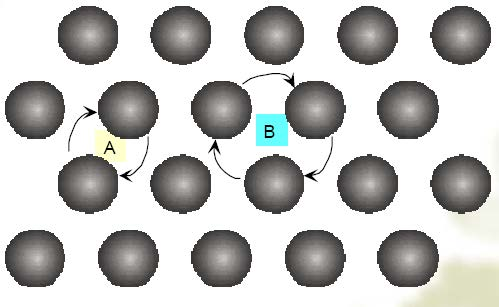
\includegraphics[width=0.5\textwidth]{fig/ring_diffusion.jpg}
                \caption{环行扩散的两种机制,其中A为直接交换,B为循环交换。}
                \label{环行扩散的两种机制}
            \end{figure}
        \subsection{空位扩散}
            \textbf{空位扩散}\index{空位扩散}对于晶体中存在的空位,空位周围的原子都是向空位进行扩散,
            扩散后形成新的空位。
        \subsection{挤列扩散}
            \textbf{挤列扩散}\index{挤列扩散}是在$n$个原子位置上挤进去一个原子,容纳了$n+1$个原子位置上挤进去一个原子,容纳了并作为
            一个整体沿挤列方向扩散。由于碱金属原子的压缩性较大,有可能形成这种组态。
    \section{Fick定律及其应用}
        \subsection{Fick第一定律}
            Fick 认为原子的扩散有具体的方向,应当从高浓度向低浓度扩散,以此得到了稳态下的Fick第一定律
            \begin{equation}
                J=-D\left( \frac{\partial c}{\partial x} \right)\label{Fick第一定律},
            \end{equation}
            上式称为\textbf{Fick第一定律}\index{Fick第一定律} ,其中 $J$为\textbf{扩散通量}\index{Fick第一定律!扩散通量},
            是某一时刻通过垂直于$x$轴的单位平面原子的通量;\textbf{扩散系数}\index{Fick第一定律!扩散系数}
            表示单位浓度梯度下的通量,上式表明,扩散方向与梯度方向相反。
            习惯上,\autoref{Fick第一定律}中各个量的单位为
            \begin{table}[ht]
                \centering
                \caption{Fick第一定律中各个物理量单位。}
                \label{Fick第一定律中各个物理量单位}
                \begin{tabular}{cc}
                    \toprule
                    物理量&单位\\
                    \midrule
                    $J$&\si{\g\per(\s\cdot\cm^2)}\\
                    $D$&\si{\cm^2\per\s}\\
                    $c$&\si{\g\per\cm^3}\\
                    $x$&\si{\cm}\\
                    \bottomrule
                \end{tabular}
            \end{table}
            
            对于三维空间,第一定律可以写作
            \begin{equation}
                J=-D\nabla c.
            \end{equation}
        \subsection{Fick第二定律}
            但是实际上,扩散通量$J$一般是不稳定的,伴随$x$变化,因此不同位置的浓度也会不同,
            对于$x_1$位置的$\dif x$厚度的体积元,单位时间的净通量为$J(x_1)-J(x_1+\dif x)$,
            其浓度改变速率为$\partial c/\partial t$,则有如下关系
            \begin{equation}
                \left( \frac{\partial c}{\partial t} \right)_{x_1}\dif x=J(x_1)-J(x_1+\dif x),
            \end{equation}
            当$\dif x\to0$时,有
            \begin{equation}
                J\left(x_{1}+\dif x\right)=J\left(x_{1}\right)+\left(\frac{\partial J}{\partial x}\right)_{x 1} \dif x
            \end{equation}
            所以有
            \begin{equation}
                \frac{\partial c}{\partial t}=-\frac{\partial J}{\partial x}=\frac{\partial}{\partial x}\left(D \frac{\partial c}{\partial x}\right),
            \end{equation}
            上式就是\textbf{Fick第二定律}\index{Fick第二定律}。
        
            一维情况下对于扩散系数$D$为常数的情况,Fick第二定律可以写作
            \begin{equation}
                D\left(\frac{\partial^{2} c}{\partial x^{2}}\right)=\frac{\partial c}{\partial t},
            \end{equation}
            对于扩散系数为变量的情况,Fick第二定律写作
            \begin{equation}
                \frac{\partial}{\partial x}\left[D\left(\frac{\partial c}{\partial x}\right)\right]=\frac{\partial c}{\partial t}.
            \end{equation}
            
            对于三维空间,在笛卡尔坐标系下,使用拉普拉斯算子,Fick第二定律可以写作
            \begin{equation}
                D\left(\frac{\partial^{2} c}{\partial x^{2}}+\frac{\partial^{2} c}{\partial y^{2}}+\frac{\partial^{2} c}{\partial z^{2}}\right)=\frac{\partial c}{\partial t}.
            \end{equation}

        \subsection{扩散方程的解}
            对于不同的类型,可以分为稳态扩散和非稳态扩散,其中\textbf{稳态扩散}\index{稳态扩散}
            是指空间各点的浓度不随时间发生变化,这种状态称为稳态扩散;\textbf{非稳态扩散}\index{非稳态扩散}是指
            空间中各点浓度随时间发生变化。
            \subsubsection{第一类稳态扩散}
                首先来看稳态扩散,假设扩散系数为常数,浓度不随时间发生变化。
                容器中间有金属薄板,薄板的一面保持高而恒定的浓度,另一面保
                持低而恒定的浓度,因此在金属板中存在浓度梯度。假设器壁不可渗透,
                经过一段时间,薄板中任一体积元,流入的和流出的通量相等,扩散达
                到稳定状态。
                
                此时的边界条件为$x=0$,$c=c_1$,$x=\Delta x$时,$c=c_0$,金属薄板的面积为$A$,
                总扩散通量为
                \begin{equation}
                    J_{\text{total}}=-AD\frac{\partial c}{\partial x},
                \end{equation}
                由于问题属于一维问题,可以将偏微分改为全微分
                \begin{equation}
                    J_{\text{total}}=-AD\frac{\dif c}{\dif x},
                \end{equation}
                两边同时乘以$\dif x$并在$0\to\dif x$范围内积分,有
                \begin{equation}
                    \int_{0}^{\Delta x}J_{\text{total}}\dif x=-\int_{c_{1}}^{c_{0}} A D \dif c
                \end{equation}
                得到
                \begin{equation}
                    J_{\text{total}}=\frac{AD(c_1-c_0)}{\Delta x}.
                \end{equation}

                这一类模型可以模拟钢铁真空脱气,假设金属表面溶解度与相接触的气体压力有关,对于
                双原子气体有
                \begin{equation}
                    c=S\sqrt{p},
                \end{equation}
                单位面积的扩散通量就可以写作
                \begin{equation}
                    J=\frac{D S\left(\sqrt{p_{1}}-\sqrt{p_{0}}\right)}{\Delta x}.
                \end{equation}
            \subsubsection{第二类稳态扩散}
                这类问题扩散是指空间各点的浓度不随时间发生变化,但是扩散系数$D$不是常数。
                有人利用这一特点模拟了碳在$\gamma$铁中的扩散过程并测量了扩散系数。

                将长度为$l$、半径为$r$的薄壁铁管在\SI{1000}{\celsius}下退火,管内
                是渗碳气氛,关外是脱碳气氛,当时间最够长时,壁管内各点的碳浓度不再随时间而变,
                也就是
                \begin{equation}
                    \frac{\partial c}{\partial t}=0.
                \end{equation}
                达到稳定状态后,设$t$时间内通过管壁的碳量为$q$,则单位时间通过
                的碳量$q/t$为常量。因而,单位时间流入或流出单位面积的通量为
                \begin{equation}
                    J=\frac{q}{2\pi lt},
                \end{equation}
                根据\autoref{Fick第一定律}可得
                \begin{equation}
                    \frac{q}{2\pi lt}=-D\frac{\dif c}{\dif r},
                \end{equation}
                解得
                \begin{equation}
                    q=-D\left( 2\pi lt \right)\frac{\dif c}{\dif \ln r},
                \end{equation}
                式中,$q$,$l$,$t$以及碳沿管壁的径向分布都可以测量,扩散系数$D$
                可以由$c$对$\ln r$的斜率确定。

            \subsubsection{第一类非稳态扩散}
                这种情况是空间各点的浓度随时间发生变化,但是$D$为常数的情况,
                此时的Fick第二定律可以写作
                \begin{equation}
                    \frac{\partial c}{\partial t}=D \frac{\partial^{2} c}{\partial x^{2}}.
                \end{equation}
                这一公式可以解决两种模型,分别为\textbf{瞬时平面源}\index{瞬时平面源}和\textbf{一维半无限模型}\index{一维半无限模型}(也称为叠加法)。

                对于瞬时平面源模型,假设两块足够长的相同纯金属,其中
                一块端面上涂上同位素(作为扩散面源),对接起来组成扩散偶,假设扩散系数为常数
                Fick第二定律的解的形式为
                \begin{equation}
                    c=\frac{A}{\sqrt{t}} \exp \left(-\frac{x^{2}}{4 D t}\right),
                \end{equation}
                式中$A$为待定系数。由于扩散总量一定,为$M$,也就是
                \begin{equation}
                    \int_{-\infty}^{\infty} c(x, t) \mathrm{d} x=M,
                \end{equation}
                可以解得
                \begin{equation}
                    c(x, t)=\frac{M}{2 \sqrt{\pi D t}} e^{-\frac{x^{2}}{4 D t}}
                \end{equation}

                对于另一种模型,则是假设一块无限长的金属,$x<0$为扩散源,$x>0$为被扩散物质。
                首先求解单位体积元扩散对$x>0$的某一点的影响,该点的总浓度就是所有体积元作用的总和。
                求解过程相对复杂,这里直接给出结果
                \begin{equation}
                    c(x, t)=\frac{c_{0}}{2}\left[1-\operatorname{erf}\left(\frac{x}{2 \sqrt{D t}}\right)\right]
                \end{equation}
                其中$\operatorname{erf}$为误差函数,其有数值表可以查阅。
                假设初始浓度为$c=c_0$,扩散时,表面浓度恒定为$c=c_s$,则上式可以写作
                \begin{equation}
                    c(x,t)=c_0+(c_s-c_0)\left[ 1-\operatorname{erf}\left( \frac{x}{2\sqrt{Dt}} \right) \right],
                \end{equation}
                这一公式适用于工业上工件的渗碳过程。

                这里还有一个概念性的常用关系式,当某一处的浓度满足
                \begin{equation}
                    \frac{c-c_{0}}{c_{s}-c_{0}}=\frac{1}{2},
                \end{equation}
                该处对应的位置为
                \begin{equation}
                    x_{\frac{1}{2}}=\sqrt{Dt},
                \end{equation}
                这一位置的$x$称为\textbf{半浓度深度}\index{Fick第二定律!半浓度深度},记作$x_{1/2}$,
                对与任意时间都成立。

                对于温度改变的系统,测量此时的\textbf{扩散系数}\index{Fick第二定律!扩散系数} ,可以发现其与温度有明显的关系,一般可以写作
                \begin{equation}
                    D=D_0\exp\left( -\frac{Q}{RT} \right),
                \end{equation}
                上式称为\textbf{Arrhenius关系}\index{Fick第二定律!扩散系数!Arrhenius关系},其中$Q$为
                扩散激活能,式中$Q$、$D_0$与温度无关,与成分、结构有关。
            \subsubsection{第二类非稳态扩散}
                这一类问题研究$D$随浓度变化的全无限长的一维扩散。如果将铜和
                黄铜对接起来,组成浓度差很大的扩散偶,则D因浓度而变。\ce{Zn}的浓度初始分布为
                $x>0$,$c=c_0$,$x<0$,$x=0$,对此解偏微分方程
                \begin{equation}
                    \frac{\partial c}{\partial t}=\frac{\partial }{\partial x}\left( D\frac{\partial c}{\partial x} \right),
                \end{equation}
                某处浓度为$c_1$,求得其扩散系数
                \begin{equation}
                    D_{c_1}=-\frac{1}{2t}\left.\frac{\dif x}{\dif c}\right\vert_{c=c_1}\cdot\int_{0}^{c_1}x\dif c\label{扩散系数随浓度变化关系},
                \end{equation}
                式中$\frac{\dif x}{\dif c}\vert_{c=c_1}$为$c-x$曲线上$c=c_1$处的斜率,$\int_{0}^{c_1}x\dif c$为积分面积。
                这样可以解决扩散系数问题,但是$\int_{0}^{c_1}x\dif c$中,$x$的原点不一定是是原始的焊接面,
                因此在求解扩散系数时必须先确定\textbf{Matano面}\index{Matano面} ,也就是在这个面两侧的$c-x$曲线积分面积相等,
                也就是$\int_{0}^{c_1}x\dif c=0$,为了区分Matano面和原始焊接面,后者记作$x'=0$。因此在
                实际中求解某处的扩散系数一般要四步
                \begin{itemize}
                    \item[1] 在一定温度$T$下,是扩散偶退火一定时间$t$,分析浓度$c$,作出$c-x$曲线;
                    \item[2] 使两边积分面积相等,确定Matano面;
                    \item[3] 求$c_1$处的切线斜率和积分面积$\int_{0}^{c_1}x\dif c$;
                    \item[4] 代入\autoref{扩散系数随浓度变化关系},求出$D_{c_1}$。
                \end{itemize}

                关于Matano面,有以下两点结论:
                \begin{itemize}
                    \item[1] 扩散过程中,体积保持不变时,焊接面和Matano面一致;
                    \item[2] Matano面分割物质的流动体积,使一边流出的物质量等于另一边流入的量。
                \end{itemize}
            \subsubsection{均匀化速率问题}
                在实际中,经常遇到不均匀合金的均匀化问题,如奥氏体化时第
                二相的溶解速度问题,铸态合金的均匀化问题\index{均匀化问题}等。

                在不均匀合金中,如果浓度沿某一方向呈周期性变化,则合金的初始浓度分布可以用下式来表示
                \begin{equation}
                    c(x)=c_0+c_m\cos\left( \frac{\pi x}{l} \right).
                \end{equation}
                对于这一类问题的Fick方程的解为
                \begin{equation}
                    c(x, t)=c_{0}+c_{m} \cos \left(\frac{\pi x}{l}\right) \exp \left(-\frac{t}{\tau}\right),
                \end{equation}
                其中$\tau=\frac{l^2}{\pi^2D}$称为\textbf{弛豫时间}\index{均匀后问题!弛豫时间}。减少弛豫时间
                可以加速体系均匀化,可以采用升高温度或减少长度的方法,由于温度的改变导致扩散系数的改变对结果的影响
                不大,因此主要采用减少长度的方法,因此需要快冷、锻打。
    
    \section{原子迁移和扩散系数}
        \subsection{扩散系数的统计性}   
            扩散的宏观现象是由大量原子的无数次随机行走造成的。只有用统计概念才能计算扩散系数。
            之前的Fick定律认为体系的扩散方向为顺浓度方向,然而实际中还存在着"上坡"扩散这样的
            例外,这只能从能量角度来解释,也就是说,扩散的真正驱动力为化学位梯度而不是浓度梯度。

            对于两个临近晶面,原子面密度分别为$n_1$和$n_2$,假设每次迁移的距离都是$\alpha$,
            一个原子单位时间内迁移$\Gamma$次,则$\delta t$时间内从面1跳出的原子数为
            $n_1\Gamma\delta t$。如果迁移方向是随机的,对于三维问题,则从晶面1迁移
            到晶面2的概率就是$1/6$,在$\delta t$时间内从1跳到2的原子数为$\frac{1}{6}n_1\Gamma\delta t$,
            同理从2跳到1的原子数为$\frac{1}{6}n_2\Gamma\delta t$,则面1到面2的净通量为
            \begin{equation}
                J=\frac{1}{6}(n_1-n_2)\Gamma\label{迁移通量与面密度关系},
            \end{equation}
            面密度和浓度的关系为
            \begin{equation}
                \frac{n}{\alpha}=c,
            \end{equation}
            因此净通量写作
            \begin{equation}
                J=\frac{1}{6}\alpha\left( c_1-c_2 \right)\Gamma.
            \end{equation}
            由于
            \begin{equation}
                \frac{\partial c}{\partial x}=\frac{c_2-c_1}{\alpha},
            \end{equation}
            得到
            \begin{equation}
                J=-\frac{1}{6}\alpha^2\Gamma\frac{\partial c}{\partial x},
            \end{equation}
            与Fick第一定律比较得到
            \begin{equation}
                D=\frac{1}{6}\alpha^2\Gamma\label{扩散系数与迁移率和迁移距离关系},
            \end{equation}
            可知扩散系数正比于迁移率和迁移距离的平方。
            从以上的讨论也可以看出,决定迁移净通量的是不同原子面之间的面密度而不是浓度梯度。

            对于fcc和hcp金属来说,在熔点附近的迁移率为\SI{1e8}{\s^{-1}},但是实际上原子热振动频率为
            \numrange{1e12}{1e13},原子在平衡位置振动\numrange{1e4}{1e5}次才会成功跳离一次。

            一般来说,迁移距离随温度的变化不大,这只和点阵类型和点阵常数有关系,扩散速率
            与温度的关系主要取决于迁移率$\Gamma$,假设
            \begin{equation}
                \Gamma=Zp_v\omega,
            \end{equation}
            其中$Z$为配位数,$p_v$为近邻是空位置的几率,$\omega$原子迁入空位的频率,
            代入\autoref{扩散系数与迁移率和迁移距离关系}可得
            \begin{equation}
                D=\frac{1}{6}\alpha^2Zp_v\omega.
            \end{equation}

    \section{扩散系数与浓度}
        \subsection{Kirkendall效应}
            这里不再叙述\href{http://www.phase-trans.msm.cam.ac.uk/kirkendall.html}{Kirkendall效应}\index{Kirkendall效应}的实验过程,
            直接说明结论,对于由A、B两种原子组成的体系,$D_A>D_B$引起的\textbf{标记面}\index{Kirkendall效应!标记面}的移动称为Kirkendall效应。
            其不可能使用原子交换机制进行迁移,因为如果扩散使用原子交换进行,对于任意平面来说,净通量
            都为零。
        \subsection{Darken公式}
            A、B原子的百分比分别为$N_1=c_1/c$、$N_2=c_2/c$,扩散系数分别为$D_1$、$D_2$,
            标记面移动速度为$V$,得出\textbf{Darken公式}\index{Darken公式}
            \begin{align}
                \widetilde{D}&=N_{2} D_{1}+N_{1} D_{2},\\
                v&=\left(D_{2}-D_{1}\right) \frac{\partial N_{2}}{\partial x},\\
                v&=\left(D_{1}-D_{2}\right) \frac{\partial N_{1}}{\partial x}
            \end{align}
            以上三式合称Darken公式。在一定浓度下测得化学扩散系数$\widetilde{D}$、标记面移动速度$V$
            和浓度梯度,就可以确定该浓度下的\textbf{偏扩散系数}\index{偏扩散系数}$D_1$、$D_2$,它们是浓度梯度下
            组元的扩散系数,称$\widetilde{D}$为\textbf{化学扩散系数}\index{Darken公式!化学扩散系数}或互扩散系数。

        \subsection{总结}
            目前已经接触了三个平面,分别是原始焊接平面($S_0$)\index{原始焊接平面},Matano面($S_M$)\index{Matano面}
            和标记面($S_I$)\index{Kirkendall效应!标记面},这里总结在不同条件下它们的相对位置的变化,
            从而建立扩散过程中物质流动的明确图像。
            \begin{itemize}
                \item[1] 当$\frac{\dif c}{\dif t}=0$,且$D_1=D_2$时,$V=0$,所以$S_0=S_I$,而且$J_1=-J_2$,所以$S_0=S_M$,三个面重合;
                \item[2] 当$\frac{\dif c}{\dif t}=0$,$D_1\neq D_2$时,$J_1\neq J_2$,$S_I\neq S_0$,但是$S_0=S_m$;
                \item[3] 当$\frac{\dif c}{\dif t}\neq0$,$D_1=D_2$时,$S_0\neq S_M$,但是$S_I=S_M$;
                \item[4] 当$\frac{\dif c}{\dif t}\neq0$,且$D_1\neq D_2$时,三个面均不相等。
            \end{itemize}
            总结一下,偏扩散系数相等时,标记面和Matano面相等;空间中浓度不随时间发生变化时,焊接面和Matano面相等。

            关于Fick定律和Kirkendall效应有以下几点说明
            \begin{itemize}
                \item 每一种原子都有其自身的本征扩散系数;
                \item 原子成功跃迁的几率依赖于结合键被拆断的难易程度,因此与金属的熔点有关;
                \item 扩散的全部结论,或者说Fick定律中的扩散系数是不同种类原子本征扩散的综合作用的函数,即Darken公式;
                \item 由于不同的本征扩散系数,Fick定律中的扩散系数是成分的函数。Matano面的构架是评价扩散系数对浓度的依赖性的一个方法;
                \item 由于本征扩散系数不同,在扩散偶中存在空位的净通量。当两边的空位各自重新排列趋向平衡时,两边的合金就改变了相对体积。这引起了界面移动,即Kirkendall效应;
                \item 跃迁频率和扩散系数之间的简单关系对自扩散是有效的,对稀固溶体是很好的近似。
            \end{itemize}
    \section{反应扩散}
        在许多合金状态图中有中间相,因而扩散过程中也可能出现中间相,这种扩散即为\textbf{多相扩散}\index{多相扩散}。

        多相扩散包括两个过程,分别是扩散过程和界面上达到一定的浓度发生化学反应,从而形成新相的过程。

        通过扩散使固溶体内的溶质组元超过固溶度限而不断形成新相的过程就是\textbf{反应扩散}\index{反应扩散}由反应扩散所产生的新相,可以是新的固
        溶体,也可以是化合物。

        反应扩散的特点是在相界面处产生浓度突变,突变的浓度正好对应于相的极限溶解度。
        根据相律关系,自由度$F$、族元数$C$和相数$P$关系为
        \begin{equation}
            F=C-P+2,
        \end{equation}
        但是在扩散过程中,温度和压力一定,因此应当去掉两个自由度,此时$F=C-P$,
        \begin{itemize}
            \item 单相情况下,$P=1$,$C=2$,于是$F=2-1=1$,说明该相的浓度是可以改变的,因此在扩散过程中可以有浓度梯度,即扩散过程可以发生;
            \item 在双相去,$F=2-2=0$,意味着在双相区中,各相的浓度不能改变,它与状态图中的极限溶解度相对应,说明在两相区中不存在浓度梯度。
        \end{itemize}
        
        \subsection{新相长大的动力学}
            由纯金属A、B组成的扩散偶,在各自的\textbf{边际固溶体}\index{一次固溶体!边际固溶体}中存在有
            极限溶解度。经过时间$t$后的浓度分布曲线为
	\chapter{相变}
    \section{相变概念}
        关于相变,有一些最为基础的概念,
        \begin{enumerate}
            \item 相\index{相}:成分相同、结构相同,有界面同其他部分分隔的物质均匀组成部分;
            \item 相变\index{相变}:当外界条件(如温度、压力等)连续变化时,物质自身发生突变的现象。或物相的某个(阶)热力学势跃变,伴随物相的某个(些)要素跃变;
            \item 固态相变\index{固态相变}:固体材料的结构在温度、压力、成分改变时所发生的转变。
        \end{enumerate}

        在分类上,有很多种分类方法,比如从动力学上,或者是从热力学上分类
            \subsection{动力学相变分类}
                相变分为两类:扩散性和无扩散型,如\autoref{金属及合金中的一级相变}所示。
                无扩散型相变\index{无扩散型相变}较为简单,分为连续型相变\index{连续型相变},比如$\omega$相比\index{$\omega$相变},和形核长大型相变\index{形核长大型相变},比如马氏体相变\index{马氏体相变}。

                而扩散性相变\index{扩散性相变}则相对复杂,也分为连续型相变\index{连续型相变}和形核长大型相变\index{形核长大型相变},更为具体的分类将在后面的章节进行讲解,在这里不再进行过多叙述。
                \begin{figure}[ht]
                    \centering
                    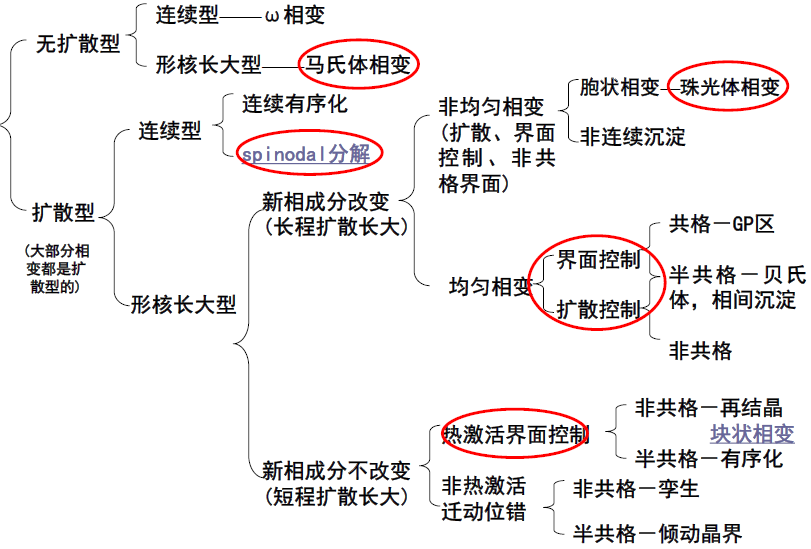
\includegraphics[width=0.7\textwidth]{fig/first_phase_transformation_in_alloys.png}
                    \caption{金属及合金中的一级相变。}
                    \label{金属及合金中的一级相变}
                \end{figure}
            \subsection{热力学的相变分类}
                在热力学的分类比较简单,分为一级相变\index{一级相变}和二级相变\index{二级相变}。
                一级相变是指化学位相等,但是化学位的一阶导数不等,也就是熵不等或者是体积不等,
                \begin{align}
                    \mu_1&=\mu_2,\\
                    \left(  \frac{\partial\mu_1}{\partial T} \right)_p=-S_1&\neq-S_2= \left(  \frac{\partial\mu_2}{\partial T} \right)_p\label{等压一级相变},\\
                    \left(  \frac{\partial\mu_1}{\partial p} \right)_T=V_1&\neq V_2= \left(  \frac{\partial\mu_2}{\partial p} \right)_T\label{等温一级相变}.
                \end{align}
                在一级相变中伴有能量变化,或者吸热或者放热,或者体积发生变化。比如晶体的熔化、升华、液体的凝固、汽化、气体的凝聚以及晶体中大多数晶型转变都属于一级相变,这是最普遍的相变类型。

                二级相变是指化学位的二阶导数发生突变,而化学位和一阶导数不发生突变,
                \begin{align}
                    -\frac{C_p}{T}=\left(  \frac{ \partial^2\mu_1  }{\partial T^2} \right)_p&\neq\left(  \frac{ \partial^2\mu_2  }{\partial T^2} \right)_p,\\
                    kV=\left(  \frac{ \partial^2\mu_1  }{\partial p^2} \right)_T&\neq\left(  \frac{ \partial^2\mu_2  }{\partial p^2} \right)_T,\\
                    \alpha V=\frac{\partial^2\mu_1}{\partial T\partial p}&\neq\frac{\partial^2\mu_2}{\partial T\partial p}.
                \end{align}
                其中$C_p$为等压比热\index{等压比热},$k$为等温等压系数\index{等温等压系数},$\alpha$为等压膨胀系数\index{等压膨胀系数}\footnote{熔化、马氏体转变属一级相变,有序化可能是一级也
                可能是二级相变。}。
                在二级相变中,两相的化学势、熵和体积相等,但热容、膨胀系数和压缩系数不相等,即无相变潜热,无体积的突变,只有热容、
                膨胀系数和压缩系数的不连续变化,
                \begin{align*}
                    \Delta C_p\neq 0,\\
                    \Delta\beta\neq 0,\\
                    \Delta\alpha\neq0.\\
                \end{align*}
                一般合金的有序-无序转变、铁磁-顺磁转变、超导转变等属于二级相变。大多数便随某种物理性能的变化。
            \subsection{固溶体自由能的计算}
                纯组元的自由能和温度的关系可以写作
                \begin{equation}
                    G(T)=H(T)-TS(T),
                \end{equation}
                而两相混合的自由能,在理想条件下可以由两相的自由能叠加得到。

                假设在体系中存在两种相$\alpha$和$\beta$,均是由A、B两种原子构成,假设A原子的成分为$x\mathrm{at.}\%$,在$\alpha$相中,A的原子百分比为$x_1$,在$\beta$中的原子百分比为$x_2$
                而$\alpha$相和$\beta$的占比分别为$N_1$和$N_2$,两者的自由能分别为$G_1$和$G_2$,混合后的自由能为
                \begin{equation}
                    G=N_1G_1+N_2G_2,
                \end{equation}
                利用成分关系,可以变为
                \begin{equation}
                    G=G_1+\frac{x-x_1}{x_2-x_1}(G_2-G_1),
                \end{equation}
                所以$G_1$,$G$,$G_2$处于同一直线,并且服从杠杆定律。

                但是在混合过程存在其他作用,导致混合后的自由能不等于理想情况下的自由能。这里假设实际的自由能为
                \begin{equation}
                    G(x)=G^0+\Delta G^m,
                \end{equation}
                其中
                \begin{equation}
                    G^0=x_AG_A^0+x_BG_B^0,
                \end{equation}
                其中,$x_A$为$A$原子的原子百分比,$x_B$为$B$原子的原子百分比,而要计算$\Delta G^m$,需要先计算混合过程中的焓\index{焓}和熵\index{熵}的变化量。
                \subsubsection{混合过程中熵的改变量}
                    固态下的系统的熵主要由混合熵\index{熵!混合熵}(决定于原子可能排列的方式)和振动熵\index{熵!振动熵}(决定于温度和缺陷)组成,
                    混合熵的变化为
                    \begin{equation}
                        \Delta S^m=S_{AB}-(x_AS_A+x_BS_B),
                    \end{equation}
                    根据混合熵的定义
                    \begin{equation}
                        S=k\ln{\Omega},
                    \end{equation}
                    其中$k$为玻尔兹曼常数,$\Omega$为微观状态数,假设$A$的原子数为$N_A$,$B$的原子数为$N_B$,混合熵的变化为
                    \begin{equation}
                        \begin{split}
                        \Delta S^m&=S_{AB}-(x_AS_A+x_BS_B)\\
                        &=k\ln{\frac{N!}{N_A!(N-N_A)!}}-x_Ak \ln \left(C_{N_{A}}^{N_{A}}\right)  -x_Bk \ln \left(C_{N_{B}}^{N_{B}}\right)\\
                        &=k\ln{\frac{N!}{N_A!N_B!}}\\
                        &=k\left( \ln{N!}-\ln{N_A!}-\ln{N_B!} \right).                
                        \end{split}                                      
                    \end{equation}
                    根据Stirling公式,
                    \begin{equation}
                        \Delta S^m=-R(x_A\ln{x_A}+x_B\ln{x_B}),
                    \end{equation}
                    其中$R=kN$。
                \subsubsection{混合过程中焓的改变量}
                    接下来计算混合过程中焓的变化,利用溶液的准化学模型\index{准化学模型},假设
                    \begin{enumerate}
                        \item $A$,$B$两组元尺寸接近,排列无序;
                        \item 混合过程中体积基本不变,即$\Delta V=0$;
                        \item 原子只与最近邻的原子之间存在相互作用,即只计算最近邻原子之间的结合能。
                    \end{enumerate}
                    假设两个近邻原子之间额定结合能分别为$u_{AA}$、$u_{AB}$和$u_{BB}$,固溶体和组元的配位数均为$Z$。在恒压情况下,焓的改变仅与结合能的改变有关,
                    所以
                    \begin{align}
                        \text{混合前,}&u_{1}=\frac{1}{2} N_{A} Z u_{A A}+\frac{1}{2} N_{B} Z u_{B B},\\
                        \text{混合后,}&u_{2}=\frac{1}{2} N_{A} Z \frac{N_{A}}{N} u_{A A}+\frac{1}{2} N_{B} Z \frac{N_{B}}{N} u_{B B}+N_{A} Z \frac{N_{B}}{N} u_{A B}.
                    \end{align}
                    所以焓的变化量为
                    \begin{equation}
                        \Delta u^m=Z N\left(u_{A B}-\frac{u_{A A}+u_{B B}}{2}\right) x_{A} x_{B},
                    \end{equation}
                    令$\alpha'=ZN\left( u_{AB}-\frac{u_{AA}+u_{BB}}{2} \right)$,焓变可以写作
                    \begin{equation}
                        \Delta H^m=\alpha'x_Ax_B.
                    \end{equation}
            \subsection{混合过程的自由能改变量以及成分与自由能关系}
                所以混合过程中自由能随成分和温度变化的关系为
                \begin{equation}
                    G(x)=G_{A}^{0} x_{A}+G_{B}^{0} x_{B}+\alpha^{\prime} x_{A} x_{B}+R T\left(x_{A} \ln x_{A}+x_{B} \ln x_{B}\right)\label{混合过程的自由能曲线}.
                \end{equation}
                下面将对于这一曲线进行讨论。

                混合前的自由能为$G_{A}^{0} x_{A}+G_{B}^{0} x_{B}$为一条直线,而熵的改变量则由于成分百分比均小于1而小于0,但是$\alpha^{\prime}$,也就是原子结合能的改变量不是能够确定的事,需要分情况讨论。
                在此之前,先进一步确定曲线与成分的关系,
                \begin{align}
                    \frac{\partial G}{\partial x_{B}}&=-G_{A}^{0}+G_{B}^{0}+\alpha^{\prime}\left(x_{A}-x_{B}\right)+R T\left(\ln x_{B}-\ln x_{A}\right),\\
                    \frac{\partial^{2} G}{\partial x_{B}^{2}}&=-2 \alpha^{\prime}+R T\left(\frac{1}{x_{A}}+\frac{1}{x_{B}}\right).
                \end{align}
                由此可见,曲线中唯有成分也就是结合能的变化不能确定,下面将针对结合能变化的三种情况进行讨论。

                当原子结合能不发生改变时,也就是$\alpha^{\prime}=0$时,此时体系符合理想溶液模型,自由能的二阶导数
                \begin{equation}
                    \frac{\partial^{2} G}{\partial x_{B}^{2}}=R T\left(\frac{1}{x_{A}}+\frac{1}{x_{B}}\right)>0,
                \end{equation}
                $G(x)$为下垂线,及曲线的凹向朝上,如\autoref{混合时结合能不变的自由能曲线}所示。
                \begin{figure}[ht]
    \centering
    %\begin{subfigure}[0.3\textwidth]
    \subfloat[混合时结合能不变的自由能曲线]
    {
        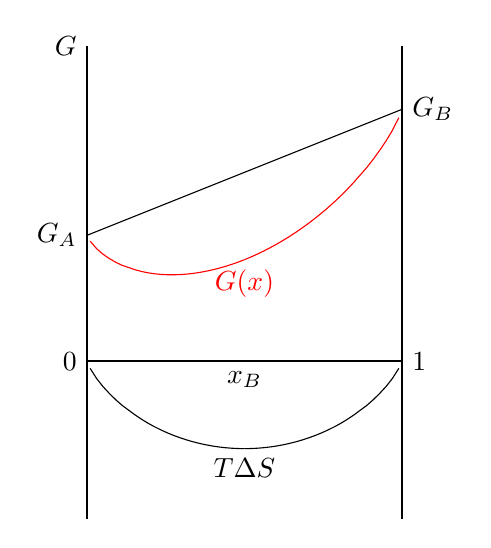
\begin{tikzpicture}[scale=4]
            \draw[thick] (0,0) node[anchor=east]{0} --(0.5,0) node[anchor=north] {$x_B$}--(1,0) node[anchor=west]{1};
            \draw[thick] (0,-0.5) -- (0,0.4) node[anchor=east]{$G_A$}--(0,1) node[anchor=east]{$G$};
            \draw[thick] (1,-0.5) -- (1,0.8) node[anchor=west]{$G_B$}--(1,1);
            
            \draw[thin] (0,0.4)--(1,0.8);
            \draw[domain=0.01:0.5] plot(\x,{0.4*(\x*ln(\x)+(1-\x)*ln((1-\x)))})
                node[below] {$T\Delta S$};
            \draw[domain=0.5:0.99] plot(\x,{0.4*(\x*ln(\x)+(1-\x)*ln((1-\x)))});
            %G(x)
            \draw[red,domain=0.01:0.5] plot(\x,{0.4*\x+0.4+0.4*(\x*ln(\x)+(1-\x)*ln((1-\x)))})
                node[below] {$G(x)$};
            \draw[red,domain=0.5:0.99] plot(\x,{0.4*\x+0.4+0.4*(\x*ln(\x)+(1-\x)*ln((1-\x)))});        
        \end{tikzpicture}
       % \caption{$\Delta H^M=0$,混合时结合能不变的自由能曲线。}
        \label{混合时结合能不变的自由能曲线}
    }
   % \end{subfigure}
   % \begin{subfigure}[0.3\textwidth]
    \subfloat[混合时结合能减小的自由能曲线]
    {
           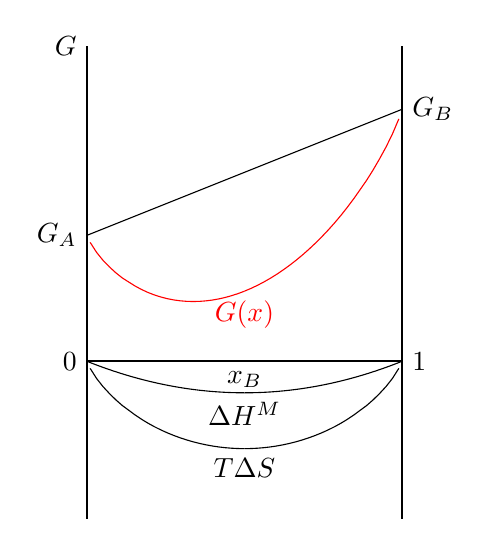
\begin{tikzpicture}[scale=4]
            \draw[thick] (0,0) node[anchor=east]{0} --(0.5,0) node[anchor=north] {$x_B$}--(1,0) node[anchor=west]{1};
            \draw[thick] (0,-0.5) -- (0,0.4) node[anchor=east]{$G_A$}--(0,1) node[anchor=east]{$G$};
            \draw[thick] (1,-0.5) -- (1,0.8) node[anchor=west]{$G_B$}--(1,1);
            %G(0)
            \draw[thin] (0,0.4)--(1,0.8);
            %T\Delta S
            \draw[domain=0.01:0.5] plot(\x,{0.4*(\x*ln(\x)+(1-\x)*ln((1-\x)))})
                node[below] {$T\Delta S$};
            \draw[domain=0.5:0.99] plot(\x,{0.4*(\x*ln(\x)+(1-\x)*ln((1-\x)))});
            %\Delta H
            \draw[domain=0:0.5] plot(\x,{-0.4*(\x*(1-\x))})
                node[below] {$\Delta H^M$};
            \draw[domain=0.5:1] plot(\x,{-0.4*(\x*(1-\x))});
            
            %G(x)
            \draw[red,domain=0.01:0.5] plot(\x,{0.4*\x+0.4-0.4*(\x*(1-\x))+0.4*(\x*ln(\x)+(1-\x)*ln((1-\x)))})
                node[below] {$G(x)$};
            \draw[red,domain=0.5:0.99] plot(\x,{0.4*\x+0.4-0.4*(\x*(1-\x))+0.4*(\x*ln(\x)+(1-\x)*ln((1-\x)))});        
        \end{tikzpicture}
        %\caption{$\Delta H^M<0$,混合时结合能小于零的自由能曲线。}
        \label{混合时结合能减小的自由能曲线}
    }
    
    %\end{subfigure}
    \caption{两种不同情况的自由能曲线}
\end{figure}


                当焓变小于零时,也就是$\Delta H^M<0$,
                \begin{equation}
                    \frac{\partial^{2} G}{\partial x_{B}^{2}}=2 \alpha^{\prime}+R T\left(\frac{1}{x_{A}}+\frac{1}{x_{B}}\right)<0,
                \end{equation}
                这时异类原子的结合力大于同类原子之间的结合力。表现为在溶解时会放出热量。此时$G(x)$为下垂线,曲线的凹陷更大,如\autoref{混合时结合能减小的自由能曲线}所示。

                当焓变大于零时,焓变与熵的变化为相反的作用,曲线的形状与两者的大小有关。
                
                
                \begin{figure}[ht]
    \centering
    %\begin{subfigure}[0.3\textwidth]
    \subfloat[$T>\frac{\alpha^{\prime}}{2R}$]
    {
        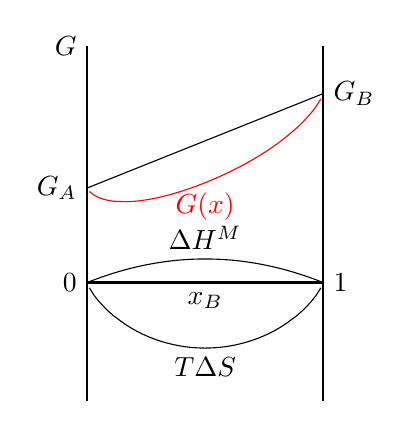
\begin{tikzpicture}[scale=3]
            \draw[thick] (0,0) node[anchor=east]{0} --(0.5,0) node[anchor=north] {$x_B$}--(1,0) node[anchor=west]{1};
            \draw[thick] (0,-0.5) -- (0,0.4) node[anchor=east]{$G_A$}--(0,1) node[anchor=east]{$G$};
            \draw[thick] (1,-0.5) -- (1,0.8) node[anchor=west]{$G_B$}--(1,1);
            
            \draw[thin] (0,0.4)--(1,0.8);
            \draw[domain=0.01:0.5] plot(\x,{0.4*(\x*ln(\x)+(1-\x)*ln((1-\x)))})
                node[below] {$T\Delta S$};
            \draw[domain=0.5:0.99] plot(\x,{0.4*(\x*ln(\x)+(1-\x)*ln((1-\x)))});
            
            %\Delta H
            \draw[domain=0:0.5] plot(\x,{0.4*(\x*(1-\x))})
                node[anchor=south] {$\Delta H^M$};
            \draw[domain=0.5:1] plot(\x,{0.4*(\x*(1-\x))});
            
            %G(x)
            \draw[red,domain=0.01:0.5] plot(\x,{0.4*\x+0.4+0.4*(\x*(1-\x))+0.4*(\x*ln(\x)+(1-\x)*ln((1-\x)))})
                node[below] {$G(x)$};
            \draw[red,domain=0.5:0.99] plot(\x,{0.4*\x+0.4+0.4*(\x*(1-\x))+0.4*(\x*ln(\x)+(1-\x)*ln((1-\x)))});        
        \end{tikzpicture}
       % \caption{$\Delta H^M=0$,混合时结合能不变的自由能曲线。}
        \label{subfig:高温下混合时结合能增加的自由能曲线}
    }
    
   % \end{subfigure}
   % \begin{subfigure}[0.3\textwidth]
    \subfloat[$0<T<\frac{\alpha^{\prime}}{2R}$]
    {
           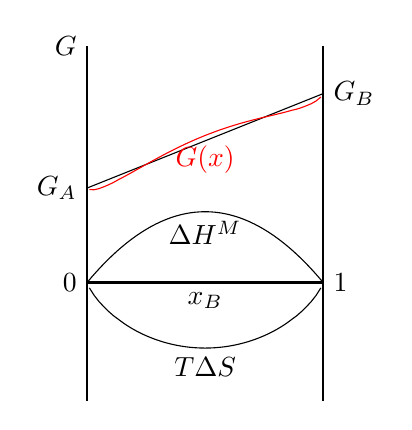
\begin{tikzpicture}[scale=3]
            \draw[thick] (0,0) node[anchor=east]{0} --(0.5,0) node[anchor=north] {$x_B$}--(1,0) node[anchor=west]{1};
            \draw[thick] (0,-0.5) -- (0,0.4) node[anchor=east]{$G_A$}--(0,1) node[anchor=east]{$G$};
            \draw[thick] (1,-0.5) -- (1,0.8) node[anchor=west]{$G_B$}--(1,1);
            %G(0)
            \draw[thin] (0,0.4)--(1,0.8);
            %T\Delta S
            \draw[domain=0.01:0.5] plot(\x,{0.4*(\x*ln(\x)+(1-\x)*ln((1-\x)))})
                node[below] {$T\Delta S$};
            \draw[domain=0.5:0.99] plot(\x,{0.4*(\x*ln(\x)+(1-\x)*ln((1-\x)))});
            %\Delta H
            \draw[domain=0:0.5] plot(\x,{1.2*(\x*(1-\x))})
                node[below] {$\Delta H^M$};
            \draw[domain=0.5:1] plot(\x,{1.2*(\x*(1-\x))});
            
            %G(x)
            \draw[red,domain=0.01:0.5] plot(\x,{0.4*\x+0.4+1.2*(\x*(1-\x))+0.4*(\x*ln(\x)+(1-\x)*ln((1-\x)))})
                node[below] {$G(x)$};
            \draw[red,domain=0.5:0.99] plot(\x,{0.4*\x+0.4+1.2*(\x*(1-\x))+0.4*(\x*ln(\x)+(1-\x)*ln((1-\x)))});        
        \end{tikzpicture}
        %\caption{$\Delta H^M<0$,混合时结合能小于零的自由能曲线。}
        \label{subfig:低温下混合时结合能增加的自由能曲线}
    }
    \subfloat[$T=0$]
    {
        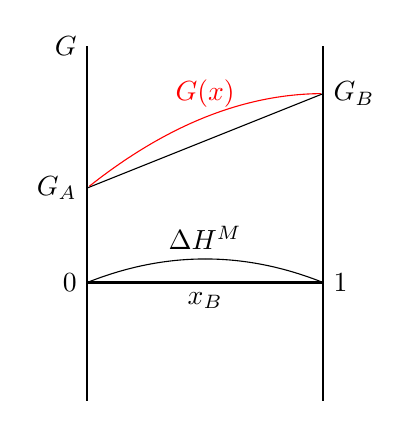
\begin{tikzpicture}[scale=3]
            \draw[thick] (0,0) node[anchor=east]{0} --(0.5,0) node[anchor=north] {$x_B$}--(1,0) node[anchor=west]{1};
            \draw[thick] (0,-0.5) -- (0,0.4) node[anchor=east]{$G_A$}--(0,1) node[anchor=east]{$G$};
            \draw[thick] (1,-0.5) -- (1,0.8) node[anchor=west]{$G_B$}--(1,1);
            %G(0)
            \draw[thin] (0,0.4)--(1,0.8);
            %T\Delta S
            %\draw[domain=0.01:0.5] plot(\x,{0.4*(\x*ln(\x)+(1-\x)*ln((1-\x)))})
            %    node[below] {$T\Delta S$};
            %\draw[domain=0.5:0.99] plot(\x,{0.4*(\x*ln(\x)+(1-\x)*ln((1-\x)))});
            %\Delta H
            \draw[domain=0:0.5] plot(\x,{0.4*(\x*(1-\x))})
                node[anchor=south] {$\Delta H^M$};
            \draw[domain=0.5:1] plot(\x,{0.4*(\x*(1-\x))});
            
            %G(x)
            \draw[red,domain=0.01:0.5] plot(\x,{0.4*\x+0.4+0.4*(\x*(1-\x))})
                node[anchor=south] {$G(x)$};
            \draw[red,domain=0.5:0.99] plot(\x,{0.4*\x+0.4+0.4*(\x*(1-\x))});        
        \end{tikzpicture}
        %\caption{$\Delta H^M<0$,混合时结合能小于零的自由能曲线。}
        \label{subfig:绝对零度下混合时结合能增加的自由能曲线}
    }
    %\end{subfigure}
    \caption{混合时结合能增加的在不同温度下的自由能曲线}

\end{figure}

                
                当$T\geq\frac{\alpha^{\prime}}{2R}$时,混合所提高的内能全部由热温熵来补充,$\Delta G^m\leq0$,曲线仍然为下垂曲线,仅仅是下垂的程度小一点,如\autoref{subfig:高温下混合时结合能增加的自由能曲线}所示。

                在低温情况下,$T<\frac{\alpha^{\prime}}{2R}$时,构成的曲线有三个极值点和两个拐点,在靠近坐标轴($x$接近0或1)处为上凹曲线,有两个极小值,而中部位凹向朝下的上凸曲线,会有一极大值,如\autoref{subfig:低温下混合时结合能增加的自由能曲线}所示。
                在这种情况下,存在两种必然的规律:
                \begin{enumerate}
                    \item[1] 任何一个组元都可以少量溶解其它组元,不可能得到绝对的纯净物质;
                    \item[2] 当出现上凸时,吉布斯自由能会提高,自发的趋势是形成两相混合物可以降低体系的自由能,两组元表现为有限溶解。
                \end{enumerate}
    \section{均匀形核}
        相变动力学\index{相变动力学}是讨论相变的过程和速度的,新相的形核\index{形核}和长大\index{长大}是动力学的两个基本问题。

        即使在宏观的单相均匀系统中,也存在着微观的不均匀性,存在局部的能量、密度、成分组态的涨落。Gibbs将这种涨落分为两类:
        \begin{enumerate}
            \item[1] 在\textbf{很小的体积}内存在着剧烈的原子再分布,在亚稳的母相中形成\textbf{新相胚芽},当这种胚芽超过临界尺寸\index{形核!临界尺寸},就变成稳定的新相核心而自发长大,金属和合金中的转变多数如此;
            \item[2] 在\textbf{大的体积内}原子的少量调整,\textbf{转变在整个体积范围内进行},如有序-无序转变\index{有序-无序转变}。
        \end{enumerate}

        以纯金属的凝固为例,假设在$L$中形成半径为$r$的晶核\index{形核!晶核}$s$,固体和液体的体积为$V_s$和$V_L$,固体和液体单位体积的自由能为$G_v^s$、$G_v^L$,$A_{SL}$为两相之间面积,$r_{SL}$为两相的界面能。

        假设发生相变的过程中没有体积变化,没有形核时,体系的自由能为
        \begin{equation}
            G_1=\left( V_s+V_l \right)G_v^L,
        \end{equation}
        则体系中出现晶核的自由能为:
        \begin{equation}
            G_2=V_sG_v^S+V_LG_v^L+A_{SL}\gamma_{SL},
        \end{equation}
        所以形核时的自由能变化为
        \begin{equation}
            \Delta G_v=G_2-G_1=-V_S\cdot \Delta G_v++A_{SL}\gamma_{SL},
        \end{equation}
        式中$\Delta G_v=G_v^L-G_v^S$。
        
        假设晶核为球形,则固液界面面积和固体体积为
        \begin{equation}
            A_{SL}=4\pi r^2, V=\frac{4}{3}\pi r^3,
        \end{equation}
        形核的自由能变化量为
        \begin{equation}
            \Delta G_r=-\frac{4}{3}\pi r^3\Delta G_v+4\pi r^2\gamma_{SL},
        \end{equation}
        在平衡状态下,对$r$求导,
        \begin{equation}
            \frac{\dif \Delta G_r }{\dif r}=-4\pi r^2\Delta G_v+8\pi r\gamma_{SL},
        \end{equation}
        令导数为零,此时的晶核半径为临界晶核尺寸\index{临界晶核尺寸}
        \begin{equation}
            r^*=\frac{\gamma_{SL}}{\Delta G_v}.
        \end{equation}
        自由能改变量为
        \begin{equation}
            \Delta G^*=\frac{16\pi}{3}\left( \frac{\gamma_{SL}^3}{\Delta G_v^2} \right),
        \end{equation}
        根据自由能的二阶导数可知,此时的自由能为极大值。因此只有半径大于临界晶核尺寸的晶核才能继续长大,而小于该尺寸的晶核则消失。
        临界晶核对于的自由能变化量$\Delta G^*$为形核功,即核长大到$r^*$所需克服的势垒。

        形核功的量值是临界球形晶核表面能的$1/3$,也就是说,球形晶核的表面能的$2/3$由新相的自由能下降给出,
        $1/3$依靠热涨落。这一过程称为\textbf{热激活过程}\index{形核!热激活过程}。

        在凝固过程中,要达到临界半径,需要温度上提供足够的过冷度,假设熔点温度为$T_m$,外界温度与熔点温度差为$\Delta T$,
        此时的自由能变化量为
        \begin{equation}
            \Delta G_v=\frac{\Delta T\cdot\Delta H_m}{T_m},
        \end{equation}
        代入临界半径表达式为
        \begin{equation}
            r^*=\frac{2\gamma_{LS}T_m}{\Delta H_m\cdot\Delta T},
        \end{equation}
        因此当$\Delta T=0$,$\Delta G^*\to0$,不能形核,过冷度越大,越易形核。
    \section{形核速率及均匀形核在固态转变中的推广}
        在液态的情况下,金属中也会存在一些小区域具有固态的密堆结构,本章将对这些小区域进行讨论。

        假设在单位体积内,由$i$个分子组成半径为$r$的胚芽数为$n_i$,而单分子数目为$n$,
        而单位体积中独立质点数$N$为
        \begin{equation}
            N=n+\sum_{i\geq2}n_i,
        \end{equation}
        由于$\sum_{i\geq2}n_i\ll n$,所以$N$约等于单位体积中的分子数。从统计方面考虑,胚芽数$n_i$服从玻尔兹曼分布:
        \begin{equation}
            n_i=N e^{-\frac{\Delta G_r}{kT}},
        \end{equation}
        临界核心数$n_i^*$为
        \begin{equation}
            n_i^*=N e^{-\frac{\Delta G_r^*}{kT}},
        \end{equation}
        其中$\Delta G_r^*$为形核功。

        在临界核心上痛殴分子碰撞再增加一个分子,它就可以克服势垒称为稳定的新相核心。
        定义单位体积中单位时间内形成的新相稳定核心的数目为形核速率\index{形核速率}$I$,
        所以形核速率$I$正比于临近核心的分子加入核心的频率$\omega$,即
        \begin{equation}
            I=\omega\cdot n_i^*=\omega N e^{-\frac{\Delta G_r^*}{kT}}\label{形核速率},
        \end{equation}
        $\omega$取决于原子振动频率、扩散激活能、晶核的表面积等。

        \subsection{形核引起的晶格畸变}
            在金属相变的过程中,由于晶核周围的体积和形状可能发生变
            化,或者晶核受到周围晶格的限制,使得晶核中的原子不能处
            在平衡位置,这两种情况都消耗弹性应变能$\varepsilon$,这种弹性应变
            能通过扩散和范性流变才能松弛。

            假定应变能正比于晶核的体积,则形核的自由能写作
            \begin{equation}
                \Delta G_r=-\frac{4}{3}\pi \cdot r^3(\Delta G_v+\varepsilon)+4\pi\cdot r^2\cdot\gamma_{SL},
            \end{equation}
            临界半径变为
            \begin{equation}
                r^*=\frac{2\gamma_{SL}}{\Delta G_v+\varepsilon},
            \end{equation}
            形核功为
            \begin{equation}
                \Delta G^*=\frac{16\pi \gamma^3_{SL}}{3(\Delta G_v+\varepsilon)^2}.
            \end{equation}
            另外,假设晶核的表面积对此时的邻近核心的分子加入核心的频率$\omega$没有影响,可以写为
            \begin{equation}
                \omega=ve^{-\frac{\Delta G_m}{kT}},
            \end{equation}
            其中$v$是原子振动频率\index{形核速率!原子振动频率},$\Delta G_m$是原子扩散的激活能\index{形核速率!扩散激活能}。所以\autoref{形核速率}可以写为
            \begin{equation}
                I=Nve^{-\frac{\Delta G^*+\Delta G_m}{kT}}\label{考虑外来扩散原子的形核速率},
            \end{equation}
            式中,$Nv$对$I$的影响很小,形核速率强烈依赖指数因子,也就是形核功和原子扩散激活能。
            对于固态相变,合理的数量级为
            \begin{equation*}
                Nve^{-\frac{\Delta G_m}{kT}}\simeq 10^{30},I=10^{30}e^{-\frac{\Delta G^*}{kT}}.
            \end{equation*}

            由于$\Delta G^*$因过冷度$\Delta T$的增大而减小,所以\textbf{形核速率强烈依赖于温度}。
            当$\Delta T\to0$,$\Delta G^*\to\infty$,$I\to0$,$\Delta T$增大,形核速率$I$存在极值,
            先增大后减小。

            \begin{figure}[ht]
                \centering
                    \subfloat[某合金的局部相图。]
                    {
                        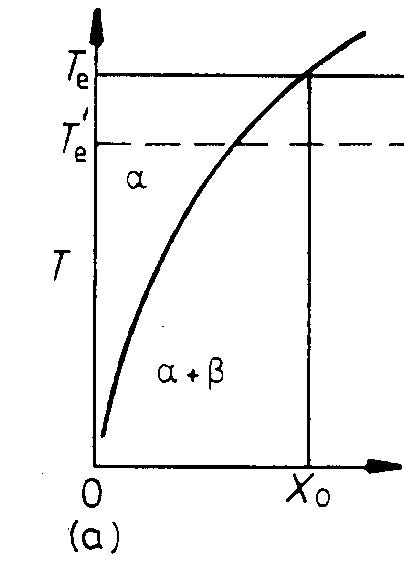
\includegraphics{fig/nucleai_with_temperature/a.jpg}
                        \label{subfigure:某合金的局部相图}
                    }
                    \subfloat[相图的有效推动能量与形核功与转变温度之间的关系。]
                    {
                        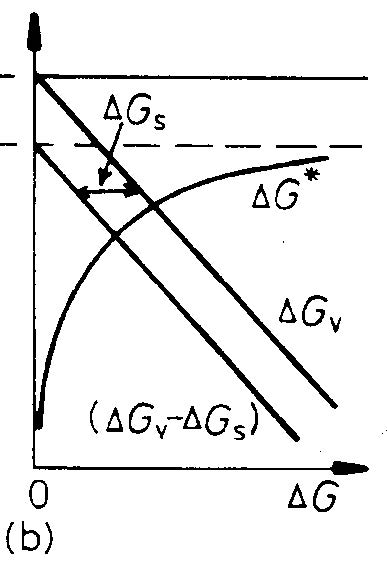
\includegraphics{fig/nucleai_with_temperature/b.jpg}
                    }
                    \\
                    \subfloat[确定$I$的两个指数项与温度的关系。]
                    {
                        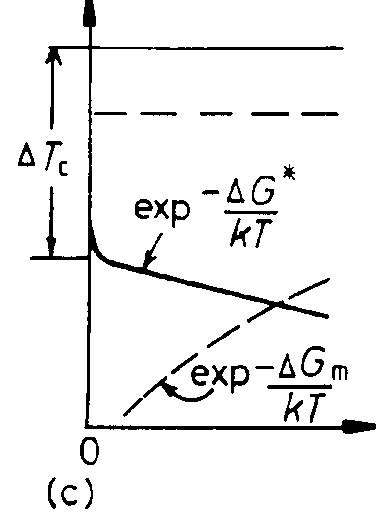
\includegraphics{fig/nucleai_with_temperature/c.jpg}
                    }
                    \subfloat[$I $随温度的变化。]
                    {
                        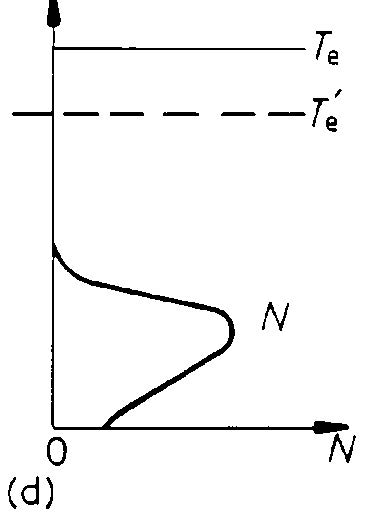
\includegraphics{fig/nucleai_with_temperature/d.jpg}
                        \label{subfigure:$I $随温度的变化}
                    }
                \caption{均匀形核速率$I$与转变温度之间的关系。}
                \label{均匀形核速率I与转变温度之间的关系}
            \end{figure}

            从\autoref{subfigure:某合金的局部相图}可知,成分为$x_0$的合金,其固溶温度为$T_e$,为了抵消应变能$\Delta G_\varepsilon$,
            必须过冷到$T_e^{\prime}$才能析出第二相$\beta$。形核速率随$T$的变化如\autoref{subfigure:$I $随温度的变化}所示,
            在高温下,沉淀的推动能量很小,因为$\Delta G^*$很大,所以$I$很小;在低温情况下,由于扩散很慢,所以$I$也很小,在中间某一个温度,
            $I$有极大值。

        \subsection{相界面性质的影响}

            界面能\index{界面能}$\gamma$的来源可以分为两部分,
            \begin{itemize}
                \item[1] 一部分是在母相中形成新相界面时,同类键和异类键的数量变化引起的,称为界面能中的\textbf{化学项}\index{界面能!化学项};
                \item[2] 另一部分是界面结构引起的 (如界面上产生的位错),称为界面能中的\textbf{结构项}\index{界面能!结构项}。
            \end{itemize}
            
            如果新相和母相的晶体结构和取向相同,电阵常数也非常接近,形成\textbf{完全共格界面}\index{完全共格界面}。界面能
            较小,只包括化学项,结构项(畸变能$\varepsilon$)趋于0,长大速度很快。

            如果完全共格两相的点阵常数不同,就会在界面上引入位错,来减少界面能中的体积应变能,结构项略有增大,形成\textbf{部分共格界面}\index{部分共格界面}。

            若新相通过母相切变形成,某些界面点阵相似,这种界面称为\textbf{切变共格}\index{切变共格}。

            如果所有界面都不共格,称为\textbf{非共格}\index{非共格}新相。

            
        \subsection{非均匀形核(界面形核)}
            形核过程若没有择优地点而称为均匀形核。实际上在金属或合金中,总是存在着界面、位错、夹杂等缺陷,因而
            成为非均匀的择优形核地点。主要是因为在缺陷处存在着畸变,在界面或缺陷处形核,可以消除缺陷,松弛部分能量,从而可以降低形核功。

            以锭模内表面的钢水凝固为例,在界面上形成球冠状的晶核,则有三种界面能$\gamma_{LS}$、$\gamma_{LC}$以及$\gamma_{SC}$,
            分别为液固界面能、液体锭模内壁界面能、固体锭模内壁界面能。达到平衡时,具有接触角,在水平上有
            \begin{equation}
                \gamma_{LC}=\gamma_{SC}+\gamma_{LS}\cos\theta\label{晶核形核过程中的力学平衡},
            \end{equation}
            这里不考虑$\gamma_{LS}$的垂直分量,它与锭模及晶核内聚力平衡,与此处无关系。

            假设晶核的曲率半径为$r$,晶核与锭模的接触面积为$A_1$,则
            \begin{equation}
                A_1=\pi\left( r\sin\theta \right)^2=\pi\cdot r^2\sin^2\theta,
            \end{equation}
            晶核与液体的接触面积为$A_2$,
            \begin{equation}
                A_2=2\pi\cdot r^2(1-\cos\theta),
            \end{equation}
            晶核的体积$V$为
            \begin{equation}
                V=\pi\cdot r^3\frac{2-3\cos\theta+\cos^3\theta}{3},
            \end{equation}
            形核之前,界面能为
            \begin{equation}
                \gamma_{LC}\cdot A_1=\gamma_{LC}\pi r^2\sin^2\theta,
            \end{equation}
            形核后,界面能为
            \begin{equation}
                \gamma_{LS}\cdot A_2+\gamma_{SC}\cdot A_1=\gamma_{LS}2\pi r^2(1-\cos\theta)+\gamma_{SC}\pi r^2\sin^2\theta,
            \end{equation}
            形核前后的界面能变化为
            \begin{equation}
                \begin{aligned}
                    \Delta G_s&=\gamma_{LS}\cdot A_2+\gamma_{SC}- \gamma_{LC}\cdot A_1\\
                    &=2 \pi \cdot r^{2}(1-\cos \theta)+\pi r^{2} \sin ^{2} \theta\left(\gamma_{s c}-\gamma_{L c}\right).
                \end{aligned}
            \end{equation}
            代入\autoref{晶核形核过程中的力学平衡}得到
            \begin{equation}
                \Delta G_{S}=\pi \cdot r^{2} \gamma_{L S}\left(2-3 \cos \theta+\cos ^{3} \theta\right).
            \end{equation}
            晶核形成时化学自由焓变化为
            \begin{equation}
                -V \cdot \Delta G_{v}=-\pi \cdot r^{3} \frac{2-3 \cos \theta+\cos ^{3} \theta}{3} \Delta G_{v},
            \end{equation}
            非均匀形核的自由能总改变量为上两项之和
            \begin{equation}
            \begin{aligned} 
                \Delta G_{\text{非}| \mathrm{E}} &=\Delta G_{s}+\left(-V \cdot \Delta G_{v}\right) \\ 
                &=\left(\pi \cdot r^{2} \cdot \gamma_{L S}-\frac{\pi \cdot r^{3}}{3} \cdot \Delta G_{v}\right) \cdot\left(2-3 \cos \theta+\cos ^{3} \theta\right) \\ 
                &=\left(-\frac{4 \pi \cdot r^{3}}{3} \Delta G_{v}+4 \pi \cdot r^{2} \gamma_{L S}\right). \cdot \frac{2-3 \cos \theta+\cos ^{3} \theta}{4} 
            \end{aligned}
            \end{equation}
            类似于前面求均匀形核功时的推导,平衡时有
            \begin{equation}
                \frac{\dif\left(\Delta G_{ \text{非}}\right)}{\dif r}=\left(-4 \pi \cdot r^{2} \cdot \Delta G_{v}+8 \pi \cdot r \cdot \gamma_{LS}\right) \cdot \frac{2-3 \cos \theta+\cos ^{3} \theta}{4}=0,
            \end{equation}
            此时临界半径为
            \begin{equation}
                r^*=\frac{2\gamma_{LS}}{\Delta G_v},
            \end{equation}
            对应的非均匀形核功为
            \begin{equation}
                \Delta G_{\text{非}}^{*}=\frac{16 \pi \gamma_{L S}^{3}}{3 \Delta G_{v}^{2}} \cdot \frac{2-3 \cos \theta+\cos ^{3} \theta}{4},
            \end{equation}
            对于均匀形核,形核功为
            \begin{equation}
                \Delta G^*_{\text{均}}\cdot\frac{2-3 \cos \theta+\cos ^{3} \theta}{4},
            \end{equation}
            由于
            \begin{equation}
                \frac{2-3 \cos \theta+\cos ^{3} \theta}{4}=\frac{(2+\cos \theta)(1-\cos \theta)^{2}}{4} \leq 1,
            \end{equation}
            所以,有以下结论:
            \begin{itemize}
                \item[1] $\theta=0$,$\cos\theta=1$,$\Delta G^*_{\text{非}}/\Delta G^*_{\text{均}}=0$,此时称为完全浸润;
                \item[2] $\theta=\frac{\pi}{2}$,$\cos\theta=0$,$\Delta G^*_{\text{非}}/\Delta G^*_{\text{均}}=\frac{1}{2}$;
                \item[3] $\theta=\pi$,$\cos\theta=-1$,$\Delta G^*_{\text{非}}/\Delta G^*_{\text{均}}=1$,此时称为完全不浸润;
                \item[4] 一般情况下,非均匀形核的形核功比均匀形核小。
            \end{itemize}
    
    \section{新相的长大}
        在讨论完形核过程,接下来讨论相的长大过程。相长大有两种形式,分别为扩散型和非扩散型。
        其中扩散性又有两种分别为短程扩散和长程扩散,两种的扩散速度不同。
        
        \subsection{界面控制的长大过程}
            对于没有成分变化的转变,比如多形性转变、有序-无序转变等,可以吧新相长大的过程看出纯粹是$\alpha\to\beta$相界的移动过程。

            相变$\alpha\to\beta$的驱动力是自由能的变化$\Delta G_v$,阻力是克服势垒$\Delta G_m$。
            根据统计力学,原子发生$\alpha\to\beta$转变的频率为
            \begin{equation}
                v_{\alpha \beta}=v \exp \left(-\frac{\Delta G_{m}}{k T}\right),
            \end{equation}
            式中,$v$为原子振动频率。而原子反向由$\beta\to\alpha$的频率为
            \begin{equation}
                v_{\beta \alpha}=v \exp \left(-\frac{\Delta G_{m}-\Delta G_{v}}{k T}\right),\Delta G_{v}<0,
            \end{equation}
            则原子由$\alpha\to\beta$的迁移频率$v^\prime$为:
            \begin{equation}
                v^{\prime}=v_{\alpha \beta}-v_{\beta \alpha}=v \exp \left(-\frac{\Delta G_{m}}{k T}\right)\left[1-\exp \left(\frac{\Delta G_{v}}{k T}\right)\right],
            \end{equation}
            假设迁移距离为$\lambda$,则$\beta$长大速度为
            \begin{equation}
                u=\lambda v^{\prime}=\lambda v \exp \left(-\frac{\Delta G_{m}}{k T}\right)\left[1-\exp \left(\frac{\Delta G_{v}}{k T}\right)\right].
            \end{equation}

            根据温度和自由能变化情况不同,可以分为以下几种情况:
            \begin{itemize}
                \item[1] 当$\Delta T$很小,$|\Delta G_v|$也很小,而且$|\Delta G_v|\ll kT$,则有
                        \begin{equation}
                            u=\lambda v\left(-\frac{\Delta G_{v}}{k T}\right) \exp \left(-\frac{\Delta G_{m}}{k T}\right);
                        \end{equation} 
                        跨越相界的扩散系数为$D=\lambda^2v \exp \left( -\frac{\Delta G_m}{kT} \right)$,所以有
                        \begin{equation}
                            u=\frac{D}{\lambda}\left(-\frac{\Delta G_{v}}{k T}\right),
                        \end{equation}
                        也就是当$\Delta T$很小,$u\propto|\Delta G_v|$,并且随温度下降而增加,虽然扩散系数下降,但是并不会产生较大影响;
                \item[2] 如果$\Delta T$很大,使$|\Delta G_v|\gg kT$,则有
                        \begin{equation}
                            u=\lambda v \exp \left(-\frac{\Delta G_{m}}{k T}\right)=\frac{D}{\lambda},
                        \end{equation} 
                        长大速度$u\propto D$,并且随温度下降而减小。
            \end{itemize}
            在某一温度,长大速率有极大值。当形核和长大速率都大时,相变最快,因而使温度-时间-转变曲线呈字母C的形状。在恒温转变过程中,新相恒速长大,其线度$\propto$长大时间。
        \subsection{扩散控制的长大过程}
            对于一些有成分变化(如连续沉淀)的转变,新相的长大依靠溶质原子的长程扩散。

            
    \section{过饱和固溶体的脱溶沉淀}
    \section{调幅分解}
    \section{马氏体相变}
\part{考试内容}
	\chapter{晶体缺陷与强化}
    \section{考试安排}
        考试成绩80\%。
        5个名词、4个简答、2个辨析,说明对错和理由,作图题
        2道大题关于扩散和凝固。

        点缺陷7分、名词解释、线缺陷大约15分、强化8分、断裂10分、单晶滑移8分、回复与再结晶10分。
    \section{问题}
    \begin{itemize}
        \item[1] 从几何形态上说,晶体缺陷分哪几类,试举几个典型例子,位错与空位之间有何相互作用?
        \item[2] 为何为点缺陷的形成能和迁移能,为什么说点缺陷是一种热力学平衡缺陷?一定温度下空位平衡浓度的表达式是什么,有什么特点?
        \item[3] 什么叫非平衡点缺陷?试举例说明它的产生方法?
        \item[4] 什么叫位错,位错密度的表达式是什么?
        \item[5] 试总结与比较刃型,螺型及混合位错下列方面的异同(从结构类型,柏式矢量,应力场特点,应变能和张力方面进行描述)。
        \item[6] 何谓柏格斯矢量,柏氏矢量的特点及确定方法。单位长位错的应变能及张力近似表达式是什么?
        \item[7] 为何要引入位错的点阵模型,它能说明什么问题。什么叫位错线宽度,位错中心能量?定性叙述位错的 Pelels模型。
        \item[8] 计算位错运动引起的变形及位错引起的晶体弯曲?
        \item[9] 什么叫作用在位错上的力,这力的大小,方向及特点是什么(分别讨论滑移力,攀移力,化学力),位错受力的 peach公式及由此计算位错在应力场中受到的滑移和攀移力。 
        \item[10] 分类叙述不同类型平行位错线间相互作用力大小,方向及特点?何为位错塞积?
        \item[11] 不同的两条位错相遇时会发生哪些现象?位错反应发生的基本条件是什么?
        \item[12] 不同面位错相互切割后会在各位错线上造成什么后果?什么叫割阶以及它们的运动方式?
        \item[13] 试述位错FR源的动作原理及动作应力表达式?
        \item[14] 什么叫层错?简述面心立方晶体中的不全位错(半,偏位错),扩展位错?什么叫全位错和不动位错?试比较全位错和不全位错的异同点。
        \item[15] 为何说晶界有5个自由度,什么叫扭转晶界,倾转晶界及亚品界?
        \item[16] 晶界为何具有能量,近代关于晶界结构的基本看法是什么?
    \end{itemize}
    关于固溶体和扩散和相变的问题:
    \begin{enumerate}
        \item[1] 固溶度的影响因素,各因素的机理?
        \begin{enumerate}
            \item 电子浓度,Hume-Rothery定律
            \item 尺寸、
            \item 化学亲合力、
        \end{enumerate} 
        \item[2] 系统形成有序固溶体的条件是什么
        \begin{enumerate}
            \item 动力:内能降低,倾向于异种原子成键;
            \item 阻力:组态熵
        \end{enumerate} 
        \item[3] 中间相的类型
        \begin{enumerate}
            \item 电子化合物
            \item 正常家化合物
            \item 尺寸因素化合物
            \item 脆性相
        \end{enumerate} 
        \item[4] 元素的负电性是什么含义,如何作用形成化合物?
        \item[5] 原子成功跃迁的条件,影响因素是什么?
        \begin{enumerate}
            \item 与熔点有关,熔点越高,原子越稳定,不易跃迁。
        \end{enumerate} 
        \item[6] 扩散过程的两个基本方程,简述内容
        \begin{enumerate}
            \item 菲克第一定律:解释各个物理量含义和单位;
            \item 菲克第二定律
        \end{enumerate} 
        \item[7] 写出扩散过程的决定因素?
        \begin{enumerate}
            \item 化学位梯度
        \end{enumerate} 
        \item[8] 扩散热激活能和影响因素?
        \begin{enumerate}
            \item 扩散系数与温度的关系为$D=D_0\exp\left( -\frac{Q}{RT} \right)$,其中$Q$为扩散激活能;
            \item 扩散激活能与成分、结构、与温度无关。
        \end{enumerate} 
        \item[9] 扩散系数的影响因素?
        \begin{enumerate}
            \item $D=\frac{1}{6}\alpha^2\Gamma=\frac{1}{6}\alpha^2Zp_v\omega$,
            \item 温度
            \item 成分
            \item 结构
        \end{enumerate} 
        \item[10] 卡根达二效应、达肯方程、原始焊接平面、matano面和标记面分意义
        \item[11] 在\ce{Fe-C}相图中,温度高于\SI{923}{\celsius}和在\SIrange{727}{912}{\celsius}之间两种情况下渗碳,碳浓度曲线有何不同?画出来,如何证明两相区($\alpha+\gamma$)不存在?
        \item[12] 给出钍在钨中的体扩散系数、晶粒间扩散系数和表面扩散系数的大小顺序,说明该顺序与温度的关系?
        \item[13] 为什么会出现上坡扩散?是否与菲克定律矛盾?
        \item[14] 影响扩散的因素有那些
        \item[15] 简述间隙固溶体和间隙相?
        \item[16] 形成有序固溶体的阻力是什么?有序-无序转变是不是相变?
        \item[17] 界面能的来源有哪些?
        \item[18] 简述形核的类型和特点,影响形核的因素有什么?
        \item[19] 什么叫脱溶惯序?为什么会发生?
        \item[20] 什么叫正脱溶、负脱溶?举例说明
        \item[21] 从比热-温度曲线说明预沉淀过程。
        \item[22] 什么是GP区?简述特点
        \item[23] 为什么GP区有片状球状,影响因素是什么?
        \item[24] 新相长大的途径有什么?影响因素是什么?
        \item[25] 沉淀相为什么会粗化?其粗化过程是什么?
        \item[26] 发生调幅分解的条件是什么?
        \item[27] 马氏体形貌的控制因素是什么?
        \item[28] 简述马氏体相变,是不是一级相变,为什么?
        \item[29] 马氏体相变类型有哪些?
        \item[30] 共析转变过程,其特点是什么?
    \end{enumerate}
\clearpage

\backmatter


%\cleardoublepage
\phantomsection
\addcontentsline{toc}{chapter}{索引}
\printindex

\cleardoublepage
\phantomsection
\addcontentsline{toc}{chapter}{参考文献}
\bibliographystyle{unsrt}
\bibliography{reference.bib}


\end{document}
